%%%%% Set up %%%%%

% Set document style and font size
\documentclass[12pt]{article}\usepackage[]{graphicx}\usepackage[]{color}
%% maxwidth is the original width if it is less than linewidth
%% otherwise use linewidth (to make sure the graphics do not exceed the margin)
\makeatletter
\def\maxwidth{ %
  \ifdim\Gin@nat@width>\linewidth
    \linewidth
  \else
    \Gin@nat@width
  \fi
}
\makeatother

\definecolor{fgcolor}{rgb}{0.345, 0.345, 0.345}
\newcommand{\hlnum}[1]{\textcolor[rgb]{0.686,0.059,0.569}{#1}}%
\newcommand{\hlstr}[1]{\textcolor[rgb]{0.192,0.494,0.8}{#1}}%
\newcommand{\hlcom}[1]{\textcolor[rgb]{0.678,0.584,0.686}{\textit{#1}}}%
\newcommand{\hlopt}[1]{\textcolor[rgb]{0,0,0}{#1}}%
\newcommand{\hlstd}[1]{\textcolor[rgb]{0.345,0.345,0.345}{#1}}%
\newcommand{\hlkwa}[1]{\textcolor[rgb]{0.161,0.373,0.58}{\textbf{#1}}}%
\newcommand{\hlkwb}[1]{\textcolor[rgb]{0.69,0.353,0.396}{#1}}%
\newcommand{\hlkwc}[1]{\textcolor[rgb]{0.333,0.667,0.333}{#1}}%
\newcommand{\hlkwd}[1]{\textcolor[rgb]{0.737,0.353,0.396}{\textbf{#1}}}%
\let\hlipl\hlkwb

\usepackage{framed}
\makeatletter
\newenvironment{kframe}{%
 \def\at@end@of@kframe{}%
 \ifinner\ifhmode%
  \def\at@end@of@kframe{\end{minipage}}%
  \begin{minipage}{\columnwidth}%
 \fi\fi%
 \def\FrameCommand##1{\hskip\@totalleftmargin \hskip-\fboxsep
 \colorbox{shadecolor}{##1}\hskip-\fboxsep
     % There is no \\@totalrightmargin, so:
     \hskip-\linewidth \hskip-\@totalleftmargin \hskip\columnwidth}%
 \MakeFramed {\advance\hsize-\width
   \@totalleftmargin\z@ \linewidth\hsize
   \@setminipage}}%
 {\par\unskip\endMakeFramed%
 \at@end@of@kframe}
\makeatother

\definecolor{shadecolor}{rgb}{.97, .97, .97}
\definecolor{messagecolor}{rgb}{0, 0, 0}
\definecolor{warningcolor}{rgb}{1, 0, 1}
\definecolor{errorcolor}{rgb}{1, 0, 0}
\newenvironment{knitrout}{}{} % an empty environment to be redefined in TeX

\usepackage{alltt}

% File path to resources (style file etc)
\newcommand{\locRepo}{csas-style}

% Style file for DFO Technical Reports
\usepackage{\locRepo/tech-report}

% header-includes from R markdown entry
\usepackage{float}
\usepackage{underscore}
\usepackage{pdfpages}
\usepackage{pdflscape}
\usepackage{booktabs}
\usepackage{helvet}
\renewcommand{\familydefault}{\sfdefault}
\usepackage{colortbl}
\usepackage{xcolor}
\definecolor{ltgray}{HTML}{DEDEDE}
\usepackage{caption}
\usepackage{array}
\captionsetup{justification=justified, singlelinecheck=off, font=small}
\usepackage[labelfont=bf]{caption}
\usepackage{tabu}
\usepackage[utf8]{inputenc}
\DeclareUnicodeCharacter{2212}{-}

%%%%% Variables %%%%%

% New definitions: Title, year, report number, authors
% Protect lower case words (i.e., species names) in \Addlcwords{}, in "TechReport.sty"
\newcommand{\trTitle}{Mission Report for the Maritimes Region Atlantic Zone Monitoring Program 2025 Spring Survey (EN728)}
\newcommand{\trYear}{2025}
\newcommand{\trReportNum}{xxxx}
\newcommand{\trDOI}{\#\#.\#\#\#\#/xxxxx}
% Optional
\newcommand{\trAuthFootA}{Email: \link{mailto:Lindsay.Beazley@dfo-mpo.gc.ca}{\nolinkurl{Lindsay.Beazley@dfo-mpo.gc.ca}} \textbar{} telephone: (902) 225-3743}
\newcommand{\trAuthsLong}{Lindsay Beazley\textsuperscript{1}, Diana Cardoso\textsuperscript{1}, Christopher Gordon\textsuperscript{1}, and Carina Gjerdrum\textsuperscript{2}}
\newcommand{\trAuthsBack}{Beazley, L., Cardoso, D., Gordon, C., and Gjerdrum, C.}

% New definition: Address
\newcommand{\trAddy}{\textsuperscript{1}Ocean and Ecosystem Sciences Division\\
Fisheries and Oceans Canada\\
Bedford Institute of Oceanography\\
P.O. Box 1006\\
Dartmouth, Nova Scotia\\
Canada, B2Y 4A2\\
\textsuperscript{2}Canadian Wildlife Service\\
Environment and Climate Change Canada\\
45 Alderney Drive\\
Dartmouth, Nova Scotia\\
Canada, B2Y 2N6\\}

% Abstract
\newcommand{\trAbstract}{Fisheries and Oceans Canada's (DFO) Maritimes Region Atlantic Zone Monitoring Program 2025 spring survey was conducted on the Research Vessel \emph{Endeavor} from March 29 to April 18, 2025. A total of 13 scientific staff participated in the mission and led the deployment of various oceanographic equipment across a network of fixed monitoring stations, including CTD-Rosette deployments for the collection of vertical profiles of e.g., temperature and salinity, and water samples from pre-determined depths, vertical ring net tows for zooplankton sample collection, and Argo float deployments in support of the International Argo program. Additionally, a single passive acoustic monitoring mooring was deployed in Roseway Basin, Scotian Shelf, and a series of acoustic receiver moorings were recovered in the Gully Marine Protected Area (MPA) in support of a DFO-Ocean Tracking Network collaboration to study the movement of tagged species in and around the MPA. In collaboration with the Woods Hole Oceanographic Institution, an Imaging Flow Cytobot was used to collect high-resolution images of phytoplankton from surface waters sampled while underway. This report provides an overview of the mission's objectives, achievements, impacts, gear operations and operational issues. A summary of the seabird and marine mammal observations collected during the mission is presented, as is the vertical structure in temperature, salinity, and dissolved oxygen for each station occupied.}

% Resume (i.e., French abstract)
\newcommand{\trResume}{To be translated}

\newcommand{\trISBN}{}

\DeclareGraphicsExtensions{.png,.pdf}
%%%%% Start %%%%%

% Start the document
\IfFileExists{upquote.sty}{\usepackage{upquote}}{}

% commands and environments needed by pandoc snippets
% extracted from the output of `pandoc -s`
%% Make R markdown code chunks work
\usepackage{array}
\usepackage{amssymb,amsmath}
\usepackage{color}
\usepackage{fancyvrb}

% From default template:
\newcommand{\VerbBar}{|}
\newcommand{\VERB}{\Verb[commandchars=\\\{\}]}
\DefineVerbatimEnvironment{Highlighting}{Verbatim}{commandchars=\\\{\},formatcom=\color[rgb]{0.00,0.00,0.00}}
\usepackage{framed}
\definecolor{shadecolor}{RGB}{248,248,248}
\newenvironment{Shaded}{\begin{snugshade}}{\end{snugshade}}
\newcommand{\AlertTok}[1]{\textcolor[rgb]{0.94,0.16,0.16}{#1}}
\newcommand{\AnnotationTok}[1]{\textcolor[rgb]{0.56,0.35,0.01}{\textbf{\textit{#1}}}}
\newcommand{\AttributeTok}[1]{\textcolor[rgb]{0.77,0.63,0.00}{#1}}
\newcommand{\BaseNTok}[1]{\textcolor[rgb]{0.00,0.00,0.81}{#1}}
\newcommand{\BuiltInTok}[1]{#1}
\newcommand{\CharTok}[1]{\textcolor[rgb]{0.31,0.60,0.02}{#1}}
\newcommand{\CommentTok}[1]{\textcolor[rgb]{0.56,0.35,0.01}{\textbf{#1}}}
\newcommand{\CommentVarTok}[1]{\textcolor[rgb]{0.56,0.35,0.01}{\textbf{\textit{#1}}}}
\newcommand{\ConstantTok}[1]{\textcolor[rgb]{0.00,0.00,0.00}{#1}}
\newcommand{\ControlFlowTok}[1]{\textcolor[rgb]{0.13,0.29,0.53}{\textit{#1}}}
\newcommand{\DataTypeTok}[1]{\textcolor[rgb]{0.13,0.29,0.53}{#1}}
\newcommand{\DecValTok}[1]{\textcolor[rgb]{0.00,0.00,0.81}{#1}}
\newcommand{\DocumentationTok}[1]{\textcolor[rgb]{0.56,0.35,0.01}{\textbf{\textit{#1}}}}
\newcommand{\ErrorTok}[1]{\textcolor[rgb]{0.64,0.00,0.00}{\textit{#1}}}
\newcommand{\ExtensionTok}[1]{#1}
\newcommand{\FloatTok}[1]{\textcolor[rgb]{0.00,0.00,0.81}{#1}}
\newcommand{\FunctionTok}[1]{\textcolor[rgb]{0.00,0.00,0.00}{#1}}
\newcommand{\ImportTok}[1]{#1}
\newcommand{\InformationTok}[1]{\textcolor[rgb]{0.56,0.35,0.01}{\textbf{\textit{#1}}}}
\newcommand{\KeywordTok}[1]{\textcolor[rgb]{0.13,0.29,0.53}{\textit{#1}}}
\newcommand{\NormalTok}[1]{#1}
\newcommand{\OperatorTok}[1]{\textcolor[rgb]{0.81,0.36,0.00}{\textit{#1}}}
\newcommand{\OtherTok}[1]{\textcolor[rgb]{0.56,0.35,0.01}{#1}}
\newcommand{\PreprocessorTok}[1]{\textcolor[rgb]{0.56,0.35,0.01}{\textbf{#1}}}
\newcommand{\RegionMarkerTok}[1]{#1}
\newcommand{\SpecialCharTok}[1]{\textcolor[rgb]{0.00,0.00,0.00}{#1}}
\newcommand{\SpecialStringTok}[1]{\textcolor[rgb]{0.31,0.60,0.02}{#1}}
\newcommand{\StringTok}[1]{\textcolor[rgb]{0.31,0.60,0.02}{#1}}
\newcommand{\VariableTok}[1]{\textcolor[rgb]{0.00,0.00,0.00}{#1}}
\newcommand{\VerbatimStringTok}[1]{\textcolor[rgb]{0.31,0.60,0.02}{#1}}
\newcommand{\WarningTok}[1]{\textcolor[rgb]{0.56,0.35,0.01}{\textbf{\textit{#1}}}}
\begin{document}

%%%% Front matter %%%%%

% Add the first few pages
\frontmatter

%%%%% Drafts %%%%%

%\linenumbers  % Line numbers
%\onehalfspacing  % Extra space between lines
\renewcommand{\headrulewidth}{0.5pt}  % Header line
\renewcommand{\footrulewidth}{0.5pt}  % footer line
%\pagestyle{fancy}\fancyhead[c]{Draft: Do not cite or circulate}  % Header text

\newcommand{\lt}{\ensuremath <}
\newcommand{\gt}{\ensuremath >}

%Defines cslreferences environment
%Required by pandoc 2.8
%Copied from https://github.com/rstudio/rmarkdown/issues/1649
% % \newlength{\cslhangindent}
% \setlength{\cslhangindent}{1.5em}
% \newenvironment{cslreferences}%
%   {}%
%   {\par}
% 
%%%%% Main document %%%%%
\section{Mission Overview}\label{mission-overview}

\subsection{Background}\label{background}

As part of a collaborative agreement between Fisheries and Oceans Canada (DFO), Natural Resources of Canada (NRCan), and the University of Rhode Island, U.S.A, the Research Vessel (RV) \emph{Endeavor} was used to deliver DFO's Maritimes Region Atlantic Zone Monitoring Program's (AZMP) 2025 spring survey of the Scotian Shelf and Gulf of Maine. The AZMP was initiated in 1998 with the aim to detect, track, and predict changes in the state and productivity of waters across the northwest Atlantic. The AZMP's sampling strategy in the Maritimes Region is based on high-frequency (weekly, biweekly, monthly) data collection, hydrographic data collection on the winter and summer Ecosystem Trawl Surveys, and dedicated oceanographic surveys conducted each spring and fall. During the EN728 mission, data and sample collection was conducted across a network of fixed monitoring stations spanning from the Gulf of Maine and the Northeast Channel in the west, and across the Scotian Shelf to the Cabot Strait in the east, and included CTD-Rosette deployments for the collection of vertical profile data and water samples for nutrient, salinity, dissolved oxygen, and chlorophyll \emph{a} determination, ocean acidification and phytoplankton monitoring, and vertical ring net tows for the collection of data on zooplankton abundance and biomass.

The RV \emph{Endeavor} is owned by the U.S. National Science Foundation (NSF) and operated under a Charter Party Agreement by the University of Rhode Island (URI) Graduate School of Oceanography to support multidisciplinary oceanographic missions led by both US scientists and the international community. Built in 1975, this 55-metre long vessel contains three lab spaces for science use, a science network for data sharing and access, two overboarding frames on its main deck, the starboard-side J-frame with two winches spooled with 0.322'' electromechanical cable to support CTD-Rosette deployments, and a stern A-frame. The vessel's home port is 215 South Ferry Road, GSO, University of Rhode Island, Narragansett, RI, and missions are scheduled by the University-National Oceanographic Laboratory System (UNOLS) Ship Scheduling Committee. The RV \emph{Endeavor} was previously chartered by DFO in 2017 to deliver the program's fall mission in the Maritimes Region (mission ID EN606).

In addition to the EN728 mission's primary objectives in support of the Maritimes Region AZMP, data and samples were also collected in support of other research and monitoring programs and initiatives led by both DFO and its external partners, including university projects aimed at evaluating aspects of the marine environment (e.g., microbial component) not monitored by DFO (see the \hyperref[mission-achievements]{Mission Achievements} section below for more details).

This report provides an overview of the mission objectives, achievements and impacts, and a summary of operations and data collected.

\subsection{Mission Synopsis}\label{mission-synopsis}

The RV \emph{Endeavor} departed Narragansett, RI on the morning of Monday March 24, 2025 and began its transit to Nova Scotia for the start of the EN728 mission. The transit took over 48 hours, with the vessel meeting the Halifax harbour pilot at 13:30 ADT on Wednesday March 26. Upon arrival, the \emph{Endeavor} berthed along the south side of the Bedford Institute of Oceanography's finger pier, where it remained for mobilization. On Thursday March 27, mobilization of science equipment for the EN728 mission began at 08:00 ADT. A series of steel cages with equipment were brought over to the vessel and loaded onto its main deck using the vessel's knuckleboom crane. The remainder of the day was spent dispersing and setting up various laboratory equipment to the Main, Special Purpose, and Wet laboratories on board.

On Friday March 28, a familiarization meeting was held at 10:30 ADT with URI marine technicians Claire Mayorga and Lynne Butler to review the safety procedures and expectations for scientific operations. Afterwards, the remaining scientific and mooring equipment was loaded on the vessel, and mobilization was completed that afternoon.

After mobilization was completed, chief scientist Lindsay Beazley reviewed the upcoming weather forecasted for the first few days of the mission. A storm was forecasted to impact the Scotian Shelf starting on Monday, March 31, which would cause high winds and seas that would last until Wednesday April 2. In light of this, a decision was made to alter the mission itinerary to facilitate the deployment of a large passive acoustic monitoring (PAM) mooring in Roseway Basin before arrival of the storm. Instead of heading towards Yarmouth Line, the itinerary was revised so that the AZMP's core Browns Bank Line would be occupied first, with deployment of the PAM mooring occurring in between stations BBL\_02 and BBL\_03. This would ensure the PAM mooring was deployed during safety operating conditions.

On Saturday, March 29, all science staff boarded the vessel for 08:00. A ship's familiarization meeting was held with the second officer to review safe operating procedures and drill protocols. At the same time, the RV \emph{Endeavor} prepared for departure, and left the BIO pier at 09:30 ADT after boarding the Halifax Port authority pilot. After transiting through the Halifax Harbour and disembarking the pilot, the vessel headed towards the first station of the mission, the AZMP's high-frequency station Halifax-2 located 30 nm outside the Halifax Harbour. Operations at this station began with a CTD-Rosette deployment, followed by two vertical ring net tows and a secchi disc deployment. After completion of these activities, a decision was made to change the order of operations for all stations going forward so that the vertical ring net tow was completed first and the CTD-Rosette deployment second. This allowed for sampling of the rosette to occur during the transit between stations, and provided unimpeded deck space to safely recover the net and deployment weight.

Upon completion of activities at HL\_02, the RV \emph{Endeavor} proceeded towards the AZMP's Browns Bank Line, where AZMP stations BBL\_01 and BBL\_02 were sampled prior to arrival at the PAM mooring station in Roseway Basin (station ROPB) at \textasciitilde{} 11:45 UTC, Sunday March 30. Deployment of the mooring was finished by 13:00 UTC, and the vessel continued towards the remaining stations on the Browns Bank Line. After completion of the final station on this line, BBL\_07, Monday March 31, the \emph{Endeavor} headed north towards the start of the Yarmouth Line, which was expected to be more sheltered from the pending storm. Upon arrival at YL\_01, conditions were deemed operable, and deployment of the ring net occurred at \textasciitilde{} 19:00 UTC that same day. Conditions remained favourable to continue and complete operations along the Yarmouth Line. Following this, the Portsmouth Line was occupied, followed by the 10 stations of the Northeast Channel Line. The sea state remained high while in this area, resulting in challenging working conditions while sampling on deck and deploying ring nets. On several stations, the ring net crossbow slid down the wire, resulting in aborted operations and a re-deployment of equipment.

Upon completion of the Northeast Channel Line, the vessel proceeded towards the first station on the Halifax Line, HL\_01, arriving at \textasciitilde22:30 UTC on April 4. Over the course of nearly two days, all stations on the Halifax Line were successfully completed, with the first Argo float deployment of the mission occurring on station HL\_07 after completion of ring net and CTD-Rosette operations on Sunday April 6 at \textasciitilde12:00 UTC. Upon completion of the Halifax Line, the vessel proceeded to the next work location, The Gully Marine Protected Area (MPA), where an array of 15 Ocean Tracking Network (OTN) acoustic receiver moorings were planned for recovery. Deployed for approximately 4 years, these moorings were part of a DFO-OTN project to evaluate the movement of tagged species, particularly juvenile Atlantic halibut, in and around the MPA. During the transit to The Gully, the Captain and chief scientist reviewed the upcoming weather conditions for the week, and noted the development of a significant storm that would impact the Sable Island Bank area on the evening of Tuesday April 8 into Wednesday April 9. Consequently, the chief scientist planned to sample as many AZMP CTD-Rosette/ring net stations as possible during the overnight hours of Sunday April 6 to Monday April 7, and position the vessel on the first mooring station, GUL01, at daylight on Monday, April 7.

The vessel arrived AZMP station GUL\_04 at \textasciitilde03:30 UTC on Monday April 7. As sampling from the rosette took longer than anticipated, a decision was made not to sample a second AZMP CTD station, and head to the first mooring station. The vessel arrived at mooring station GUL01 at \textasciitilde{} 11:30 UTC on Monday April 7. Communications were quickly established with the mooring and it was released. The mooring assembly was recovered using the vessel's knuckleboom crane, and the vessel proceeded to the next mooring station, GUL02. After communications were established with the mooring at GUL02 and the command sent to release it, the mooring failed to surface. The health status of the mooring release was evaluated, which indicated a release tilt ranging between 56 and 68\(^\circ\), suggesting the release was not vertical in the water column. Consequently, the mooring at this station could not be recovered. The mooring at GUL03 also did not surface after release, and its tilt status was also higher than expected (68-79\(^\circ\)). The vessel moved on to the remaining moorings (stations GUL04 through GUL15). Communications could not be established with the releases at GUL05 and GUL12. Upon recovering the mooring at the last station of the array (GUL15), the vessel returned to the AZMP stations situated over the thalweg of the Gully, and completed these overnight on April 7 - 8 while continuing to monitor weather conditions. On April 8, a second attempt was made to recover the moorings at stations GUL02, GUL03, GUL05, and GUL12. Communications could be established with GUL12 and it was successfully recovered, but the moorings at GUL02, GUL03, and GUL12 were not recovered.

Upon departure from The Gully MPA, the weather conditions for the eastern Scotian Shelf and Laurentian Channel were reviewed by the chief scientist and Captain. A significant weather system was expected to impact the area, bringing with it significant winds (up to 35 knots) and seas (up to 4.5 m). A decision was made to transit towards the next work area, the Laurentian Channel Mouth (LCM) section, but with the expectation that conditions might not be favourable to conduct science operations. After the vessel arrived at station LCM\_01 at midnight on April 9, the conditions were assessed and deemed unfavourable for science operations. The bridge positioned the vessel to provide the most comfort for those on board, and waited out the storm. Conditions improved enough to allow science operations to continue at 19:00 UTC on April 9. Overall, the storm resulted in a loss of 16 hours to the program. All 10 stations on the LCM line were completed successfully by 19:18 UTC on April 10, and the vessel moved on to its next section, the Louisbourg Line, arriving at LL\_09 at 07:09 UTC on April 11. The second Argo float was deployed after ring net and CTD operations were completed at this station, and the vessel transited north, completing all remaining stations on the Louisbourg Line. Operations at the final station on the line were completed at 16:08 UTC on April 12, and the vessel proceeded to its next work area, the Cabot Strait.

Operations on the Cabot Strait Line (CSL) began at station CSL\_01 located east of Cape Breton, at 00:21 UTC on April 13. Conditions while working in the area were favourable, and no ice was observed. The vessel worked from west to east, completing operations at station CSL\_06 located off Port Aux Basque, Newfoundland, approximately 14 hours later at 14:12 UTC. The vessel then headed towards the last planned section, the St.~Anns Bank (STAB) Line, and started at station STAB\_06. Upon review of the final planned activities for the EN728 mission, it was evident that the planned program would be completed well in advance of the scheduled disembarkation on Saturday April 19. At this point, proposals for additional data collection were reviewed. A set of 7 stations located on the western side of Sable Island that were sampled in 2022 during the spring AZMP mission (AT4802) to evaluate the effects of potential seal fertilization on the water column were added to the program, as were 5 stations on the extended Halifax Line (HL\_08 through HL\_12). Operations at the final station on the St.~Anns Bank Line were completed at 11:26 on Monday April 14, and the vessel proceeded towards Sable Island Bank.

Operations at Sable Island Bank (SIB) station SIB\_11 commenced at 22:37 UTC on Monday April 14. A review of sea surface chlorophyll \emph{a} from satellite imagery (E. Devred, personal communication) indicated high levels of chlorophyll in the area, suggesting the spring bloom was still occurring in the region. The resulting images from the Woods Hole Imaging Flow Cytobot (IFCB) suggested that the bloom was dominated by one species, a member of the genus \emph{Leptocylindrus}, a long, cylindrical diatom. Operations on the 7th SIB station (SIB\_02) were completed on Tuesday April 15 at 21:06, and the vessel proceeded towards the extended Halifax Line.

The chief scientist reviewed the upcoming weather conditions for the central Scotian Shelf with the Captain, and noted that a significant storm would potentially impact the central Scotian Shelf at the location of the extended Halifax Line. Consequently, a decision was made to start at station HL\_08 and work south, completing as many stations on the extended Halifax Line as possible before conditions worsened. The vessel arrived at HL\_08 at 02:33 UTC on April 16 and operations began with deployment of the 202 \(\mu\)m ring net, followed by a CTD-Rosette cast. Conditions began to worsen as the vessel transited south, and when at HL\_11, a decision was made to cancel operations at the final station, HL\_12 and transit back to port. Upon completion of the CTD-Rosette deployment at HL\_11, the vessel departed the extended Halifax Line and transited north towards station HL\_02, arriving at 23:45 UTC on Thursday April 17. Operations began with the deployment of the 202 and 76 \(\mu\)m ring net systems, followed by the CTD-Rosette. Once operations were completed, the vessel transited north towards the Halifax pilot station outside the mouth of Halifax Harbour.

The pilot was scheduled for Friday April 18 at 08:30 AST, one day prior to the mission's scheduled disembarkation. After the pilot boarded, the vessel began its transit through the Halifax Harbour, and arrived at the BIO at \textasciitilde{} 10:00 local time. The vessel berthed along the south side of the BIO finger pier. Demobilization activities began at 12:30 AST. Wire baskets were craned onto the vessel using its knuckleboom crane and filled with science equipment, and transfered back onto the pier where they were forklifted into a storage bay at the BIO. Demobilization activities were completed at \textasciitilde{} 15:00 AST on Friday April 18, marking conclusion of the EN728 mission.

\clearpage

\section{Participants}\label{sec:participants}

A total of 13 scientific staff participated in the EN728 mission (see Table~\ref{tab:table1}), including 9 DFO personnel, 1 seabird observer from Environment and Climate Change Canada's Canadian Wildlife Service, 2 Dalhousie University students representing the laboratories of Drs. Carolyn Buchwald, Julie LaRoche, and Erin Bertrand, and 1 graduate student from the University of Rhode Island's Graduate School of Oceanography. The chief scientist was Lindsay Beazley (OESD-OMOS), with Chris Gordon (OESD-OMOS) as night shift captain. Science staff were split into day (0700-1900) and night (1900-0700) watches.

Mooring technician Adam Hartling from the Ocean Engineering and Technology Section (OETS) led all mooring operations and also assisted with CTD operations and the management of the Deep SUNA data during day shift.

A total of 14 ship's crew sailed on the mission plus 2 URI marine technicians. The lead marine technician was Claire Mayorga (24:00 - 12:00), with Lynne Butler covering 12:00 - 24:00. Both marine technicians assisted with the deployment and recovery of all scientific equipment and led the communications with the winch operator while on deck, and also managed the IFCB system during the mission. The Captain of the vessel was Master Christopher Armanetti.

\hspace*{-0.5in}
\begin{longtable}[t]{>{\raggedright\arraybackslash}p{1em}>{\raggedright\arraybackslash}p{8em}>{\raggedright\arraybackslash}p{10em}>{\raggedright\arraybackslash}p{15em}>{\raggedright\arraybackslash}p{3em}}
\caption{\label{tab:table1}List of science staff that participated in the 2025 spring AZMP mission (EN728). Affiliation is Department-Division-Section. OMOS = Ocean Monitoring and Observation Section; OETS = Ocean Engineering and Technology Section; OSM = Ocean Stressors and Modeling.}\\
\toprule
\begingroup\fontsize{12}{14}\selectfont \textbf{}\endgroup & \begingroup\fontsize{12}{14}\selectfont \textbf{Name}\endgroup & \begingroup\fontsize{12}{14}\selectfont \textbf{Affiliation}\endgroup & \begingroup\fontsize{12}{14}\selectfont \textbf{Duty}\endgroup & \begingroup\fontsize{12}{14}\selectfont \textbf{Shift}\endgroup\\
\midrule
\endfirsthead
\caption[]{\textit{(continued)}}\\
\toprule
\begingroup\fontsize{12}{14}\selectfont \textbf{}\endgroup & \begingroup\fontsize{12}{14}\selectfont \textbf{Name}\endgroup & \begingroup\fontsize{12}{14}\selectfont \textbf{Affiliation}\endgroup & \begingroup\fontsize{12}{14}\selectfont \textbf{Duty}\endgroup & \begingroup\fontsize{12}{14}\selectfont \textbf{Shift}\endgroup\\
\midrule
\endhead

\endfoot
\bottomrule
\endlastfoot
1 & Nicole Smith & DFO-OSASS & Water sampling, filtration & Day\\
2 & Kristen Wilson & DFO-OMOS & Water sampling, filtration & Night\\
3 & Melanie Hardy & DFO-OMOS & CTD acquisition computer & Day\\
4 & Chris Gordon & DFO-OMOS & CTD acquisition computer/Night shift captain & Night\\
5 & Lindsay Beazley & DFO-OMOS & Chief scientist, ring net operator & Day\\
6 & Rebecca Milne & DFO-OMOS & Ring net operator & Night\\
7 & Diana Cardoso & DFO-OESD & Data manager & Night\\
8 & Adam Hartling & DFO-OETS & CTD operations, SUNA sensor & Night\\
9 & Chris Beck & DFO-OETS & CTD operations, SUNA sensor & Day\\
10 & Jacob Comeau-Ouellette & Environment and Climate Change Canada & Seabird Observer & Day\\
11 & Anna Gleason & Dalhousie University & Water sampling, filtration & Day\\
12 & Sofia Dragoti & Dalhousie University & Water sampling, filtration & Night\\
13 & Jasper Meagher & University of Rhode Island & Water sampling, lab support & Day\\*
\end{longtable}
\clearpage

\section{Mission Achievements}\label{mission-achievements}

A total of 14 objectives were identified during the planning stages of the 2025 spring AZMP mission (see Table~\ref{tab:table2}). In addition to the primary objective to collect spring observations of physical, chemical, and lower trophic-level biological parameters across the Scotian Shelf and eastern Gulf of Maine in support of the AZMP, a request was made by DFO's North Atlantic Right Whale Research Unit led by Research Scientist Angelia Vanderlaan, to re-deploy a passive acoustic monitoring (PAM) mooring in Roseway Basin. This mooring was deployed in the fall of 2024 during the DY18402 AZMP mission to monitor the presence and distribution of North Atlantic right whales, but unintentionally resurfaced several months later due to malfunction of its release system. The third primary objective of the EN728 mission was to recover 15 acoustic receiver moorings located in an array at the head of the Gully MPA in support of a collaboration between DFO and the Ocean Tracking Network to evaluate habitat use of the Gully MPA by tagged species, particularly juvenile Atlantic halibut, providing insights into their behaviour and movement patterns. In addition to the three primary objectives, the mission would also support 6 secondary AZMP/DFO objectives, and 5 objectives in support of external (to DFO) partners and collaborators.

Upon conclusion of the mission, most objectives were completed or partially completed. CTD-Rosette and ring net deployments were successfully completed on all core and secondary AZMP stations, and the PAM mooring was deployed successfully in Roseway Basin. Of the 15 OTN acoustic receiver moorings, only 12 were successfully recovered. Although the moorings at stations GUL02 and GUL03 could communicate when interrogated and were released, they did not resurface. Evaluation of the health status of each mooring indicated both were tilted beyond a vertical position, suggesting the releases may be lying on the seabed. Communications could not be established with the mooring at station GUL05, despite repositioning the vessel in different directions and distances around the mooring coordinates.

Data and sample collection on the mission also supported a number of partnerships and collaborations with external organizations. Seabird observations were collected while transiting during the mission by a wildlife observer from Environment and Climate Change Canada's (ECCC) Canadian Wildlife Service, in support of ECCC's Eastern Seabirds at Sea program. In support of a collaborative agreement between DFO and the Woods Hole Oceanographic Institution, an Imaging Flow Cytobot (IFCB) was installed in the Special Purpose Laboratory on board the \emph{Endeavor}, and recorded high-resolution images of phytoplankton during the transits.

Data and samples were collected by three Dalhousie University students and/or assistants in support of student projects led by the Dalhousie University laboratories of Drs. Carly Buchwald, Julie LaRoche, and Erin Bertrand. The focus of this research was on evaluating nitrate stable isotope signatures and variability in the nutrient supply of the Scotian Shelf (Buchwald); understanding phytoplankton growth, phytoplankton-bacterial interactions, and the role of cobalamin and other B-vitamins in phytoplankton community composition and productivity (Bertrand); and characterizing the microbial communities of the Scotian Shelf through the collection of eDNA samples (LaRoche). This research is considered complementary to the monitoring conducted by the AZMP, and aids in the understanding of the biogeochemical processes of the Scotian Shelf.

Additional time was available at the end of the survey to support data and samples collection for other projects. A total of 7 CTD-Rosette and ring net stations located on the leeward side of Sable Island were occupied in support of a DFO-led project to evaluate the effects of grey seal fertilization on the surrounding water column. Samples and data were also collected from these stations in support of an associated Dalhousie University project to evaluate whether vitamin fertilization is also occurring due to the increasing presence of grey seals during their overwintering period on Sable Island. Stations HL\_08 through HL\_11 of the extended Halifax Line were occupied in support of DFO's Atlantic Zone Off-Shelf Monitoring Program \link{https://www.bio.gc.ca/science/monitoring-monitorage/azomp-pmzao/azomp-pmzao-en.php}{AZOMP}. A final objective to collect surface waters from AZMP high-frequency station Halifax 2 was added during the mission in support of a Dalhousie University project to evaluate the presence of cobalamin during the spring season. Additionally this experiment will assess cobamide remodelling capacity of the microbial community at this near-coastal site.

\subsection{Program Impacts}\label{impacts}

A total of 16 hours were lost to the program due to inclement weather as the vessel approached station LCM\_01 of the Laurentian Channel Mouth line. However, this had a negligible impact on the EN728 mission and completion of its objectives as several weather contingency days were built into the mission schedule. Additionally, station HL\_12 of the extended Halifax Line, which was added to the program after all planned objectives were completed, could not be sampled due to time constraints and concerns that an upcoming weather system would impact the ability of the vessel to return to port on time for disembarkation. No other time was lost due to inclement weather, and no loss of program time was incurred due to scientific equipment malfunction.

\clearpage

\pagestyle{empty}
\begin{landscape}\begingroup\fontsize{11}{13}\selectfont
\begin{longtable}[t]{>{\raggedright\arraybackslash}m{38em}>{\raggedright\arraybackslash}m{6em}>{\raggedright\arraybackslash}m{12em}}
\caption{\label{tab:table2}Primary and secondary objectives of the spring AZMP mission (EN728), and their status upon conclusion of the mission.}\\
\toprule
\begingroup\fontsize{12}{14}\selectfont \textbf{Primary}\endgroup & \begingroup\fontsize{12}{14}\selectfont \textbf{Status}\endgroup & \begingroup\fontsize{12}{14}\selectfont \textbf{Comment}\endgroup\\
\midrule
\cellcolor{ltgray}{Obtain spring observations on physical, chemical, and lower trophic-level biological oceanographic conditions at fixed sampling stations along core Atlantic Zone Monitoring Program sections within the Maritimes Region (Contact Lindsay Beazley - http://www.meds-sdmm.dfo-mpo.gc.ca/isdm-gdsi/azmp-pmza/index-eng.html).} & \cellcolor{ltgray}{Completed} & \cellcolor{ltgray}{}\\
Deploy 1 passive acoustic mooring in Roseway Basin in support of DFO's North Atlantic Right Whale Research Unit (Contact: Angelia Vanderlaan - Angelia.Vanderlaan@dfo-mpo.gc.ca) & Completed & \\
\cellcolor{ltgray}{Recover 15 acoustic receiver moorings situated in an array at the head of the Gully MPA in support of a joint DFO-Ocean Tracking Network (OTN) project to evaluate how tagged species, particularly juvenile Atlantic halibut, utilize the MPA (Contact: Ryan Stanley - Ryan.Stanley@dfo-mpo.gc.ca).} & \cellcolor{ltgray}{Partially completed} & \cellcolor{ltgray}{OTN acoustic receiver moorings at 2 stations did not surface, and communications could not be established with a third mooring.}\\
\midrule
\begingroup\fontsize{12}{14}\selectfont \textbf{Secondary}\endgroup & \begingroup\fontsize{12}{14}\selectfont \textbf{Status}\endgroup & \begingroup\fontsize{12}{14}\selectfont \textbf{Comment}\endgroup\\
\midrule
\cellcolor{ltgray}{Deploy ARGO floats in support of the International Argo Float Program (Contact: Blair Greenan - http://www.meds-sdmm.dfo-mpo.gc.ca/isdm-gdsi/argo/index-eng.html)} & \cellcolor{ltgray}{Completed} & \cellcolor{ltgray}{}\\
Nutrients and hydrography across the Northeast Channel and Gulf of Maine as part of NERACOOS Cooperative Agreement (Contact: Emmanuel Devred; Catherine Johnson - http://www.neracoos.org/) & Completed & \\
\cellcolor{ltgray}{Carry out hydrographic, chemical and biological sampling at stations in the Gully in support of Gully MPA monitoring initiatives by Oceans and Coastal Management Division (Contact Lindsay Beazley - http://inter-w02.dfo-mpo.gc.ca/Maritimes/Oceans/OCMD/Gully/Gully-MPA)} & \cellcolor{ltgray}{Completed} & \cellcolor{ltgray}{}\\
Carry out hydrographic, chemical and biological sampling at stations in the St. Anns Bank MPA as a continued monitoring effort in support of Oceans and Coastal Management Division (Contact Lindsay Beazley - http://www.dfo-mpo.gc.ca/oceans/mpa-zpm/stanns-sainteanne-eng.html) & Completed & \\
\cellcolor{ltgray}{Conduct hydrographic, chemical and biological sampling across the mouth of the Laurentian Channel. This transect has been implemented to enhance our understanding of hydrographic phenomenon in support of current modelling efforts (Contact Dr. Dave Brickman - David.Brickman@dfo-mpo.gc.ca).} & \cellcolor{ltgray}{Completed} & \cellcolor{ltgray}{}\\
Collect underway and CTD water samples at specified locations and depths to fulfil the regional component of an Aquatic Climate Change Adaptation Services Program (ACCASP) initiative investigating the delineation of ocean acidification and calcium carbonate saturation state of the Atlantic zone (Contact Dr. Kumiko Azetsu-Scott - http://www.dfo-mpo.gc.ca/science/oceanography-oceanographie/accasp-psaccma/index-eng.html) & Completed & \\
\midrule
\cellcolor{ltgray}{\begingroup\fontsize{12}{14}\selectfont \textbf{External to DFO}\endgroup} & \cellcolor{ltgray}{\begingroup\fontsize{12}{14}\selectfont \textbf{Status}\endgroup} & \cellcolor{ltgray}{\begingroup\fontsize{12}{14}\selectfont \textbf{Comment}\endgroup}\\
\midrule
Bird and marine mammal observations as part of ECCC-CWS Eastern Canada Seabirds at Sea observation program (Contact: Carina Gjerdrum - carina.gjerdrum@canada.ca) & Completed & \\
\cellcolor{ltgray}{Collect high-resolution imagery of phytoplankton species while underway using an Imaging Flow Cytobot (IFCB) in collaboration with the Woods Hole Oceanographic Institution (Contact Dennis McGillicuddy - dmcgillicuddy@whoi.edu; Emmanuel Devred - Emmanuel.Devred@dfo-mpo.gc.ca)} & \cellcolor{ltgray}{Completed} & \cellcolor{ltgray}{}\\
Collect water samples for the Bertrand lab at Dalhousie University to evaluate microbial protein and metabolites from the Scotian Shelf to better understand phytoplankton growth, phytoplankton bacterial interactions, and the role of cobalamin and other B-vitamins in phytoplankton community composition and productivity (Contact Erin Bertrand - https://www.dal.ca/faculty/science/biology/faculty-staff/our-faculty/erin-bertrand.html) & Completed & \\
\cellcolor{ltgray}{Collect water samples for the LaRoche lab at Dalhousie University from strategic locations and depths to support microbial community analyses via metabarcoding and metagenomics (Contact: Julie Laroche - http://www.dal.ca/faculty/science/biology/faculty-staff/our-faculty/julie-laroche.html)} & \cellcolor{ltgray}{Completed} & \cellcolor{ltgray}{}\\
Collect water samples for the Buchwald lab at Dalhousie University from strategic locations and depths to measure nitrate isotopes (d15N and d18O) to interpret changes in nutrient uptake and supply on the Scotian Shelf (Contact: Carolyn Buchwald - cbuchwald@dal.ca - https://www.dal.ca/faculty/science/oceanography/people/faculty/carly-buchwald.html) & Completed & \\
\midrule
\cellcolor{ltgray}{\begingroup\fontsize{12}{14}\selectfont \textbf{Added During Mission}\endgroup} & \cellcolor{ltgray}{\begingroup\fontsize{12}{14}\selectfont \textbf{Status}\endgroup} & \cellcolor{ltgray}{\begingroup\fontsize{12}{14}\selectfont \textbf{Comment}\endgroup}\\
\midrule
Collect water samples around Sable Island to evaluate the potential impact of grey seal fertilization on biological activities around the island in support of DFO Marine Spatial Planning and Marine Conservation Targets initiatives (Contact: Emmanuel.Devred@dfo-mpo.gc.ca). & Completed & \\
\cellcolor{ltgray}{Collect water samples around Sable Island to evaluate whether grey seals contribute to vitamin fertilization in its surrounding waters (Contact Erin Bertrand - https://www.dal.ca/faculty/science/biology/faculty-staff/our-faculty/erin-bertrand.html)} & \cellcolor{ltgray}{Completed} & \cellcolor{ltgray}{}\\
Occupation of the extended Halifax Line in support of DFO's Atlantic Zone Off-Shelf Monitoring Program (AZOMP; Contact: Marc.Ringuette@dfo-mpo.gc.ca) & Partially completed & Station HL\_12 could not be occupied as planned due to time constraints and potential weather impacts.\\
\cellcolor{ltgray}{Collect surface water samples at high-frequency AZMP station Halifax 2 in support of a Dalhousie University experiment to evaluate if cobalamin is a co-limiting nutrient during the spring season (Contact: Contact Erin Bertrand - https://www.dal.ca/faculty/science/biology/faculty-staff/our-faculty/erin-bertrand.html)} & \cellcolor{ltgray}{Completed} & \cellcolor{ltgray}{}\\
\bottomrule
\end{longtable}
\endgroup{}
\end{landscape}
\clearpage

\pagestyle{plain}

\section{Summary of Operations}\label{ops-summary}

\pagestyle{plain}

Figure~\ref{fig:figure1} and Table~\ref{tab:table3} provide an overview of operations conducted on the 2025 spring AZMP mission (EN728). A summary of the ELOG comments on various issues encountered during operations is provided in the `Comments' field. A total of 220 gear operations (events) were conducted at xxx unique stations. Of these 220 operations, 200 consisted of CTD-Rosette, ring net, and Argo float deployments in support of the AZMP. A single passive acoustic monitoring (PAM) mooring was deployed in Roseway Basin in support of DFO's Cetacean Research and Monitoring team, while 12 of the 15 OTN acoustic receiver moorings were recovered in the Gully MPA and nearby surrounds. High-frequency station HL\_02 on the Halifax Line was occupied on three occasions during the mission. Argo floats were released at stations HL\_07 and LL\_09, after the conclusion of CTD and ring net operations.

\subsection{Itinerary and Scenario Planning}\label{itinerary-and-scenario-planning}

The order of operations was influenced by use of the provisional \link{https://github.com/clayton33/cruisePlanning}{`cruisePlanning'} R package (Layton, C. cruisePlanning: Oceanographic Cruise Planning, Version 0.1.0). This package generates a full mission itinerary based on the station locations and operational time, and the transit distance and speed between them, and was developed as a tool to help chief scientists evaluate and select mission scenarios that result in maximum use of the allocated vessel time. Mission scenarios were routinely updated and re-generated throughout the mission and were used to make decisions on the order of stations and their activities. A conservative transit speed of 10 knots was used for between-station transits.

\clearpage


\begin{figure}[H]

{\centering 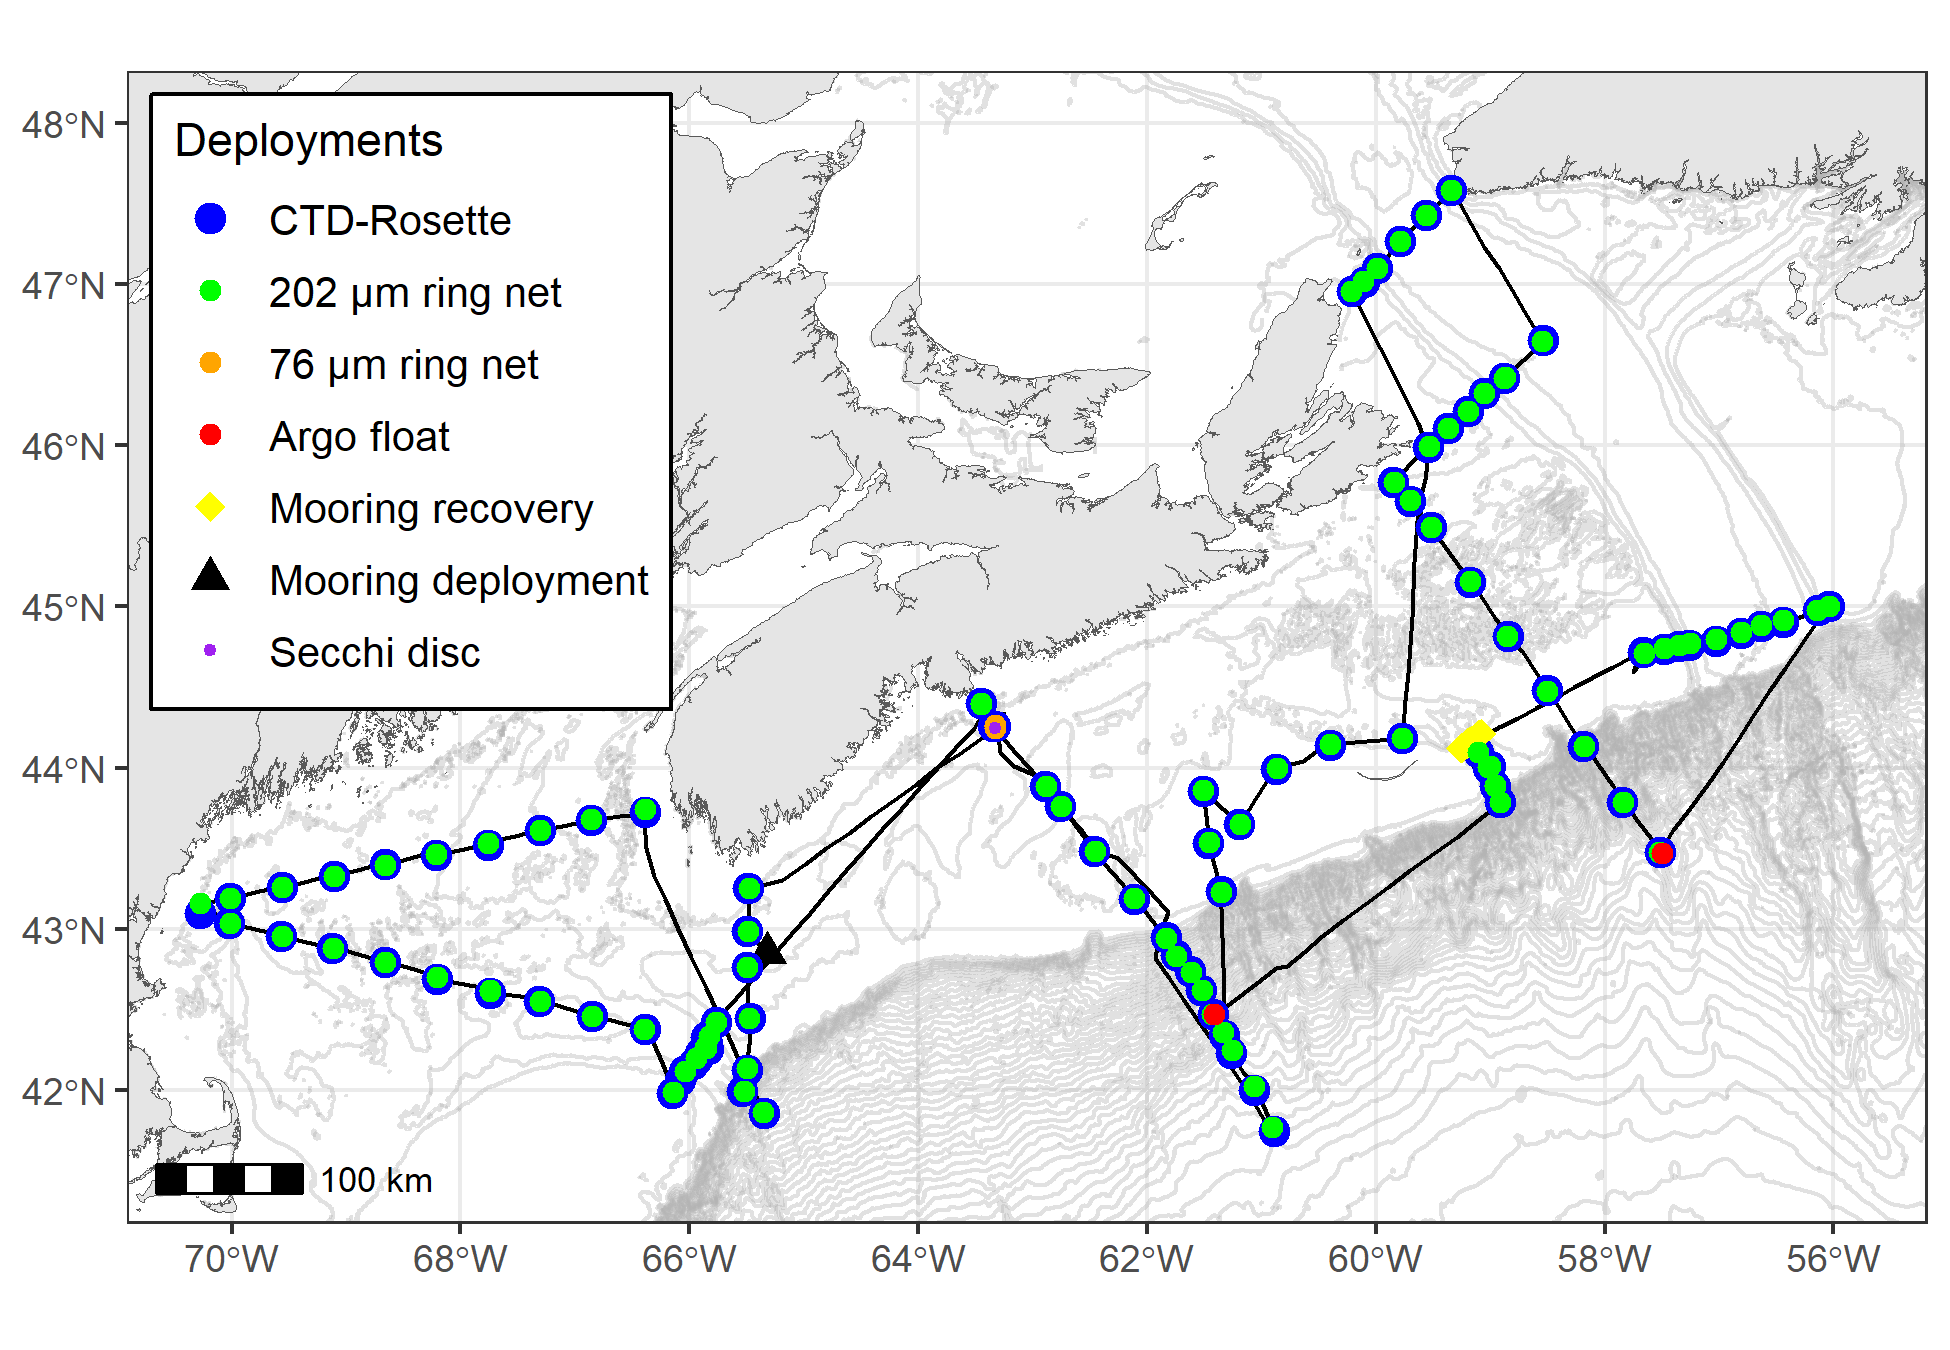
\includegraphics{knitr-figs-pdf/figure1-1} 

}

\caption{Location of stations sampled and gear deployments made during the 2025 spring AZMP mission (EN728). Note that multiple operations at single stations may not be fully reflected in the map due to overlapping labels.}\label{fig:figure1}
\end{figure}
\clearpage

\pagestyle{empty}
\begin{landscape}\begingroup\fontsize{11}{13}\selectfont
\begin{longtable}[t]{>{}l>{}l>{\raggedright\arraybackslash}m{7em}>{\raggedright\arraybackslash}m{5em}>{\raggedright\arraybackslash}m{5em}l>{\raggedright\arraybackslash}m{3em}>{\raggedright\arraybackslash}m{5em}>{\raggedright\arraybackslash}m{12em}}
\caption{\label{tab:table3}Operations conducted at each station during the 2025 spring AZMP mission (EN728), ordered sequentially by Event number. Event coordinates (in decimal degrees - DD) reflect the ship's position at the time of deployment, as recorded using the ELOG meta-data logger. Comments are associated with the 'action' on which they were entered for each event: Aborted (failed event), Deployed (gear deployment), Bottom (gear at the bottom), and Recovered (gear recovery). Note that multiple comments/actions can be present for a single event.}\\
\toprule
\begingroup\fontsize{12}{14}\selectfont \textbf{Event}\endgroup & \begingroup\fontsize{12}{14}\selectfont \textbf{Station}\endgroup & \begingroup\fontsize{12}{14}\selectfont \textbf{Gear}\endgroup & \begingroup\fontsize{12}{14}\selectfont \textbf{Start Lat. (DD)}\endgroup & \begingroup\fontsize{12}{14}\selectfont \textbf{Start Lon. (DD)}\endgroup & \begingroup\fontsize{12}{14}\selectfont \textbf{Date}\endgroup & \begingroup\fontsize{12}{14}\selectfont \textbf{Mean Depth (m)}\endgroup & \begingroup\fontsize{12}{14}\selectfont \textbf{Duration}\endgroup & \begingroup\fontsize{12}{14}\selectfont \textbf{Comments}\endgroup\\
\midrule
\endfirsthead
\caption[]{\textit{(continued)}}\\
\toprule
\begingroup\fontsize{12}{14}\selectfont \textbf{Event}\endgroup & \begingroup\fontsize{12}{14}\selectfont \textbf{Station}\endgroup & \begingroup\fontsize{12}{14}\selectfont \textbf{Gear}\endgroup & \begingroup\fontsize{12}{14}\selectfont \textbf{Start Lat. (DD)}\endgroup & \begingroup\fontsize{12}{14}\selectfont \textbf{Start Lon. (DD)}\endgroup & \begingroup\fontsize{12}{14}\selectfont \textbf{Date}\endgroup & \begingroup\fontsize{12}{14}\selectfont \textbf{Mean Depth (m)}\endgroup & \begingroup\fontsize{12}{14}\selectfont \textbf{Duration}\endgroup & \begingroup\fontsize{12}{14}\selectfont \textbf{Comments}\endgroup\\
\midrule
\endhead

\endfoot
\bottomrule
\endlastfoot
\cellcolor{ltgray}{1} & \cellcolor{ltgray}{HL\_02} & \cellcolor{ltgray}{CTD/Rosette} & \cellcolor{ltgray}{44.2565} & \cellcolor{ltgray}{-63.3269} & \cellcolor{ltgray}{2025-03-29} & \cellcolor{ltgray}{159} & \cellcolor{ltgray}{00:44:48} & \cellcolor{ltgray}{}\\
2 & HL\_02 & 202 µm net & 44.2483 & -63.3313 & 2025-03-29 & 162 & 00:12:40 & \\
\cellcolor{ltgray}{3} & \cellcolor{ltgray}{HL\_02} & \cellcolor{ltgray}{76 µm net} & \cellcolor{ltgray}{44.2460} & \cellcolor{ltgray}{-63.3315} & \cellcolor{ltgray}{2025-03-29} & \cellcolor{ltgray}{159} & \cellcolor{ltgray}{00:10:51} & \cellcolor{ltgray}{}\\
4 & HL\_02 & SECCHI DISK & 44.2437 & -63.3318 & 2025-03-29 & 158 & 00:02:34 & \\
\cellcolor{ltgray}{5} & \cellcolor{ltgray}{BBL\_01} & \cellcolor{ltgray}{202 µm net} & \cellcolor{ltgray}{43.2512} & \cellcolor{ltgray}{-65.4788} & \cellcolor{ltgray}{2025-03-30} & \cellcolor{ltgray}{64} & \cellcolor{ltgray}{00:08:52} & \cellcolor{ltgray}{}\\
6 & BBL\_01 & CTD/Rosette & 43.2538 & -65.4830 & 2025-03-30 & 63 & 00:23:32 & \\
\cellcolor{ltgray}{7} & \cellcolor{ltgray}{BBL\_02} & \cellcolor{ltgray}{202 µm net} & \cellcolor{ltgray}{42.9885} & \cellcolor{ltgray}{-65.4849} & \cellcolor{ltgray}{2025-03-30} & \cellcolor{ltgray}{119} & \cellcolor{ltgray}{00:09:07} & \cellcolor{ltgray}{}\\
8 & BBL\_02 & CTD/Rosette & 42.9883 & -65.4993 & 2025-03-30 & 116 & 00:24:03 & Recovered: 0.5 Nm south of nominal station - fishing gear on station\\
\cellcolor{ltgray}{9} & \cellcolor{ltgray}{ROBP} & \cellcolor{ltgray}{Mooring Deployment} & \cellcolor{ltgray}{42.8500} & \cellcolor{ltgray}{-65.3177} & \cellcolor{ltgray}{2025-03-30} & \cellcolor{ltgray}{148} & \cellcolor{ltgray}{00:28:25} & \cellcolor{ltgray}{In Water: CAPSULE IN WATER Other: BUBS AND ANCHOR DEPLOYED}\\
10 & BBL\_03 & 202 µm net & 42.7615 & -65.4919 & 2025-03-30 & 107 & 00:35:25 & Recovered: Submitted late\\
\cellcolor{ltgray}{11} & \cellcolor{ltgray}{BBL\_03} & \cellcolor{ltgray}{CTD/Rosette} & \cellcolor{ltgray}{42.7639} & \cellcolor{ltgray}{-65.4936} & \cellcolor{ltgray}{2025-03-30} & \cellcolor{ltgray}{107} & \cellcolor{ltgray}{00:33:03} & \cellcolor{ltgray}{}\\
12 & BBL\_04 & 202 µm net & 42.4480 & -65.4772 & 2025-03-30 & 105 & 00:07:34 & \\
\cellcolor{ltgray}{13} & \cellcolor{ltgray}{BBL\_04} & \cellcolor{ltgray}{CTD/Rosette} & \cellcolor{ltgray}{42.4463} & \cellcolor{ltgray}{-65.4713} & \cellcolor{ltgray}{2025-03-30} & \cellcolor{ltgray}{105} & \cellcolor{ltgray}{00:29:08} & \cellcolor{ltgray}{}\\
14 & BBL\_05 & 202 µm net & 42.1327 & -65.4959 & 2025-03-30 & 188 & 00:11:49 & Recovered: Poor wire angle. Could not remedy due to strong currents.\\
\cellcolor{ltgray}{15} & \cellcolor{ltgray}{BBL\_05} & \cellcolor{ltgray}{CTD/Rosette} & \cellcolor{ltgray}{42.1243} & \cellcolor{ltgray}{-65.4937} & \cellcolor{ltgray}{2025-03-30} & \cellcolor{ltgray}{240} & \cellcolor{ltgray}{00:34:09} & \cellcolor{ltgray}{Bottom: Submitted late - actual bottom time 2037}\\
16 & BBL\_06 & 202 µm net & 41.9951 & -65.5194 & 2025-03-30 & 1114 & 01:04:08 & \\
\cellcolor{ltgray}{17} & \cellcolor{ltgray}{BBL\_06} & \cellcolor{ltgray}{CTD/Rosette} & \cellcolor{ltgray}{41.9954} & \cellcolor{ltgray}{-65.5422} & \cellcolor{ltgray}{2025-03-30} & \cellcolor{ltgray}{1049} & \cellcolor{ltgray}{01:17:17} & \cellcolor{ltgray}{}\\
18 & BBL\_07 & 202 µm net & 41.8627 & -65.3523 & 2025-03-31 & 1869 & 01:12:02 & \\
\cellcolor{ltgray}{19} & \cellcolor{ltgray}{BBL\_07} & \cellcolor{ltgray}{CTD/Rosette} & \cellcolor{ltgray}{41.8552} & \cellcolor{ltgray}{-65.3461} & \cellcolor{ltgray}{2025-03-31} & \cellcolor{ltgray}{1907} & \cellcolor{ltgray}{01:45:24} & \cellcolor{ltgray}{}\\
20 & YL\_01 & 202 µm net & 43.7423 & -66.3904 & 2025-03-31 & 76 & 00:05:45 & \\
\cellcolor{ltgray}{21} & \cellcolor{ltgray}{YL\_01} & \cellcolor{ltgray}{CTD/Rosette} & \cellcolor{ltgray}{43.7266} & \cellcolor{ltgray}{-66.3868} & \cellcolor{ltgray}{2025-03-31} & \cellcolor{ltgray}{68} & \cellcolor{ltgray}{00:18:03} & \cellcolor{ltgray}{}\\
22 & YL\_02 & 202 µm net & 43.6780 & -66.8568 & 2025-03-31 & 128 & 00:09:42 & Bottom: bottom submitted late\\
\cellcolor{ltgray}{23} & \cellcolor{ltgray}{YL\_02} & \cellcolor{ltgray}{CTD/Rosette} & \cellcolor{ltgray}{43.6738} & \cellcolor{ltgray}{-66.8568} & \cellcolor{ltgray}{2025-03-31} & \cellcolor{ltgray}{126} & \cellcolor{ltgray}{00:29:16} & \cellcolor{ltgray}{}\\
24 & YL\_03 & 202 µm net & 43.6108 & -67.3052 & 2025-04-01 & 315 & 00:06:25 & Bottom: Crossbow slid partly down - net paused twice 1m below surface during recovery\\
\cellcolor{ltgray}{25} & \cellcolor{ltgray}{YL\_03} & \cellcolor{ltgray}{CTD/Rosette} & \cellcolor{ltgray}{43.6105} & \cellcolor{ltgray}{-67.3085} & \cellcolor{ltgray}{2025-04-01} & \cellcolor{ltgray}{221} & \cellcolor{ltgray}{00:37:56} & \cellcolor{ltgray}{}\\
26 & YL\_04 & 202 µm net & 43.5314 & -67.7548 & 2025-04-01 & 332 & 00:28:45 & Recovered: ring scraped ship on recovery\\
\cellcolor{ltgray}{27} & \cellcolor{ltgray}{YL\_04} & \cellcolor{ltgray}{CTD/Rosette} & \cellcolor{ltgray}{43.5218} & \cellcolor{ltgray}{-67.7551} & \cellcolor{ltgray}{2025-04-01} & \cellcolor{ltgray}{245} & \cellcolor{ltgray}{00:33:16} & \cellcolor{ltgray}{}\\
28 & YL\_05 & 202 µm net & 43.4652 & -68.2144 & 2025-04-01 & 192 & 00:16:03 & Aborted: Hit bottom. Aborted\\
\cellcolor{ltgray}{29} & \cellcolor{ltgray}{YL\_05} & \cellcolor{ltgray}{202 µm net} & \cellcolor{ltgray}{43.4622} & \cellcolor{ltgray}{-68.2155} & \cellcolor{ltgray}{2025-04-01} & \cellcolor{ltgray}{186} & \cellcolor{ltgray}{00:11:39} & \cellcolor{ltgray}{}\\
30 & YL\_05 & CTD/Rosette & 43.4550 & -68.2171 & 2025-04-01 & 189 & 00:31:01 & Recovered: sounder jumped between 192 and 182 - 182 true bottom depth\\
\cellcolor{ltgray}{31} & \cellcolor{ltgray}{YL\_06} & \cellcolor{ltgray}{202 µm net} & \cellcolor{ltgray}{43.3951} & \cellcolor{ltgray}{-68.6547} & \cellcolor{ltgray}{2025-04-01} & \cellcolor{ltgray}{149} & \cellcolor{ltgray}{00:10:41} & \cellcolor{ltgray}{}\\
32 & YL\_06 & CTD/Rosette & 43.4025 & -68.6606 & 2025-04-01 & 152 & 00:27:58 & \\
\cellcolor{ltgray}{33} & \cellcolor{ltgray}{YL\_07} & \cellcolor{ltgray}{202 µm net} & \cellcolor{ltgray}{43.3285} & \cellcolor{ltgray}{-69.1085} & \cellcolor{ltgray}{2025-04-01} & \cellcolor{ltgray}{161} & \cellcolor{ltgray}{00:05:53} & \cellcolor{ltgray}{}\\
34 & YL\_07 & CTD/Rosette & 43.3286 & -69.1049 & 2025-04-01 & 153 & 00:29:49 & \\
\cellcolor{ltgray}{35} & \cellcolor{ltgray}{YL\_08} & \cellcolor{ltgray}{202 µm net} & \cellcolor{ltgray}{43.2604} & \cellcolor{ltgray}{-69.5569} & \cellcolor{ltgray}{2025-04-01} & \cellcolor{ltgray}{152} & \cellcolor{ltgray}{00:09:24} & \cellcolor{ltgray}{}\\
36 & YL\_08 & CTD/Rosette & 43.2610 & -69.5623 & 2025-04-01 & 160 & 00:27:36 & Recovered: misfire on bottle 6 sample ID 514256\\
\cellcolor{ltgray}{37} & \cellcolor{ltgray}{YL\_09} & \cellcolor{ltgray}{202 µm net} & \cellcolor{ltgray}{43.1903} & \cellcolor{ltgray}{-70.0096} & \cellcolor{ltgray}{2025-04-02} & \cellcolor{ltgray}{108} & \cellcolor{ltgray}{00:06:52} & \cellcolor{ltgray}{}\\
38 & YL\_09 & CTD/Rosette & 43.1903 & -70.0120 & 2025-04-02 & 86 & 00:24:01 & Recovered: bottle 6 misfired sample ID 514268\\
\cellcolor{ltgray}{39} & \cellcolor{ltgray}{YL\_10} & \cellcolor{ltgray}{202 µm net} & \cellcolor{ltgray}{43.1578} & \cellcolor{ltgray}{-70.2775} & \cellcolor{ltgray}{2025-04-02} & \cellcolor{ltgray}{125} & \cellcolor{ltgray}{00:08:27} & \cellcolor{ltgray}{Recovered: twist above cod end}\\
40 & YL\_10 & CTD/Rosette & 43.0993 & -70.2791 & 2025-04-02 & 128 & 01:44:43 & Recovered: Submitted late - actual recovery time 0408 utc\\
\cellcolor{ltgray}{41} & \cellcolor{ltgray}{PL\_01} & \cellcolor{ltgray}{202 µm net} & \cellcolor{ltgray}{43.0344} & \cellcolor{ltgray}{-70.0104} & \cellcolor{ltgray}{2025-04-02} & \cellcolor{ltgray}{142} & \cellcolor{ltgray}{00:14:55} & \cellcolor{ltgray}{}\\
42 & PL\_01 & CTD/Rosette & 43.0364 & -70.0219 & 2025-04-02 & 128 & 00:26:47 & Recovered: Winkler 10m sample mis-labelled and take from surface bottle (514297; should have been 514296). Kept the sample as by the time we realized the 10m bottle had been open/exposed to atmosphere for too long to re-do the sample.\\
\cellcolor{ltgray}{43} & \cellcolor{ltgray}{PL\_02} & \cellcolor{ltgray}{202 µm net} & \cellcolor{ltgray}{42.9549} & \cellcolor{ltgray}{-69.5630} & \cellcolor{ltgray}{2025-04-02} & \cellcolor{ltgray}{166} & \cellcolor{ltgray}{00:09:21} & \cellcolor{ltgray}{}\\
44 & PL\_02 & CTD/Rosette & 42.9540 & -69.5662 & 2025-04-02 & 173 & 00:26:33 & \\
\cellcolor{ltgray}{45} & \cellcolor{ltgray}{PL\_03} & \cellcolor{ltgray}{202 µm net} & \cellcolor{ltgray}{42.8782} & \cellcolor{ltgray}{-69.1107} & \cellcolor{ltgray}{2025-04-02} & \cellcolor{ltgray}{180} & \cellcolor{ltgray}{00:19:29} & \cellcolor{ltgray}{}\\
46 & PL\_03 & CTD/Rosette & 42.8811 & -69.1191 & 2025-04-02 & 178 & 00:30:30 & \\
\cellcolor{ltgray}{47} & \cellcolor{ltgray}{PL\_04} & \cellcolor{ltgray}{202 µm net} & \cellcolor{ltgray}{42.7902} & \cellcolor{ltgray}{-68.6568} & \cellcolor{ltgray}{2025-04-02} & \cellcolor{ltgray}{204} & \cellcolor{ltgray}{00:21:16} & \cellcolor{ltgray}{}\\
48 & PL\_04 & CTD/Rosette & 42.7921 & -68.6624 & 2025-04-02 & 205 & 00:34:20 & Recovered: conductivity spike at \textasciitilde{}50m during bottle fire on the upcast - particle passed through pump and ejected on remaining upcast\\
\cellcolor{ltgray}{49} & \cellcolor{ltgray}{PL\_05} & \cellcolor{ltgray}{202 µm net} & \cellcolor{ltgray}{42.6975} & \cellcolor{ltgray}{-68.2031} & \cellcolor{ltgray}{2025-04-02} & \cellcolor{ltgray}{188} & \cellcolor{ltgray}{00:11:45} & \cellcolor{ltgray}{}\\
50 & PL\_05 & CTD/Rosette & 42.6896 & -68.2020 & 2025-04-02 & 184 & 00:29:32 & \\
\cellcolor{ltgray}{51} & \cellcolor{ltgray}{PL\_06} & \cellcolor{ltgray}{202 µm net} & \cellcolor{ltgray}{42.6212} & \cellcolor{ltgray}{-67.7446} & \cellcolor{ltgray}{2025-04-02} & \cellcolor{ltgray}{194} & \cellcolor{ltgray}{00:11:54} & \cellcolor{ltgray}{Aborted: crossbow slid down - sample kept for teaching only}\\
53 & PL\_06 & CTD/Rosette & 42.6031 & -67.7399 & 2025-04-03 & 203 & 00:35:47 & \\
\cellcolor{ltgray}{52} & \cellcolor{ltgray}{PL\_06} & \cellcolor{ltgray}{202 µm net} & \cellcolor{ltgray}{42.6119} & \cellcolor{ltgray}{-67.7381} & \cellcolor{ltgray}{2025-04-03} & \cellcolor{ltgray}{199} & \cellcolor{ltgray}{00:00:00} & \cellcolor{ltgray}{}\\
54 & PL\_07 & 202 µm net & 42.5528 & -67.3065 & 2025-04-03 & 299 & 00:20:24 & \\
\cellcolor{ltgray}{55} & \cellcolor{ltgray}{PL\_07} & \cellcolor{ltgray}{CTD/Rosette} & \cellcolor{ltgray}{42.5528} & \cellcolor{ltgray}{-67.3153} & \cellcolor{ltgray}{2025-04-03} & \cellcolor{ltgray}{301} & \cellcolor{ltgray}{00:40:14} & \cellcolor{ltgray}{}\\
56 & PL\_08 & 202 µm net & 42.4585 & -66.8502 & 2025-04-03 & 330 & 00:23:57 & \\
\cellcolor{ltgray}{57} & \cellcolor{ltgray}{PL\_08} & \cellcolor{ltgray}{CTD/Rosette} & \cellcolor{ltgray}{42.4585} & \cellcolor{ltgray}{-66.8490} & \cellcolor{ltgray}{2025-04-03} & \cellcolor{ltgray}{334} & \cellcolor{ltgray}{00:38:07} & \cellcolor{ltgray}{}\\
58 & PL\_09 & 202 µm net & 42.3782 & -66.3973 & 2025-04-03 & 269 & 00:16:19 & \\
\cellcolor{ltgray}{59} & \cellcolor{ltgray}{PL\_09} & \cellcolor{ltgray}{CTD/Rosette} & \cellcolor{ltgray}{42.3786} & \cellcolor{ltgray}{-66.3865} & \cellcolor{ltgray}{2025-04-03} & \cellcolor{ltgray}{263} & \cellcolor{ltgray}{00:36:22} & \cellcolor{ltgray}{}\\
60 & NEC\_10 & 202 µm net & 41.9832 & -66.1453 & 2025-04-03 & 94 & 00:07:28 & \\
\cellcolor{ltgray}{61} & \cellcolor{ltgray}{NEC\_10} & \cellcolor{ltgray}{CTD/Rosette} & \cellcolor{ltgray}{41.9801} & \cellcolor{ltgray}{-66.1489} & \cellcolor{ltgray}{2025-04-03} & \cellcolor{ltgray}{93} & \cellcolor{ltgray}{00:27:27} & \cellcolor{ltgray}{}\\
62 & NEC\_09 & CTD/Rosette & 42.0625 & -66.0845 & 2025-04-03 & 98 & 00:27:24 & \\
\cellcolor{ltgray}{63} & \cellcolor{ltgray}{NEC\_08} & \cellcolor{ltgray}{202 µm net} & \cellcolor{ltgray}{42.1164} & \cellcolor{ltgray}{-66.0405} & \cellcolor{ltgray}{2025-04-03} & \cellcolor{ltgray}{202} & \cellcolor{ltgray}{00:07:26} & \cellcolor{ltgray}{Recovered: time should be 1701200. hit early.}\\
64 & NEC\_08 & CTD/Rosette & 42.1158 & -66.0424 & 2025-04-03 & 207 & 00:36:04 & \\
\cellcolor{ltgray}{65} & \cellcolor{ltgray}{NEC\_07} & \cellcolor{ltgray}{CTD/Rosette} & \cellcolor{ltgray}{42.1618} & \cellcolor{ltgray}{-65.9698} & \cellcolor{ltgray}{2025-04-03} & \cellcolor{ltgray}{226} & \cellcolor{ltgray}{00:32:04} & \cellcolor{ltgray}{}\\
66 & NEC\_06 & 202 µm net & 42.1962 & -65.9373 & 2025-04-03 & 227 & 00:13:42 & \\
\cellcolor{ltgray}{67} & \cellcolor{ltgray}{NEC\_06} & \cellcolor{ltgray}{CTD/Rosette} & \cellcolor{ltgray}{42.1921} & \cellcolor{ltgray}{-65.9281} & \cellcolor{ltgray}{2025-04-03} & \cellcolor{ltgray}{230} & \cellcolor{ltgray}{00:31:23} & \cellcolor{ltgray}{}\\
68 & NEC\_05 & CTD/Rosette & 42.2306 & -65.9017 & 2025-04-03 & 239 & 00:30:10 & \\
\cellcolor{ltgray}{69} & \cellcolor{ltgray}{NEC\_04} & \cellcolor{ltgray}{202 µm net} & \cellcolor{ltgray}{42.2640} & \cellcolor{ltgray}{-65.8647} & \cellcolor{ltgray}{2025-04-03} & \cellcolor{ltgray}{228} & \cellcolor{ltgray}{00:22:26} & \cellcolor{ltgray}{Aborted: crossbow slid down}\\
70 & NEC\_04 & 202 µm net & 42.2599 & -65.8563 & 2025-04-03 & 227 & 00:17:17 & \\
\cellcolor{ltgray}{71} & \cellcolor{ltgray}{NEC\_04} & \cellcolor{ltgray}{CTD/Rosette} & \cellcolor{ltgray}{42.2504} & \cellcolor{ltgray}{-65.8347} & \cellcolor{ltgray}{2025-04-04} & \cellcolor{ltgray}{227} & \cellcolor{ltgray}{00:00:00} & \cellcolor{ltgray}{}\\
72 & NEC\_03 & CTD/Rosette & 42.2912 & -65.8436 & 2025-04-04 & 217 & 00:38:10 & \\
\cellcolor{ltgray}{73} & \cellcolor{ltgray}{NEC\_02} & \cellcolor{ltgray}{202 µm net} & \cellcolor{ltgray}{42.3307} & \cellcolor{ltgray}{-65.8302} & \cellcolor{ltgray}{2025-04-04} & \cellcolor{ltgray}{215} & \cellcolor{ltgray}{00:27:16} & \cellcolor{ltgray}{}\\
74 & NEC\_02 & CTD/Rosette & 42.3259 & -65.8521 & 2025-04-04 & 209 & 00:38:32 & \\
\cellcolor{ltgray}{75} & \cellcolor{ltgray}{NEC\_01} & \cellcolor{ltgray}{202 µm net} & \cellcolor{ltgray}{42.4219} & \cellcolor{ltgray}{-65.7634} & \cellcolor{ltgray}{2025-04-04} & \cellcolor{ltgray}{105} & \cellcolor{ltgray}{00:27:22} & \cellcolor{ltgray}{}\\
76 & NEC\_01 & CTD/Rosette & 42.4232 & -65.7687 & 2025-04-04 & 104 & 00:26:03 & Recovered: misfire on bottle 7 sample ID 514559 - this was a second 40m bottle for Dal (Bertrand) so we were conservative with water in 514558 and all samples for both DFO and Dal were able to be taken\\
\cellcolor{ltgray}{77} & \cellcolor{ltgray}{HL\_01} & \cellcolor{ltgray}{202 µm net} & \cellcolor{ltgray}{44.4007} & \cellcolor{ltgray}{-63.4495} & \cellcolor{ltgray}{2025-04-04} & \cellcolor{ltgray}{88} & \cellcolor{ltgray}{00:03:54} & \cellcolor{ltgray}{Aborted: cap fell off cod end - sample lost}\\
78 & HL\_01 & CTD/Rosette & 44.3997 & -63.4532 & 2025-04-04 & 88 & 00:26:48 & \\
\cellcolor{ltgray}{79} & \cellcolor{ltgray}{HL\_01} & \cellcolor{ltgray}{202 µm net} & \cellcolor{ltgray}{44.3938} & \cellcolor{ltgray}{-63.4490} & \cellcolor{ltgray}{2025-04-04} & \cellcolor{ltgray}{87} & \cellcolor{ltgray}{00:17:02} & \cellcolor{ltgray}{}\\
80 & HL\_02 & 202 µm net & 44.2654 & -63.3243 & 2025-04-05 & 136 & 00:10:28 & \\
\cellcolor{ltgray}{81} & \cellcolor{ltgray}{HL\_02} & \cellcolor{ltgray}{76 µm net} & \cellcolor{ltgray}{44.2631} & \cellcolor{ltgray}{-63.3301} & \cellcolor{ltgray}{2025-04-05} & \cellcolor{ltgray}{166} & \cellcolor{ltgray}{00:10:12} & \cellcolor{ltgray}{}\\
82 & HL\_02 & CTD/Rosette & 44.2577 & -63.3488 & 2025-04-05 & 161 & 00:32:00 & \\
\cellcolor{ltgray}{83} & \cellcolor{ltgray}{HL\_03} & \cellcolor{ltgray}{202 µm net} & \cellcolor{ltgray}{43.8839} & \cellcolor{ltgray}{-62.8802} & \cellcolor{ltgray}{2025-04-05} & \cellcolor{ltgray}{271} & \cellcolor{ltgray}{00:19:17} & \cellcolor{ltgray}{}\\
84 & HL\_03 & CTD/Rosette & 43.8857 & -62.8928 & 2025-04-05 & 271 & 00:37:45 & \\
\cellcolor{ltgray}{85} & \cellcolor{ltgray}{HL\_03.3} & \cellcolor{ltgray}{202 µm net} & \cellcolor{ltgray}{43.7634} & \cellcolor{ltgray}{-62.7525} & \cellcolor{ltgray}{2025-04-05} & \cellcolor{ltgray}{224} & \cellcolor{ltgray}{00:13:06} & \cellcolor{ltgray}{}\\
86 & HL\_03.3 & CTD/Rosette & 43.7644 & -62.7566 & 2025-04-05 & 212 & 00:30:50 & \\
\cellcolor{ltgray}{87} & \cellcolor{ltgray}{HL\_04} & \cellcolor{ltgray}{202 µm net} & \cellcolor{ltgray}{43.4793} & \cellcolor{ltgray}{-62.4546} & \cellcolor{ltgray}{2025-04-05} & \cellcolor{ltgray}{85} & \cellcolor{ltgray}{00:09:29} & \cellcolor{ltgray}{}\\
88 & HL\_04 & CTD/Rosette & 43.4797 & -62.4644 & 2025-04-05 & 86 & 00:24:44 & \\
\cellcolor{ltgray}{89} & \cellcolor{ltgray}{HL\_05} & \cellcolor{ltgray}{202 µm net} & \cellcolor{ltgray}{43.1877} & \cellcolor{ltgray}{-62.1108} & \cellcolor{ltgray}{2025-04-05} & \cellcolor{ltgray}{103} & \cellcolor{ltgray}{00:40:46} & \cellcolor{ltgray}{Deployed: hit deploy early by accident Recovered: Recovery hit late}\\
90 & HL\_05 & CTD/Rosette & 43.1872 & -62.1098 & 2025-04-05 & 103 & 00:17:18 & Deployed: submitted late - actual deploy time 153130\\
\cellcolor{ltgray}{91} & \cellcolor{ltgray}{HL\_05.5} & \cellcolor{ltgray}{202 µm net} & \cellcolor{ltgray}{42.9421} & \cellcolor{ltgray}{-61.8341} & \cellcolor{ltgray}{2025-04-05} & \cellcolor{ltgray}{395} & \cellcolor{ltgray}{00:25:52} & \cellcolor{ltgray}{Deployed: Sounding closer to 437 m}\\
92 & HL\_05.5 & CTD/Rosette & 42.9474 & -61.8367 & 2025-04-05 & 420 & 00:35:54 & \\
\cellcolor{ltgray}{93} & \cellcolor{ltgray}{HL\_06} & \cellcolor{ltgray}{202 µm net} & \cellcolor{ltgray}{42.8331} & \cellcolor{ltgray}{-61.7427} & \cellcolor{ltgray}{2025-04-05} & \cellcolor{ltgray}{1045} & \cellcolor{ltgray}{00:55:46} & \cellcolor{ltgray}{}\\
94 & HL\_06 & CTD/Rosette & 42.8383 & -61.7498 & 2025-04-05 & 1063 & 01:11:54 & Recovered: misfire on bottle 17 sample ID 541694 - this was the first of two 20m bottle so we were able to take from bottle 18 sample ID 541695 with careful water use to ensure all DFO and Dal samples could be taken\\
\cellcolor{ltgray}{95} & \cellcolor{ltgray}{HL\_06.3} & \cellcolor{ltgray}{202 µm net} & \cellcolor{ltgray}{42.7339} & \cellcolor{ltgray}{-61.6146} & \cellcolor{ltgray}{2025-04-06} & \cellcolor{ltgray}{1691} & \cellcolor{ltgray}{00:58:51} & \cellcolor{ltgray}{}\\
96 & HL\_06.3 & CTD/Rosette & 42.7343 & -61.6215 & 2025-04-06 & 1687 & 01:32:30 & \\
\cellcolor{ltgray}{97} & \cellcolor{ltgray}{HL\_06.7} & \cellcolor{ltgray}{202 µm net} & \cellcolor{ltgray}{42.6189} & \cellcolor{ltgray}{-61.5222} & \cellcolor{ltgray}{2025-04-06} & \cellcolor{ltgray}{2312} & \cellcolor{ltgray}{00:55:09} & \cellcolor{ltgray}{}\\
98 & HL\_06.7 & CTD/Rosette & 42.6213 & -61.5231 & 2025-04-06 & 2305 & 01:55:14 & \\
\cellcolor{ltgray}{99} & \cellcolor{ltgray}{HL\_07} & \cellcolor{ltgray}{202 µm net} & \cellcolor{ltgray}{42.4713} & \cellcolor{ltgray}{-61.4318} & \cellcolor{ltgray}{2025-04-06} & \cellcolor{ltgray}{2760} & \cellcolor{ltgray}{01:13:58} & \cellcolor{ltgray}{}\\
100 & HL\_07 & CTD/Rosette & 42.4707 & -61.4220 & 2025-04-06 & 2818 & 02:21:53 & Bottom: submitted late - actual bottom time 1015\\
\cellcolor{ltgray}{101} & \cellcolor{ltgray}{HL\_07} & \cellcolor{ltgray}{Argo float} & \cellcolor{ltgray}{42.4705} & \cellcolor{ltgray}{-61.4104} & \cellcolor{ltgray}{2025-04-06} & \cellcolor{ltgray}{2852} & \cellcolor{ltgray}{00:00:39} & \cellcolor{ltgray}{}\\
102 & GUL\_04 & 202 µm net & 43.7845 & -58.9101 & 2025-04-07 & 2074 & 01:03:59 & \\
\cellcolor{ltgray}{103} & \cellcolor{ltgray}{GUL\_04} & \cellcolor{ltgray}{CTD/Rosette} & \cellcolor{ltgray}{43.7847} & \cellcolor{ltgray}{-58.9155} & \cellcolor{ltgray}{2025-04-07} & \cellcolor{ltgray}{2217} & \cellcolor{ltgray}{01:39:22} & \cellcolor{ltgray}{Recovered: Sounding was variable - true bottom \textasciitilde{}2055}\\
104 & GUL01 & Mooring Recovery & 44.1213 & -59.2521 & 2025-04-07 & NA & 00:16:38 & \\
\cellcolor{ltgray}{105} & \cellcolor{ltgray}{GUL02} & \cellcolor{ltgray}{Mooring Recovery} & \cellcolor{ltgray}{44.1270} & \cellcolor{ltgray}{-59.2423} & \cellcolor{ltgray}{2025-04-07} & \cellcolor{ltgray}{NA} & \cellcolor{ltgray}{00:51:31} & \cellcolor{ltgray}{Aborted: Release confirmed but mooring did not release. Depth unchanged and tilt ranging between 56-58 degrees}\\
106 & GUL03 & Mooring Recovery & 44.1341 & -59.2290 & 2025-04-07 & NA & 00:33:45 & Aborted: Release confirmed but mooring did not release. Depth unchanged and tilt ranging between 68-79 degrees\\
\cellcolor{ltgray}{107} & \cellcolor{ltgray}{GUL04} & \cellcolor{ltgray}{Mooring Recovery} & \cellcolor{ltgray}{44.1424} & \cellcolor{ltgray}{-59.2142} & \cellcolor{ltgray}{2025-04-07} & \cellcolor{ltgray}{NA} & \cellcolor{ltgray}{00:21:48} & \cellcolor{ltgray}{}\\
108 & GUL05 & Mooring Recovery & 44.1487 & -59.2022 & 2025-04-07 & NA & 01:02:24 & Aborted: Communications could not be established. Moved on.\\
\cellcolor{ltgray}{109} & \cellcolor{ltgray}{GUL06} & \cellcolor{ltgray}{Mooring Recovery} & \cellcolor{ltgray}{44.1558} & \cellcolor{ltgray}{-59.1904} & \cellcolor{ltgray}{2025-04-07} & \cellcolor{ltgray}{NA} & \cellcolor{ltgray}{00:27:11} & \cellcolor{ltgray}{}\\
110 & GUL07 & Mooring Recovery & 44.1621 & -59.1772 & 2025-04-07 & NA & 00:31:30 & \\
\cellcolor{ltgray}{111} & \cellcolor{ltgray}{GUL08} & \cellcolor{ltgray}{Mooring Recovery} & \cellcolor{ltgray}{44.1664} & \cellcolor{ltgray}{-59.1631} & \cellcolor{ltgray}{2025-04-07} & \cellcolor{ltgray}{NA} & \cellcolor{ltgray}{00:14:15} & \cellcolor{ltgray}{}\\
112 & GUL09 & Mooring Recovery & 44.1735 & -59.1482 & 2025-04-07 & NA & 00:02:22 & \\
\cellcolor{ltgray}{113} & \cellcolor{ltgray}{GUL10} & \cellcolor{ltgray}{Mooring Recovery} & \cellcolor{ltgray}{44.1799} & \cellcolor{ltgray}{-59.1375} & \cellcolor{ltgray}{2025-04-07} & \cellcolor{ltgray}{200} & \cellcolor{ltgray}{00:18:14} & \cellcolor{ltgray}{}\\
114 & GUL11 & Mooring Recovery & 44.1869 & -59.1243 & 2025-04-07 & NA & 00:07:59 & \\
\cellcolor{ltgray}{115} & \cellcolor{ltgray}{GUL12} & \cellcolor{ltgray}{Mooring Recovery} & \cellcolor{ltgray}{44.1915} & \cellcolor{ltgray}{-59.1146} & \cellcolor{ltgray}{2025-04-07} & \cellcolor{ltgray}{NA} & \cellcolor{ltgray}{00:15:39} & \cellcolor{ltgray}{Aborted: Communications not established with this mooring, even after repositioning. Moved on.}\\
116 & GUL13 & Mooring Recovery & 44.1990 & -59.1038 & 2025-04-07 & NA & 00:28:10 & \\
\cellcolor{ltgray}{117} & \cellcolor{ltgray}{GUL14} & \cellcolor{ltgray}{Mooring Recovery} & \cellcolor{ltgray}{44.2061} & \cellcolor{ltgray}{-59.0934} & \cellcolor{ltgray}{2025-04-07} & \cellcolor{ltgray}{NA} & \cellcolor{ltgray}{00:35:12} & \cellcolor{ltgray}{}\\
118 & GUL15 & Mooring Recovery & 44.2104 & -59.0780 & 2025-04-07 & NA & 00:15:40 & \\
\cellcolor{ltgray}{119} & \cellcolor{ltgray}{GUL\_01} & \cellcolor{ltgray}{202 µm net} & \cellcolor{ltgray}{44.0977} & \cellcolor{ltgray}{-59.1091} & \cellcolor{ltgray}{2025-04-07} & \cellcolor{ltgray}{566} & \cellcolor{ltgray}{00:42:22} & \cellcolor{ltgray}{}\\
120 & GUL\_01 & CTD/Rosette & 44.0980 & -59.1102 & 2025-04-08 & 648 & 00:29:20 & \\
\cellcolor{ltgray}{121} & \cellcolor{ltgray}{GUL\_02} & \cellcolor{ltgray}{202 µm net} & \cellcolor{ltgray}{44.0105} & \cellcolor{ltgray}{-58.9999} & \cellcolor{ltgray}{2025-04-08} & \cellcolor{ltgray}{1181} & \cellcolor{ltgray}{01:18:34} & \cellcolor{ltgray}{}\\
122 & GUL\_02 & CTD/Rosette & 44.0092 & -59.0010 & 2025-04-08 & 1228 & 01:07:57 & \\
\cellcolor{ltgray}{123} & \cellcolor{ltgray}{GUL\_03} & \cellcolor{ltgray}{202 µm net} & \cellcolor{ltgray}{43.8881} & \cellcolor{ltgray}{-58.9548} & \cellcolor{ltgray}{2025-04-08} & \cellcolor{ltgray}{1630} & \cellcolor{ltgray}{00:56:06} & \cellcolor{ltgray}{Aborted: crossbow slid down}\\
124 & GUL\_03 & 202 µm net & 43.8888 & -58.9544 & 2025-04-08 & 1680 & 00:53:51 & \\
\cellcolor{ltgray}{125} & \cellcolor{ltgray}{GUL\_03} & \cellcolor{ltgray}{CTD/Rosette} & \cellcolor{ltgray}{43.8884} & \cellcolor{ltgray}{-58.9534} & \cellcolor{ltgray}{2025-04-08} & \cellcolor{ltgray}{1573} & \cellcolor{ltgray}{01:27:32} & \cellcolor{ltgray}{}\\
126 & GULD\_03 & 202 µm net & 44.0022 & -59.0196 & 2025-04-08 & 666 & 00:27:35 & \\
\cellcolor{ltgray}{127} & \cellcolor{ltgray}{GULD\_03} & \cellcolor{ltgray}{CTD/Rosette} & \cellcolor{ltgray}{43.9999} & \cellcolor{ltgray}{-59.0204} & \cellcolor{ltgray}{2025-04-08} & \cellcolor{ltgray}{439} & \cellcolor{ltgray}{00:39:35} & \cellcolor{ltgray}{}\\
128 & GUL12 & Mooring Recovery & 44.1931 & -59.1120 & 2025-04-08 & 245 & 00:16:08 & Attempted Comms: Re-attempting comms On Deck: Recovered successfully\\
\cellcolor{ltgray}{129} & \cellcolor{ltgray}{GUL05} & \cellcolor{ltgray}{Mooring Recovery} & \cellcolor{ltgray}{44.1491} & \cellcolor{ltgray}{-59.2035} & \cellcolor{ltgray}{2025-04-08} & \cellcolor{ltgray}{254} & \cellcolor{ltgray}{01:15:06} & \cellcolor{ltgray}{Aborted: Communications not established with this mooring or the vr4. Not recovered.}\\
130 & GUL03 & Mooring Recovery & 44.1354 & -59.2289 & 2025-04-08 & NA & 00:32:54 & Attempted Comms: Re-attempting comms Release: Status armed Aborted: Re-released mooring but the depth did not change.\\
\cellcolor{ltgray}{131} & \cellcolor{ltgray}{GUL02} & \cellcolor{ltgray}{Mooring Recovery} & \cellcolor{ltgray}{44.1285} & \cellcolor{ltgray}{-59.2426} & \cellcolor{ltgray}{2025-04-08} & \cellcolor{ltgray}{NA} & \cellcolor{ltgray}{00:09:55} & \cellcolor{ltgray}{Aborted: Status opened, but depth did not change. Aborted.}\\
132 & LCM\_01 & 202 µm net & 44.7122 & -57.6593 & 2025-04-09 & 35 & 00:01:33 & \\
\cellcolor{ltgray}{133} & \cellcolor{ltgray}{LCM\_01} & \cellcolor{ltgray}{CTD/Rosette} & \cellcolor{ltgray}{44.7167} & \cellcolor{ltgray}{-57.6608} & \cellcolor{ltgray}{2025-04-09} & \cellcolor{ltgray}{35} & \cellcolor{ltgray}{00:13:44} & \cellcolor{ltgray}{}\\
134 & LCM\_02 & 202 µm net & 44.7402 & -57.4810 & 2025-04-09 & 58 & 00:07:34 & \\
\cellcolor{ltgray}{135} & \cellcolor{ltgray}{LCM\_02} & \cellcolor{ltgray}{CTD/Rosette} & \cellcolor{ltgray}{44.7378} & \cellcolor{ltgray}{-57.4826} & \cellcolor{ltgray}{2025-04-09} & \cellcolor{ltgray}{58} & \cellcolor{ltgray}{00:16:29} & \cellcolor{ltgray}{}\\
136 & LCM\_03 & 202 µm net & 44.7593 & -57.3498 & 2025-04-09 & 68 & 00:05:35 & \\
\cellcolor{ltgray}{137} & \cellcolor{ltgray}{LCM\_03} & \cellcolor{ltgray}{CTD/Rosette} & \cellcolor{ltgray}{44.7552} & \cellcolor{ltgray}{-57.3519} & \cellcolor{ltgray}{2025-04-09} & \cellcolor{ltgray}{75} & \cellcolor{ltgray}{00:22:25} & \cellcolor{ltgray}{Recovered: misfire on bottle 1 sample ID 514866 - took bottom oxygen; pCO2; TIC; salinity samples from 60m bottle (10m difference) sample ID 514867. Samples re-labelled appropriately.}\\
138 & LCM\_04 & 202 µm net & 44.7706 & -57.2556 & 2025-04-10 & 390 & 00:10:13 & Bottom: sounding closer to 399m Recovered: missed submit for Deployed - net depolyed approx 0054 utm\\
\cellcolor{ltgray}{139} & \cellcolor{ltgray}{LCM\_04} & \cellcolor{ltgray}{CTD/Rosette} & \cellcolor{ltgray}{44.7579} & \cellcolor{ltgray}{-57.2618} & \cellcolor{ltgray}{2025-04-10} & \cellcolor{ltgray}{386} & \cellcolor{ltgray}{00:41:02} & \cellcolor{ltgray}{Recovered: misfire on bottle 7 sample ID 514883 at 50m - taking pCO2; TIC samples from 40m bottle sample ID 514884. Relabeled appropriately.}\\
140 & LCM\_05 & 202 µm net & 44.8006 & -57.0258 & 2025-04-10 & 435 & 00:25:04 & \\
\cellcolor{ltgray}{141} & \cellcolor{ltgray}{LCM\_05} & \cellcolor{ltgray}{CTD/Rosette} & \cellcolor{ltgray}{44.7885} & \cellcolor{ltgray}{-57.0256} & \cellcolor{ltgray}{2025-04-10} & \cellcolor{ltgray}{434} & \cellcolor{ltgray}{00:41:46} & \cellcolor{ltgray}{}\\
142 & LCM\_06 & 202 µm net & 44.8399 & -56.8094 & 2025-04-10 & 430 & 00:36:45 & \\
\cellcolor{ltgray}{143} & \cellcolor{ltgray}{LCM\_06} & \cellcolor{ltgray}{CTD/Rosette} & \cellcolor{ltgray}{44.8369} & \cellcolor{ltgray}{-56.8074} & \cellcolor{ltgray}{2025-04-10} & \cellcolor{ltgray}{431} & \cellcolor{ltgray}{00:39:46} & \cellcolor{ltgray}{}\\
144 & LCM\_07 & 202 µm net & 44.8847 & -56.6342 & 2025-04-10 & 422 & 00:24:18 & Recovered: weight hit bottom\\
\cellcolor{ltgray}{145} & \cellcolor{ltgray}{LCM\_07} & \cellcolor{ltgray}{CTD/Rosette} & \cellcolor{ltgray}{44.8815} & \cellcolor{ltgray}{-56.6347} & \cellcolor{ltgray}{2025-04-10} & \cellcolor{ltgray}{417} & \cellcolor{ltgray}{01:00:14} & \cellcolor{ltgray}{}\\
146 & LCM\_08 & 202 µm net & 44.9138 & -56.4393 & 2025-04-10 & 401 & 00:24:07 & \\
\cellcolor{ltgray}{147} & \cellcolor{ltgray}{LCM\_08} & \cellcolor{ltgray}{CTD/Rosette} & \cellcolor{ltgray}{44.9043} & \cellcolor{ltgray}{-56.4399} & \cellcolor{ltgray}{2025-04-10} & \cellcolor{ltgray}{400} & \cellcolor{ltgray}{00:38:49} & \cellcolor{ltgray}{Recovered: Bottle 7 misfire 514945 - no NUTS or CHL collected}\\
148 & LCM\_09 & 202 µm net & 44.9750 & -56.1448 & 2025-04-10 & 234 & 00:14:36 & \\
\cellcolor{ltgray}{149} & \cellcolor{ltgray}{LCM\_09} & \cellcolor{ltgray}{CTD/Rosette} & \cellcolor{ltgray}{44.9768} & \cellcolor{ltgray}{-56.1390} & \cellcolor{ltgray}{2025-04-10} & \cellcolor{ltgray}{213} & \cellcolor{ltgray}{00:35:39} & \cellcolor{ltgray}{Recovered: Bottle 7 misfire - 514958 - took samples from next bottle and shared with DAL (514959)}\\
150 & LCM\_10 & 202 µm net & 45.0035 & -56.0386 & 2025-04-10 & 105 & 00:06:34 & \\
\cellcolor{ltgray}{151} & \cellcolor{ltgray}{LCM\_10} & \cellcolor{ltgray}{CTD/Rosette} & \cellcolor{ltgray}{45.0001} & \cellcolor{ltgray}{-56.0360} & \cellcolor{ltgray}{2025-04-10} & \cellcolor{ltgray}{104} & \cellcolor{ltgray}{00:20:55} & \cellcolor{ltgray}{}\\
152 & LL\_09 & 202 µm net & 43.4746 & -57.5246 & 2025-04-11 & 3717 & 01:09:51 & \\
\cellcolor{ltgray}{153} & \cellcolor{ltgray}{LL\_09} & \cellcolor{ltgray}{CTD/Rosette} & \cellcolor{ltgray}{43.4739} & \cellcolor{ltgray}{-57.5169} & \cellcolor{ltgray}{2025-04-11} & \cellcolor{ltgray}{3730} & \cellcolor{ltgray}{02:39:22} & \cellcolor{ltgray}{}\\
154 & LL\_09 & Argo float & 43.4719 & -57.4984 & 2025-04-11 & 3734 & 00:05:36 & \\
\cellcolor{ltgray}{155} & \cellcolor{ltgray}{LL\_08} & \cellcolor{ltgray}{202 µm net} & \cellcolor{ltgray}{43.7846} & \cellcolor{ltgray}{-57.8390} & \cellcolor{ltgray}{2025-04-11} & \cellcolor{ltgray}{2911} & \cellcolor{ltgray}{00:56:08} & \cellcolor{ltgray}{}\\
156 & LL\_08 & CTD/Rosette & 43.7891 & -57.8457 & 2025-04-11 & 2917 & 02:10:45 & Recovered: 1 replicate of 515012 nutrients found on floor of special purpose lab - room temp for \textasciitilde{}6.5hrs. Marked with blue tape.\\
\cellcolor{ltgray}{157} & \cellcolor{ltgray}{LL\_07} & \cellcolor{ltgray}{202 µm net} & \cellcolor{ltgray}{44.1343} & \cellcolor{ltgray}{-58.1801} & \cellcolor{ltgray}{2025-04-11} & \cellcolor{ltgray}{889} & \cellcolor{ltgray}{00:41:44} & \cellcolor{ltgray}{}\\
158 & LL\_07 & CTD/Rosette & 44.1327 & -58.1879 & 2025-04-11 & 714 & 00:52:23 & Recovered: Bottle 16 misfire\\
\cellcolor{ltgray}{159} & \cellcolor{ltgray}{LL\_06} & \cellcolor{ltgray}{202 µm net} & \cellcolor{ltgray}{44.4770} & \cellcolor{ltgray}{-58.5039} & \cellcolor{ltgray}{2025-04-12} & \cellcolor{ltgray}{125} & \cellcolor{ltgray}{00:01:48} & \cellcolor{ltgray}{}\\
160 & LL\_06 & CTD/Rosette & 44.4790 & -58.5020 & 2025-04-12 & 68 & 00:18:50 & \\
\cellcolor{ltgray}{161} & \cellcolor{ltgray}{LL\_05} & \cellcolor{ltgray}{202 µm net} & \cellcolor{ltgray}{44.8170} & \cellcolor{ltgray}{-58.8499} & \cellcolor{ltgray}{2025-04-12} & \cellcolor{ltgray}{243} & \cellcolor{ltgray}{00:14:45} & \cellcolor{ltgray}{}\\
162 & LL\_05 & CTD/Rosette & 44.8161 & -58.8468 & 2025-04-12 & 249 & 00:31:46 & Bottom: flushed pumped sensors (CTD; DO) with triton between LL\_06 and LL\_05 - seems to have reduced noise in DO signal and reduced T1-T2 (better temperature could be reason for better DO).\\
\cellcolor{ltgray}{163} & \cellcolor{ltgray}{LL\_04} & \cellcolor{ltgray}{202 µm net} & \cellcolor{ltgray}{45.1568} & \cellcolor{ltgray}{-59.1763} & \cellcolor{ltgray}{2025-04-12} & \cellcolor{ltgray}{97} & \cellcolor{ltgray}{00:03:56} & \cellcolor{ltgray}{Deployed: deployed submitted late}\\
164 & LL\_04 & CTD/Rosette & 45.1540 & -59.1767 & 2025-04-12 & 107 & 00:24:11 & \\
\cellcolor{ltgray}{165} & \cellcolor{ltgray}{LL\_03} & \cellcolor{ltgray}{202 µm net} & \cellcolor{ltgray}{45.4923} & \cellcolor{ltgray}{-59.5161} & \cellcolor{ltgray}{2025-04-12} & \cellcolor{ltgray}{149} & \cellcolor{ltgray}{00:09:02} & \cellcolor{ltgray}{}\\
166 & LL\_03 & CTD/Rosette & 45.4938 & -59.5166 & 2025-04-12 & 131 & 00:25:33 & \\
\cellcolor{ltgray}{167} & \cellcolor{ltgray}{LL\_02} & \cellcolor{ltgray}{202 µm net} & \cellcolor{ltgray}{45.6580} & \cellcolor{ltgray}{-59.7017} & \cellcolor{ltgray}{2025-04-12} & \cellcolor{ltgray}{155} & \cellcolor{ltgray}{00:09:28} & \cellcolor{ltgray}{}\\
168 & LL\_02 & CTD/Rosette & 45.6556 & -59.7040 & 2025-04-12 & 144 & 00:26:11 & \\
\cellcolor{ltgray}{169} & \cellcolor{ltgray}{LL\_01} & \cellcolor{ltgray}{202 µm net} & \cellcolor{ltgray}{45.7735} & \cellcolor{ltgray}{-59.8408} & \cellcolor{ltgray}{2025-04-12} & \cellcolor{ltgray}{100} & \cellcolor{ltgray}{00:07:21} & \cellcolor{ltgray}{}\\
170 & LL\_01 & CTD/Rosette & 45.7755 & -59.8457 & 2025-04-12 & 101 & 00:23:25 & \\
\cellcolor{ltgray}{171} & \cellcolor{ltgray}{CSL\_01} & \cellcolor{ltgray}{202 µm net} & \cellcolor{ltgray}{46.9589} & \cellcolor{ltgray}{-60.2150} & \cellcolor{ltgray}{2025-04-13} & \cellcolor{ltgray}{83} & \cellcolor{ltgray}{00:07:20} & \cellcolor{ltgray}{}\\
172 & CSL\_01 & CTD/Rosette & 46.9591 & -60.2109 & 2025-04-13 & 83 & 00:22:53 & \\
\cellcolor{ltgray}{173} & \cellcolor{ltgray}{CSL\_02} & \cellcolor{ltgray}{202 µm net} & \cellcolor{ltgray}{47.0230} & \cellcolor{ltgray}{-60.1135} & \cellcolor{ltgray}{2025-04-13} & \cellcolor{ltgray}{154} & \cellcolor{ltgray}{00:12:29} & \cellcolor{ltgray}{}\\
174 & CSL\_02 & CTD/Rosette & 47.0166 & -60.1064 & 2025-04-13 & 191 & 00:29:05 & \\
\cellcolor{ltgray}{175} & \cellcolor{ltgray}{CSL\_03} & \cellcolor{ltgray}{202 µm net} & \cellcolor{ltgray}{47.0989} & \cellcolor{ltgray}{-59.9923} & \cellcolor{ltgray}{2025-04-13} & \cellcolor{ltgray}{323} & \cellcolor{ltgray}{00:19:35} & \cellcolor{ltgray}{Recovered: entered late since was deleted when the duplicate bottom entry was deleted}\\
176 & CSL\_03 & CTD/Rosette & 47.0990 & -59.9910 & 2025-04-13 & 336 & 00:38:52 & \\
\cellcolor{ltgray}{177} & \cellcolor{ltgray}{CSL\_04} & \cellcolor{ltgray}{202 µm net} & \cellcolor{ltgray}{47.2698} & \cellcolor{ltgray}{-59.7850} & \cellcolor{ltgray}{2025-04-13} & \cellcolor{ltgray}{427} & \cellcolor{ltgray}{00:27:57} & \cellcolor{ltgray}{}\\
178 & CSL\_04 & CTD/Rosette & 47.2677 & -59.7866 & 2025-04-13 & 472 & 00:42:35 & Recovered: TA/TIC sample 515173 missed and taken late (\textasciitilde{}30 mins after recovery?)\\
\cellcolor{ltgray}{179} & \cellcolor{ltgray}{CSL\_05} & \cellcolor{ltgray}{202 µm net} & \cellcolor{ltgray}{47.4295} & \cellcolor{ltgray}{-59.5587} & \cellcolor{ltgray}{2025-04-13} & \cellcolor{ltgray}{479} & \cellcolor{ltgray}{00:26:32} & \cellcolor{ltgray}{}\\
180 & CSL\_05 & CTD/Rosette & 47.4298 & -59.5591 & 2025-04-13 & 481 & 00:41:29 & \\
\cellcolor{ltgray}{181} & \cellcolor{ltgray}{CSL\_06} & \cellcolor{ltgray}{202 µm net} & \cellcolor{ltgray}{47.5838} & \cellcolor{ltgray}{-59.3404} & \cellcolor{ltgray}{2025-04-13} & \cellcolor{ltgray}{264} & \cellcolor{ltgray}{00:15:10} & \cellcolor{ltgray}{}\\
182 & CSL\_06 & CTD/Rosette & 47.5831 & -59.3400 & 2025-04-13 & 262 & 00:32:13 & \\
\cellcolor{ltgray}{183} & \cellcolor{ltgray}{STAB\_06} & \cellcolor{ltgray}{202 µm net} & \cellcolor{ltgray}{46.6476} & \cellcolor{ltgray}{-58.5446} & \cellcolor{ltgray}{2025-04-13} & \cellcolor{ltgray}{423} & \cellcolor{ltgray}{00:23:58} & \cellcolor{ltgray}{}\\
184 & STAB\_06 & CTD/Rosette & 46.6540 & -58.5422 & 2025-04-13 & 422 & 00:44:51 & \\
\cellcolor{ltgray}{185} & \cellcolor{ltgray}{STAB\_05} & \cellcolor{ltgray}{202 µm net} & \cellcolor{ltgray}{46.4181} & \cellcolor{ltgray}{-58.8807} & \cellcolor{ltgray}{2025-04-14} & \cellcolor{ltgray}{376} & \cellcolor{ltgray}{00:17:48} & \cellcolor{ltgray}{Aborted: winch wire rubbing on doghouse - paused too long at 200m}\\
186 & STAB\_05 & 202 µm net & 46.4253 & -58.8739 & 2025-04-14 & 381 & 00:22:57 & \\
\cellcolor{ltgray}{187} & \cellcolor{ltgray}{STAB\_05} & \cellcolor{ltgray}{CTD/Rosette} & \cellcolor{ltgray}{46.4168} & \cellcolor{ltgray}{-58.8811} & \cellcolor{ltgray}{2025-04-14} & \cellcolor{ltgray}{380} & \cellcolor{ltgray}{00:40:51} & \cellcolor{ltgray}{}\\
188 & STAB\_04 & 202 µm net & 46.3231 & -59.0540 & 2025-04-14 & 271 & 00:19:19 & \\
\cellcolor{ltgray}{189} & \cellcolor{ltgray}{STAB\_04} & \cellcolor{ltgray}{CTD/Rosette} & \cellcolor{ltgray}{46.3224} & \cellcolor{ltgray}{-59.0503} & \cellcolor{ltgray}{2025-04-14} & \cellcolor{ltgray}{215} & \cellcolor{ltgray}{00:31:26} & \cellcolor{ltgray}{}\\
190 & STAB\_03 & 202 µm net & 46.2156 & -59.1940 & 2025-04-14 & 96 & 00:06:26 & \\
\cellcolor{ltgray}{191} & \cellcolor{ltgray}{STAB\_03} & \cellcolor{ltgray}{CTD/Rosette} & \cellcolor{ltgray}{46.2143} & \cellcolor{ltgray}{-59.1929} & \cellcolor{ltgray}{2025-04-14} & \cellcolor{ltgray}{97} & \cellcolor{ltgray}{00:20:56} & \cellcolor{ltgray}{Recovered: raining while sampling - made effort to minimize rainwater in samples but likely not 100\%.}\\
192 & STAB\_02 & 202 µm net & 46.1085 & -59.3670 & 2025-04-14 & 76 & 00:04:44 & \\
\cellcolor{ltgray}{193} & \cellcolor{ltgray}{STAB\_02} & \cellcolor{ltgray}{CTD/Rosette} & \cellcolor{ltgray}{46.1081} & \cellcolor{ltgray}{-59.3680} & \cellcolor{ltgray}{2025-04-14} & \cellcolor{ltgray}{66} & \cellcolor{ltgray}{00:17:59} & \cellcolor{ltgray}{}\\
194 & STAB\_01 & 202 µm net & 45.9982 & -59.5357 & 2025-04-14 & 63 & 00:04:01 & \\
\cellcolor{ltgray}{195} & \cellcolor{ltgray}{STAB\_01} & \cellcolor{ltgray}{CTD/Rosette} & \cellcolor{ltgray}{45.9922} & \cellcolor{ltgray}{-59.5395} & \cellcolor{ltgray}{2025-04-14} & \cellcolor{ltgray}{59} & \cellcolor{ltgray}{00:16:58} & \cellcolor{ltgray}{}\\
196 & SIB\_11 & 202 µm net & 44.1864 & -59.7743 & 2025-04-14 & 175 & 00:11:13 & Bottom: weight kissed bottom\\
\cellcolor{ltgray}{197} & \cellcolor{ltgray}{SIB\_11} & \cellcolor{ltgray}{CTD/Rosette} & \cellcolor{ltgray}{44.1837} & \cellcolor{ltgray}{-59.7748} & \cellcolor{ltgray}{2025-04-14} & \cellcolor{ltgray}{167} & \cellcolor{ltgray}{00:30:36} & \cellcolor{ltgray}{}\\
198 & SIB\_10 & 202 µm net & 44.1440 & -60.3956 & 2025-04-15 & 146 & 00:12:58 & \\
\cellcolor{ltgray}{199} & \cellcolor{ltgray}{SIB\_10} & \cellcolor{ltgray}{CTD/Rosette} & \cellcolor{ltgray}{44.1406} & \cellcolor{ltgray}{-60.3993} & \cellcolor{ltgray}{2025-04-15} & \cellcolor{ltgray}{129} & \cellcolor{ltgray}{00:27:40} & \cellcolor{ltgray}{}\\
200 & SIB\_09 & 202 µm net & 43.9947 & -60.8649 & 2025-04-15 & 42 & 00:04:54 & \\
\cellcolor{ltgray}{201} & \cellcolor{ltgray}{SIB\_09} & \cellcolor{ltgray}{CTD/Rosette} & \cellcolor{ltgray}{43.9916} & \cellcolor{ltgray}{-60.8718} & \cellcolor{ltgray}{2025-04-15} & \cellcolor{ltgray}{45} & \cellcolor{ltgray}{00:12:20} & \cellcolor{ltgray}{}\\
202 & SIB\_05 & 202 µm net & 43.6527 & -61.1900 & 2025-04-15 & 53 & 00:06:02 & \\
\cellcolor{ltgray}{203} & \cellcolor{ltgray}{SIB\_05} & \cellcolor{ltgray}{CTD/Rosette} & \cellcolor{ltgray}{43.6507} & \cellcolor{ltgray}{-61.1931} & \cellcolor{ltgray}{2025-04-15} & \cellcolor{ltgray}{53} & \cellcolor{ltgray}{00:16:42} & \cellcolor{ltgray}{}\\
204 & SIB\_04 & 202 µm net & 43.8599 & -61.5069 & 2025-04-15 & 52 & 00:04:52 & \\
\cellcolor{ltgray}{205} & \cellcolor{ltgray}{SIB\_04} & \cellcolor{ltgray}{CTD/Rosette} & \cellcolor{ltgray}{43.8551} & \cellcolor{ltgray}{-61.5103} & \cellcolor{ltgray}{2025-04-15} & \cellcolor{ltgray}{52} & \cellcolor{ltgray}{00:15:58} & \cellcolor{ltgray}{}\\
206 & SIB\_03 & 202 µm net & 43.5383 & -61.4578 & 2025-04-15 & 60 & 00:04:57 & Deployed: 515374 missing from label stack\\
\cellcolor{ltgray}{207} & \cellcolor{ltgray}{SIB\_03} & \cellcolor{ltgray}{CTD/Rosette} & \cellcolor{ltgray}{43.5326} & \cellcolor{ltgray}{-61.4628} & \cellcolor{ltgray}{2025-04-15} & \cellcolor{ltgray}{63} & \cellcolor{ltgray}{00:16:44} & \cellcolor{ltgray}{}\\
208 & SIB\_02 & 202 µm net & 43.2304 & -61.3533 & 2025-04-15 & 120 & 00:08:00 & \\
\cellcolor{ltgray}{209} & \cellcolor{ltgray}{SIB\_02} & \cellcolor{ltgray}{CTD/Rosette} & \cellcolor{ltgray}{43.2310} & \cellcolor{ltgray}{-61.3527} & \cellcolor{ltgray}{2025-04-15} & \cellcolor{ltgray}{120} & \cellcolor{ltgray}{00:21:19} & \cellcolor{ltgray}{Recovered: Bottle 16 misfire and Bottle 12 misfire (closed but empty)}\\
210 & HL\_08 & 202 µm net & 42.3584 & -61.3389 & 2025-04-16 & 3343 & 00:55:11 & \\
\cellcolor{ltgray}{211} & \cellcolor{ltgray}{HL\_08} & \cellcolor{ltgray}{CTD/Rosette} & \cellcolor{ltgray}{42.3424} & \cellcolor{ltgray}{-61.3302} & \cellcolor{ltgray}{2025-04-16} & \cellcolor{ltgray}{3497} & \cellcolor{ltgray}{02:46:32} & \cellcolor{ltgray}{}\\
212 & HL\_09 & 202 µm net & 42.2467 & -61.2567 & 2025-04-16 & 3767 & 00:53:10 & \\
\cellcolor{ltgray}{213} & \cellcolor{ltgray}{HL\_09} & \cellcolor{ltgray}{CTD/Rosette} & \cellcolor{ltgray}{42.2262} & \cellcolor{ltgray}{-61.2664} & \cellcolor{ltgray}{2025-04-16} & \cellcolor{ltgray}{3787} & \cellcolor{ltgray}{02:52:01} & \cellcolor{ltgray}{}\\
214 & HL\_10 & 202 µm net & 42.0236 & -61.0684 & 2025-04-16 & 4082 & 00:56:03 & \\
\cellcolor{ltgray}{215} & \cellcolor{ltgray}{HL\_10} & \cellcolor{ltgray}{CTD/Rosette} & \cellcolor{ltgray}{41.9986} & \cellcolor{ltgray}{-61.0627} & \cellcolor{ltgray}{2025-04-16} & \cellcolor{ltgray}{4102} & \cellcolor{ltgray}{03:02:50} & \cellcolor{ltgray}{Recovered: Bottle 23 misfire - extra surface btl}\\
216 & HL\_11 & 202 µm net & 41.7700 & -60.9069 & 2025-04-16 & 4437 & 00:57:54 & Bottom: went deeper to remove bad wrap Recovered: Went deeper to remove bad wrap. No other chances to go this deep. Stopped on way up once to readjust spooling.\\
\cellcolor{ltgray}{217} & \cellcolor{ltgray}{HL\_11} & \cellcolor{ltgray}{CTD/Rosette} & \cellcolor{ltgray}{41.7414} & \cellcolor{ltgray}{-60.8922} & \cellcolor{ltgray}{2025-04-17} & \cellcolor{ltgray}{4454} & \cellcolor{ltgray}{00:00:00} & \cellcolor{ltgray}{}\\
218 & HL\_02 & 202 µm net & 44.2576 & -63.3257 & 2025-04-17 & 162 & 00:13:42 & \\
\cellcolor{ltgray}{219} & \cellcolor{ltgray}{HL\_02} & \cellcolor{ltgray}{76 µm net} & \cellcolor{ltgray}{44.2552} & \cellcolor{ltgray}{-63.3293} & \cellcolor{ltgray}{2025-04-17} & \cellcolor{ltgray}{156} & \cellcolor{ltgray}{00:10:41} & \cellcolor{ltgray}{}\\
220 & HL\_02 & CTD/Rosette & 44.2588 & -63.3269 & 2025-04-18 & 165 & 00:29:58 & \\*
\end{longtable}
\endgroup{}
\end{landscape}
\clearpage

\subsection{CTD-Rosette Operations}\label{ctd-operations}

\pagestyle{plain}

\subsubsection{CTD-Rosette Configuration}\label{ctd-rosette-configuration}

A 24, 10-L bottle CTD-Rosette system provided by URI was used for the duration of the EN728 mission. The CTD was configured in a steel protective cage mounted horizontally in the rosette frame. Table~\ref{tab:table4} shows a list of installed sensors on the CTD package along with their model numbers, date of last calibration, and owner. The CTD package included dual SeaBird Electronics (SBE) temperature, conductivity, and dissolved oxygen sensors, and a single Biospherical photosynthetically active radiation (PAR) sensor (rated to 2000 m), a WET Labs C-Star transmissometer, and a Valeport altimeter sensor. Two additional sensors, pH (SBE 18) and CDOM (Seapoint SUVF), were supplied by DFO's Ocean Engineering and Technology Section (OETS) for installation and use on the CTD package during the mission.

A SBE Deep SUNA nitrate sensor was mounted horizontally to the CTD cage to collect vertical profiles of nitrate and other optical parameters during the mission, representing the first Maritimes Region AZMP mission in which nitrate sensor data were collected. The sensor was connected to its own submersible battery pack mounted horizontally to the rosette frame, and was set up to log data internally (i.e., not in live mode). After each CTD cast, the data from the SUNA was downloaded separately and archived using its associated UCI software. While the Deep SUNA's depth rating is 2000 m, its corresponding battery pack was only rated to 1000 m. Consequently, both the sensor and battery pack were removed from the rosette on stations deeper than 1000 m.

\subsubsection{CTD-Rosette Deployments}\label{ctd-rosette-deployments}

Deployment of the CTD-Rosette was done using the J-frame and Winch 1 located on the starboard deck of the vessel. SBE Seasave acquisition software was operated using a shipboard acquisition computer and SBE 11 deck unit situated in the Main Laboratory. Communication between the CTD computer operator and the winch operator was done via radio. For deployments, two science staff were situated on deck to secure the rosette frame using tag lines, while a URI technician gave the hand signals to the winch operator to raise, lower, and payout the CTD-Rosette. Once the CTD-Rosette was deployed over the side and the tag lines were removed, the CTD computer operator turned on the deck unit and guided the winch operator to lower the package to 10 m depth for a 3-minute soak period, which served to trigger the pumps to turn on and allowed the sensors to acclimate. After the soak period, the CTD-Rosette was raised to the surface, and then sent on its downcast and deployed to approximately 5 m from bottom. During periods of inclement weather or high swell, the CTD package was lowered to within 7 to 10 m from the seabed.

Prior to recovery, the CTD deck unit was powered off after the surface bottles were closed. CTD-Rosette recovery procedures involved the use of gaffs and tag lines to secure the rosette frame after it breached the surface. Once on deck, the CTD-Rosette was secured using ratchet straps, and sampling of its Niskin bottles were done outside on deck.

A total of 96 CTD casts were conducted during the EN728 mission, with no aborted casts. The CTD-Rosette worked very well throughout the mission, although several bottle misfires were noted (see Table~\ref{tab:table3}. Bottles that consistently misfired were either removed from the carousel and re-positioned elsewhere, or had their trigger latch replaced (e.g., in the case of Niskin bottle \# 7). See the \hyperref[operation-issues]{Operational Considerations and Issues of Note} section below for further details.

\subsubsection{CTD Data Post-Processing}\label{ctd-data-post-processing}

Once a CTD cast was completed, the raw CTD files (.hex, .hdr, .bl, and .xmlcon) were manually copied from the CTD acquisition computer to the ship's science network where they could be accessed from any networked computer on the vessel. From here, they were copied onto BIO's post-processing computer, where the CTD Data Acquisition and Processing System (CTDDAP, Beta version 6.1), an in-house wrapper application to facilitate downloading and processing of CTD data from various SBE instruments, was used to post-process the .hex files from each cast. This allowed for the creation of ODF (Ocean Data Format) files, BIO's in-house CTD file format, and other files necessary for DFO's archival procedures. The CTD data in each ODF file was binned into 0.5 dbar bins.

A preliminary R script was written to join the nitrate data from the SUNA sensor to the CTD data using time stamps. This required reprocessing the raw CTD files without bin averaging.

\subsubsection{Water Sampling}\label{water-sampling}

Water samples were collected using 24, 10-L bottles installed on the rosette. An additional surface bottle was closed on every station in order to meet the water demands of all participants and laboratories. The number of water samples collected from each station depended on station depth and other characteristics. Standard AZMP depths (surface, 10, 20, 30, 40, 50, 60, 80, 100 m, and bottom) are consistently sampled at stations 100 m or less, while deeper bottles are typically collected at 500 m intervals (e.g., 1500, 2000 m). Water samples were processed according to standard AZMP protocols: nutrients, chlorophyll \emph{a}, dissolved oxygen, and salinity: Mitchell et al. (\citeproc{ref-Mitchell_2002}{2002}); total inorganic carbon, total alkalinity, pCO\(_2\), pH, and methane: Dickson et al. (\citeproc{ref-Dickson_2007}{2007}); particulate organic carbon and nitrogen: \url{https://www.nodc.noaa.gov/archive/arc0022/0001155/1.1/data/1-data/docs/common/proto-18.htm}; coloured-dissolved organic matter (CDOM): Mannino et al. (\citeproc{ref-Mannino_2019}{2019}); high-performance liquid chromatography (HPLC): Head and Harris (\citeproc{ref-Head_1992}{1992}); phytoplankton absorption: Hoepffner and Sathyendranath (\citeproc{ref-Hoepffner_1992}{1992}) \& Hoepffner and Sathyendranath (\citeproc{ref-Hoepffner_1993}{1993}); and flow cytometry: Li and Dickie (\citeproc{ref-Li_2001}{2001}). During occupation of AZMP high-frequency station HL\_02 on the Halifax Line, integrated phytoplankton samples were collected by collating 50 mL of water from each of the 10 bottle depths sampled, and preserving the sample using 2\% Lugol's preservative (\citeproc{ref-Mitchell_2002}{Mitchell et al. 2002}).

Sample management included the assignment of unique 6-digit `sticky IDs' to each Niskin bottle and sample vial. These IDs allow for unique identification of samples across the entire Maritimes Region AZMP timeseries. The ID range used for samples collected from the CTD-Rosette was 514025 to 515530.

\clearpage

\pagestyle{empty}
\begin{landscape}
\begin{longtable}[t]{>{\raggedright\arraybackslash}m{10em}>{\raggedright\arraybackslash}m{10em}>{\raggedright\arraybackslash}m{6em}>{\raggedright\arraybackslash}m{8em}>{\raggedright\arraybackslash}m{7em}>{\raggedright\arraybackslash}m{6em}>{\raggedright\arraybackslash}m{4em}}
\caption{\label{tab:table4}List of sensors included on the CTD system used during the 2025 spring AZMP mission on board the RV \textit{Endeavor} (EN728). Model number and date of last calibration is shown.}\\
\toprule
\begingroup\fontsize{12}{14}\selectfont \textbf{Sensor}\endgroup & \begingroup\fontsize{12}{14}\selectfont \textbf{Model}\endgroup & \begingroup\fontsize{12}{14}\selectfont \textbf{Output Parameter}\endgroup & \begingroup\fontsize{12}{14}\selectfont \textbf{QAT Output Variable Name}\endgroup & \begingroup\fontsize{12}{14}\selectfont \textbf{Serial No.}\endgroup & \begingroup\fontsize{12}{14}\selectfont \textbf{Calibration Date}\endgroup & \begingroup\fontsize{12}{14}\selectfont \textbf{Owner}\endgroup\\
\midrule
\endfirsthead
\caption[]{\textit{(continued)}}\\
\toprule
\begingroup\fontsize{12}{14}\selectfont \textbf{Sensor}\endgroup & \begingroup\fontsize{12}{14}\selectfont \textbf{Model}\endgroup & \begingroup\fontsize{12}{14}\selectfont \textbf{Output Parameter}\endgroup & \begingroup\fontsize{12}{14}\selectfont \textbf{QAT Output Variable Name}\endgroup & \begingroup\fontsize{12}{14}\selectfont \textbf{Serial No.}\endgroup & \begingroup\fontsize{12}{14}\selectfont \textbf{Calibration Date}\endgroup & \begingroup\fontsize{12}{14}\selectfont \textbf{Owner}\endgroup\\
\midrule
\endhead

\endfoot
\bottomrule
\endlastfoot
Primary CTD deck unit & SBE 11plus & NA & NA & NA & NA & URI\\
CTD underwater unit & SBE 9plus & NA & NA & NA & NA & URI\\
Primary temperature & SBE 3P & ITS-90 temperature, Celcius & t090C & 4695 & 2024-01-17 & URI\\
Primary conductivity & SBE 4C & Conductivity, S/m & c0S/m & 618 & 2024-01-23 & URI\\
Digiquartz pressure sensor & Paroscientific & dbar & prDM & 444 & 2024-03-21 & URI\\
Primary dissolved oxygen & SBE 43 & Dissolved oxygen, ml/l & sbeox0 & 1648 & 2024-08-09 & URI\\
Secondary temperature & SBE 3P & ITS-90 temperature, Celcius & t191C & 4130 & 2024-01-18 & URI\\
Secondary conductivity & SBE 4C & Conductivity, S/m & c1S/m & 2822 & 2024-01-23 & URI\\
Secondary dissolved oxygen & SBE 43 & Dissolved oxygen, ml/l & sbeox1 & 4281 & 2024-07-11 & URI\\
pH & SBE 18 & NA & ph & 1251 & 2025-03-06 & DFO\\
Chlorophyll fluorometer & Wet Labs ECO AFL/FL & micro g/L & flSP & 4028 & 2023-12-18 & URI\\
CDOM fluorometer & Seapoint Fluorometer SCF & micro g/L & flSPuv0 & 6225 & 2025-03-07 & DFO\\
PAR/Log & Biospherical Licor Chelsea Sensor & micromoles photons/m2/s & par & 70709 & 2023-06-07 & URI\\
Nitrate & Deep SUNA & milligrams/L & NA & NTR-2382 & 2024-10-17 & DFO\\
Transmissometer & WET Labs C-Star & Beam attenuation (1/m), Beam transmission (\%) & CStarAt0 & 969DR & 2024-02-23 & URI\\
Altimeter & Valeport VA500 & metres & altM & 49898 & 2015-03-30 & URI\\*
\end{longtable}
\end{landscape}
\clearpage

\pagestyle{plain}

Table~\ref{tab:table5} shows the total number of samples collected for each parameter measured and evaluated by the AZMP from CTD-Rosette deployments at each station. Bottle samples collected for salinity determination were analyzed at sea using a DFO-owned Guildline Autosal 8410A Salinometer set up in the Special Purpose Laboratory. As the temperature seemed to fluctuate in this lab, salinity samples were analyzed with the door closed and air conditioning set to 23\(^\circ\)C to promote a consistent temperature and high-quality measurements.

Dissolved oxygen samples were titrated and analyzed at sea after being stored in the fridge for several hours using a modified Winkler technique with automated electrical endpoint system, while chlorophyll samples were analyzed using a Turner Designs fluorometer after being stored for at least 24 hours in a -20\(^\circ\)C freezer. Samples collected for all other parameters were either stored at room temperature, refrigerated, or frozen for subsequent analysis ashore.

\subsubsection{Data Accessibility}\label{data-accessibility}

Upon completion of this mission, the CTD data will undergo various quality control checks to correct metadata errors and/or erroneous CTD values (e.g., data spikes), and the primary and secondary conductivity and oxygen sensor data will be calibrated using bottle measurements following SeaBird's `Computing Temperature \& Conductivity Slope \& Offset Correction Coefficients from Lab Calibration and Salinity Bottle Samples' \link{https://www.seabird.com/sbe-4-conductivity-sensor/product-downloads?id=60762467707}{Application Note No.~31} (\citeproc{ref-SBE_2024a}{Scientific 2024a}) and `SBE 43 Dissolved Oxygen Sensor Calibration and Data Corrections' \link{https://www.seabird.com/oxygen-sensors/sbe-43-dissolved-oxygen-sensor/family-downloads?productCategoryId=54627869932}{Application Note No.~64-2} (\citeproc{ref-SBE_2024b}{Scientific 2024b}); also described in Beazley et al. (\citeproc{ref-Beazley_2024}{2024})). These final calibrated files are available in .ODF format by request to \link{mailto:DFO.BIODataServices-BIOServicesdeDonnees.MPO@dfo-mpo.gc.ca}{\nolinkurl{DFO.BIODataServices-BIOServicesdeDonnees.MPO@dfo-mpo.gc.ca}}, or can be downloaded directly in netCDF or other common formats from the Canadian Integrated Ocean Observing System (CIOOS) \link{https://catalogue.cioos.ca/dataset/ca-cioos_9a4bd73f-12a2-40ff-a7c7-b961a1d113111}{ERDDAP}.

Bottle measurements can be extracted from DFO's national repository for discrete bottle and plankton data, \link{https://www.dfo-mpo.gc.ca/science/data-donnees/biochem/index-eng.html}{BioChem}, or can be made available by request to \link{mailto:DFO.BIODataServices-BIOServicesdeDonnees.MPO@dfo-mpo.gc.ca}{\nolinkurl{DFO.BIODataServices-BIOServicesdeDonnees.MPO@dfo-mpo.gc.ca}}.

\clearpage

\pagestyle{empty}
\begin{landscape}
\begin{longtable}[t]{lllllllll>{\raggedright\arraybackslash}p{3em}lll}
\caption{\label{tab:table5}Summary of water samples collected for each parameter sampled on the 2025 spring AZMP mission (EN728). Numbers represent the total number of samples per station, where O\textsubscript{2} = dissolved oxygen, pCO\textsubscript{2} = partial pressure of carbon dioxide, TIC/TA = total inorganic carbon and total alkalinity, NUTS = nutrients, SAL = salinity, CHL = chlorophyll, POC = particulate organic carbon, HPLC = high performance liquid chromatography, ABS = phytoplankton absorption, CDOM = coloured dissolved organic matter, and CYTO = flow cytometry.}\\
\toprule
\begingroup\fontsize{12}{14}\selectfont \textbf{Station}\endgroup & \begingroup\fontsize{12}{14}\selectfont \textbf{Event}\endgroup & \begingroup\fontsize{12}{14}\selectfont \textbf{O2}\endgroup & \begingroup\fontsize{12}{14}\selectfont \textbf{pCO2}\endgroup & \begingroup\fontsize{12}{14}\selectfont \textbf{TIC/TA}\endgroup & \begingroup\fontsize{12}{14}\selectfont \textbf{NUTS}\endgroup & \begingroup\fontsize{12}{14}\selectfont \textbf{SAL}\endgroup & \begingroup\fontsize{12}{14}\selectfont \textbf{CHL}\endgroup & \begingroup\fontsize{12}{14}\selectfont \textbf{POC/ PON}\endgroup & \begingroup\fontsize{12}{14}\selectfont \textbf{HPLC}\endgroup & \begingroup\fontsize{12}{14}\selectfont \textbf{ABS}\endgroup & \begingroup\fontsize{12}{14}\selectfont \textbf{CDOM}\endgroup & \begingroup\fontsize{12}{14}\selectfont \textbf{CYTO}\endgroup\\
\midrule
\endfirsthead
\caption[]{\textit{(continued)}}\\
\toprule
\begingroup\fontsize{12}{14}\selectfont \textbf{Station}\endgroup & \begingroup\fontsize{12}{14}\selectfont \textbf{Event}\endgroup & \begingroup\fontsize{12}{14}\selectfont \textbf{O2}\endgroup & \begingroup\fontsize{12}{14}\selectfont \textbf{pCO2}\endgroup & \begingroup\fontsize{12}{14}\selectfont \textbf{TIC/TA}\endgroup & \begingroup\fontsize{12}{14}\selectfont \textbf{NUTS}\endgroup & \begingroup\fontsize{12}{14}\selectfont \textbf{SAL}\endgroup & \begingroup\fontsize{12}{14}\selectfont \textbf{CHL}\endgroup & \begingroup\fontsize{12}{14}\selectfont \textbf{POC/ PON}\endgroup & \begingroup\fontsize{12}{14}\selectfont \textbf{HPLC}\endgroup & \begingroup\fontsize{12}{14}\selectfont \textbf{ABS}\endgroup & \begingroup\fontsize{12}{14}\selectfont \textbf{CDOM}\endgroup & \begingroup\fontsize{12}{14}\selectfont \textbf{CYTO}\endgroup\\
\midrule
\endhead

\endfoot
\bottomrule
\endlastfoot
HL\_02 & 1 & 3 & 6 & 6 & 20 & 2 & 18 & 2 & 2 & 2 & 2 & 18\\
BBL\_01 & 6 & 3 & 4 & 4 & 14 & 2 & 14 & 2 & 2 & 2 & 2 & 14\\
BBL\_02 & 8 & 3 & 0 & 0 & 18 & 2 & 18 & 2 & 1 & 1 & 1 & 18\\
BBL\_03 & 11 & 3 & 5 & 5 & 18 & 2 & 18 & 2 & 2 & 2 & 2 & 18\\
BBL\_04 & 13 & 3 & 0 & 0 & 18 & 2 & 18 & 2 & 1 & 1 & 1 & 18\\
BBL\_05 & 15 & 3 & 6 & 6 & 22 & 2 & 18 & 2 & 2 & 2 & 2 & 18\\
BBL\_06 & 17 & 4 & 9 & 9 & 30 & 3 & 18 & 2 & 1 & 1 & 1 & 20\\
BBL\_07 & 19 & 5 & 11 & 11 & 32 & 4 & 18 & 2 & 2 & 2 & 2 & 24\\
YL\_01 & 21 & 3 & 5 & 5 & 16 & 2 & 16 & 2 & 1 & 1 & 1 & 16\\
YL\_02 & 23 & 3 & 0 & 0 & 20 & 2 & 18 & 2 & 1 & 1 & 1 & 18\\
YL\_03 & 25 & 3 & 7 & 7 & 22 & 2 & 18 & 2 & 1 & 1 & 1 & 18\\
YL\_04 & 27 & 3 & 0 & 0 & 22 & 2 & 18 & 2 & 1 & 1 & 1 & 18\\
YL\_05 & 30 & 3 & 7 & 7 & 22 & 2 & 18 & 2 & 1 & 1 & 1 & 18\\
YL\_06 & 32 & 3 & 0 & 0 & 20 & 2 & 18 & 2 & 1 & 1 & 1 & 18\\
YL\_07 & 34 & 3 & 6 & 6 & 20 & 2 & 18 & 2 & 1 & 1 & 1 & 18\\
YL\_08 & 36 & 3 & 6 & 6 & 25 & 2 & 16 & 2 & 1 & 1 & 1 & 18\\
YL\_09 & 38 & 3 & 0 & 0 & 21 & 2 & 14 & 2 & 1 & 1 & 1 & 0\\
YL\_10 & 40 & 3 & 5 & 5 & 18 & 2 & 18 & 2 & 1 & 1 & 1 & 18\\
PL\_01 & 42 & 3 & 5 & 5 & 20 & 2 & 18 & 2 & 1 & 1 & 1 & 0\\
PL\_02 & 44 & 3 & 0 & 0 & 20 & 2 & 18 & 2 & 1 & 1 & 1 & 0\\
PL\_03 & 46 & 3 & 7 & 7 & 22 & 2 & 18 & 2 & 1 & 1 & 1 & 0\\
PL\_04 & 48 & 3 & 0 & 0 & 22 & 2 & 18 & 2 & 1 & 1 & 1 & 0\\
PL\_05 & 50 & 3 & 6 & 6 & 20 & 2 & 18 & 2 & 1 & 1 & 1 & 0\\
PL\_06 & 53 & 3 & 0 & 0 & 22 & 2 & 18 & 2 & 1 & 1 & 1 & 0\\
PL\_07 & 55 & 4 & 8 & 8 & 24 & 3 & 18 & 2 & 1 & 1 & 1 & 0\\
PL\_08 & 57 & 4 & 0 & 0 & 24 & 3 & 18 & 2 & 1 & 1 & 1 & 0\\
PL\_09 & 59 & 4 & 7 & 7 & 24 & 3 & 18 & 2 & 1 & 1 & 1 & 0\\
NEC\_10 & 61 & 3 & 0 & 0 & 18 & 2 & 18 & 2 & 1 & 1 & 1 & 0\\
NEC\_09 & 62 & 3 & 5 & 5 & 18 & 2 & 0 & 0 & 0 & 0 & 0 & 0\\
NEC\_08 & 64 & 3 & 0 & 0 & 26 & 2 & 18 & 2 & 1 & 1 & 1 & 0\\
NEC\_07 & 65 & 3 & 7 & 7 & 26 & 2 & 0 & 0 & 0 & 0 & 0 & 0\\
NEC\_06 & 67 & 3 & 0 & 0 & 26 & 2 & 18 & 2 & 1 & 1 & 1 & 0\\
NEC\_05 & 68 & 3 & 6 & 6 & 26 & 2 & 0 & 0 & 0 & 0 & 0 & 0\\
NEC\_04 & 71 & 3 & 0 & 0 & 26 & 2 & 18 & 2 & 1 & 1 & 1 & 0\\
NEC\_03 & 72 & 3 & 6 & 6 & 26 & 2 & 0 & 0 & 0 & 0 & 0 & 0\\
NEC\_02 & 74 & 3 & 6 & 6 & 26 & 2 & 0 & 0 & 0 & 0 & 0 & 0\\
NEC\_01 & 76 & 3 & 0 & 0 & 18 & 2 & 18 & 2 & 1 & 1 & 1 & 0\\
HL\_01 & 78 & 3 & 5 & 5 & 16 & 2 & 16 & 2 & 1 & 1 & 1 & 14\\
HL\_02 & 82 & 3 & 6 & 6 & 20 & 2 & 18 & 2 & 2 & 2 & 2 & 18\\
HL\_03 & 84 & 3 & 7 & 7 & 22 & 2 & 18 & 2 & 1 & 1 & 1 & 18\\
HL\_03.3 & 86 & 3 & 0 & 0 & 20 & 2 & 18 & 2 & 2 & 2 & 2 & 0\\
HL\_04 & 88 & 3 & 5 & 5 & 16 & 2 & 16 & 2 & 1 & 1 & 1 & 14\\
HL\_05 & 90 & 3 & 5 & 5 & 18 & 2 & 18 & 2 & 2 & 2 & 2 & 18\\
HL\_05.5 & 92 & 4 & 7 & 7 & 22 & 3 & 18 & 2 & 1 & 1 & 1 & 0\\
HL\_06 & 94 & 9 & 11 & 11 & 30 & 8 & 18 & 2 & 2 & 2 & 2 & 20\\
HL\_06.3 & 96 & 6 & 0 & 0 & 32 & 5 & 18 & 2 & 1 & 1 & 1 & 0\\
HL\_06.7 & 98 & 12 & 0 & 0 & 34 & 11 & 18 & 2 & 1 & 1 & 1 & 0\\
HL\_07 & 100 & 12 & 13 & 13 & 34 & 11 & 18 & 2 & 2 & 2 & 2 & 20\\
GUL\_04 & 103 & 4 & 6 & 6 & 28 & 3 & 19 & 2 & 1 & 1 & 1 & 18\\
GUL\_01 & 120 & 4 & 1 & 1 & 24 & 3 & 18 & 2 & 1 & 1 & 1 & 18\\
GUL\_02 & 122 & 4 & 1 & 1 & 26 & 3 & 18 & 2 & 1 & 1 & 1 & 18\\
GUL\_03 & 125 & 4 & 2 & 2 & 28 & 3 & 18 & 2 & 1 & 1 & 1 & 18\\
GULD\_03 & 127 & 4 & 1 & 1 & 22 & 3 & 18 & 2 & 1 & 1 & 1 & 0\\
LCM\_01 & 133 & 3 & 3 & 3 & 8 & 2 & 8 & 2 & 1 & 1 & 1 & 0\\
LCM\_02 & 135 & 3 & 0 & 0 & 12 & 2 & 12 & 2 & 1 & 1 & 1 & 0\\
LCM\_03 & 135 & 3 & 2 & 2 & 14 & 2 & 14 & 2 & 2 & 2 & 2 & 0\\
LCM\_04 & 139 & 3 & 6 & 6 & 20 & 2 & 16 & 2 & 1 & 1 & 1 & 0\\
LCM\_05 & 141 & 3 & 6 & 6 & 22 & 2 & 18 & 2 & 2 & 2 & 2 & 0\\
LCM\_06 & 143 & 3 & 0 & 0 & 22 & 2 & 18 & 2 & 1 & 1 & 1 & 0\\
LCM\_07 & 145 & 4 & 5 & 5 & 22 & 2 & 18 & 2 & 2 & 2 & 2 & 0\\
LCM\_08 & 147 & 4 & 0 & 0 & 22 & 2 & 18 & 2 & 1 & 1 & 1 & 0\\
LCM\_09 & 149 & 3 & 5 & 5 & 20 & 2 & 18 & 2 & 2 & 2 & 2 & 0\\
LCM\_10 & 151 & 3 & 4 & 4 & 18 & 2 & 17 & 2 & 1 & 1 & 1 & 0\\
LL\_09 & 153 & 5 & 12 & 12 & 34 & 4 & 18 & 2 & 2 & 2 & 2 & 20\\
LL\_08 & 157 & 4 & 10 & 10 & 32 & 4 & 18 & 2 & 1 & 1 & 1 & 0\\
LL\_07 & 158 & 4 & 7 & 7 & 26 & 3 & 18 & 2 & 2 & 2 & 2 & 18\\
LL\_06 & 160 & 3 & 0 & 0 & 14 & 2 & 14 & 2 & 1 & 1 & 1 & 14\\
LL\_05 & 162 & 3 & 7 & 7 & 20 & 2 & 18 & 2 & 2 & 2 & 2 & 18\\
LL\_04 & 164 & 3 & 7 & 7 & 18 & 2 & 16 & 2 & 1 & 1 & 1 & 17\\
LL\_03 & 166 & 3 & 7 & 7 & 20 & 2 & 18 & 2 & 2 & 2 & 2 & 18\\
LL\_02 & 168 & 3 & 7 & 7 & 20 & 2 & 18 & 2 & 1 & 1 & 1 & 18\\
LL\_01 & 170 & 3 & 6 & 6 & 18 & 2 & 18 & 2 & 2 & 2 & 2 & 18\\
CSL\_01 & 172 & 3 & 6 & 6 & 16 & 2 & 16 & 2 & 2 & 2 & 2 & 16\\
CSL\_02 & 174 & 3 & 8 & 8 & 22 & 2 & 18 & 2 & 1 & 1 & 1 & 18\\
CSL\_03 & 176 & 4 & 10 & 10 & 26 & 3 & 18 & 2 & 2 & 2 & 2 & 18\\
CSL\_04 & 178 & 4 & 11 & 11 & 28 & 3 & 18 & 2 & 1 & 1 & 1 & 18\\
CSL\_06 & 182 & 3 & 9 & 9 & 24 & 2 & 18 & 2 & 1 & 1 & 1 & 18\\
STAB\_06 & 184 & 3 & 0 & 0 & 26 & 2 & 18 & 2 & 1 & 1 & 1 & 0\\
STAB\_05 & 187 & 3 & 2 & 2 & 26 & 2 & 18 & 2 & 1 & 1 & 1 & 0\\
STAB\_04 & 189 & 3 & 0 & 0 & 22 & 2 & 18 & 2 & 1 & 1 & 1 & 0\\
STAB\_03 & 191 & 3 & 2 & 2 & 16 & 2 & 16 & 2 & 1 & 1 & 1 & 0\\
STAB\_02 & 193 & 3 & 0 & 0 & 14 & 2 & 14 & 2 & 1 & 1 & 1 & 0\\
STAB\_01 & 195 & 3 & 1 & 1 & 12 & 2 & 12 & 2 & 1 & 1 & 1 & 0\\
SIB\_11 & 197 & 3 & 2 & 3 & 18 & 2 & 18 & 2 & 1 & 1 & 1 & 10\\
SIB\_10 & 199 & 3 & 0 & 0 & 18 & 2 & 18 & 4 & 2 & 2 & 2 & 10\\
SIB\_09 & 201 & 3 & 2 & 2 & 10 & 2 & 10 & 2 & 1 & 1 & 1 & 6\\
SIB\_05 & 203 & 3 & 0 & 0 & 12 & 2 & 12 & 2 & 1 & 1 & 1 & 8\\
SIB\_04 & 205 & 3 & 2 & 2 & 12 & 2 & 12 & 4 & 2 & 2 & 2 & 8\\
SIB\_03 & 207 & 3 & 0 & 0 & 14 & 2 & 14 & 2 & 1 & 1 & 1 & 8\\
SIB\_02 & 209 & 3 & 0 & 2 & 16 & 2 & 18 & 4 & 2 & 2 & 2 & 10\\
HL\_08 & 211 & 17 & 0 & 0 & 34 & 15 & 18 & 2 & 1 & 1 & 1 & 10\\
HL\_09 & 213 & 18 & 0 & 0 & 35 & 17 & 18 & 2 & 1 & 1 & 1 & 10\\
HL\_10 & 215 & 17 & 0 & 0 & 36 & 16 & 18 & 2 & 1 & 1 & 1 & 10\\
HL\_11 & 217 & 78 & 0 & 0 & 48 & 17 & 18 & 2 & 1 & 1 & 1 & 10\\
HL\_02 & 220 & 3 & 6 & 6 & 20 & 2 & 18 & 2 & 2 & 2 & 2 & 18\\*
\end{longtable}
\end{landscape}
\clearpage

\pagestyle{plain}

\subsection{Vertical Ring Net Tows}\label{vertical-ring-net-tows}

At each station, a conical ring net with an aperture of 75 cm and rigged with 202 µm mesh (filtering ratio of 1:5) was towed vertically from near-bottom to the surface (or to a maximum of 1000 m) to collect samples used by the AZMP to describe changes in mesozooplankton abundance and biomass across the Scotian Shelf. Ring net operations were conducted from the vessel's J-frame using the secondary three-conductor electromechanical (EM) cable and winch (termed `Winch 2'). The diameter of this cable was 0.322'' (\textasciitilde8 mm) and required crossbows compatible with a thicker-gauge wire. A 220 lb weight was shackled to the termination of this cable and was designed to keep the net straight in the water column during deployment.

Standard operating procedures were to deploy the ring net system at a speed of 30 m/min to within 10 m from the seabed based on total water column depth, and then recover the system at a rate of 50 m/min without slowing or stopping until the top of the net was out of the water. Ring nets were equipped with a KC Denmark flow meter, which was used to record the start and end flow for each cast. The net was gently rinsed using a seawater hose, and the contents of the code end was preserved in 4\% buffered formaldehyde (10\% formalin). Net operations at station HL\_02 consisted of the standard (202 µm) net deployment, and a 76 µm net deployment preserved in formalin.

A total of 101 ring net operations were conducted at 90 unique stations during the mission (see Table~\ref{tab:table3}), including a total of 3, 76 µm net deployments at station HL\_02. An angle finder was used to assess wire angle during the net ascent, and typically ranged between 5 and 15\(^\circ\). The ring net tow at station YL\_05 (Event 028) was aborted after the net hit the bottom, at stations PL\_06 (Event 051), NEC\_04 (Event 069), and GUL\_03 (Event 123), ring net operations were aborted and re-deployed after the crossbow slid down the wire. This issue is described further in the \hyperref[operation-issues]{Operational Considerations and Issues of Note} section below. At station HL\_01 (Event 077) was aborted after the end cap fell off the cod end, and the sample was lost. This cod end was quickly replaced after the net was washed down, and the net was redeployed. At station STAB\_05 (Event 185), the net was aborted after the cable started to rub up against the winch house after the winch was adjusted. The winch was adjusted again and the net re-deployed successfully.

\subsubsection{Data Accessibility}\label{data-accessibility-1}

The wet biomass of large (\textgreater{} 10 mm) and small (\textless{} 10 mm) zooplankton (separate and combined), the dry weight of small zooplankton, and abundances of large zooplankton taxa and a sub-sample of small zooplankton taxa will be uploaded and available in BioChem upon completion of the analysis of samples in the laboratory, and can also be provided upon request to \link{mailto:DFO.BIODataServices-BIOServicesdeDonnees.MPO@dfo-mpo.gc.ca}{\nolinkurl{DFO.BIODataServices-BIOServicesdeDonnees.MPO@dfo-mpo.gc.ca}}.

\clearpage

\subsection{Argo Floats}\label{argo-floats}

During the EN728 mission, DFO deployed 2 Argo floats from the RV \emph{Endeavor} in support of the international \link{https://argo.ucsd.edu/}{Argo program} (\citeproc{ref-wong2020}{Wong et al. 2020}). Both floats were NKE ARVOR core float models, which record temperature, conductivity, and depth. The first float was deployed at station HL\_07 after completion of the CTD and ring net operations there. The second float was deployed at station LL\_09, also following CTD and ring net operations. The location of each deployment can be seen in Figure~\ref{fig:figure2}.

Both floats were deployed by hand by two crew using a slip line from the aft starboard deck while the ship was underway doing 1-2 kts. One hour prior to deployment, the floats were pre-tested to confirm establishment of the float's GPS and iridium communications. The floats will remain active for approximately 5 years, collecting vertical profiles from the surface to 2000 m every 10 days.

The first profile recorded by each float is shown in Figure~\ref{fig:figure3}. This profile was collected during ascent of the float, approximately 2 days after deployment. Salinity sensor data from the floats were compared with bottle salinity measurements collected on the CTD casts (up to a depth of 2000 m) from nearby stations HL07 and LL\_09 (Figure~\ref{fig:figure3}), and were found to be consistent.

\hspace*{-0.2in}
\begin{figure}[htb]

{\centering \pdftooltip{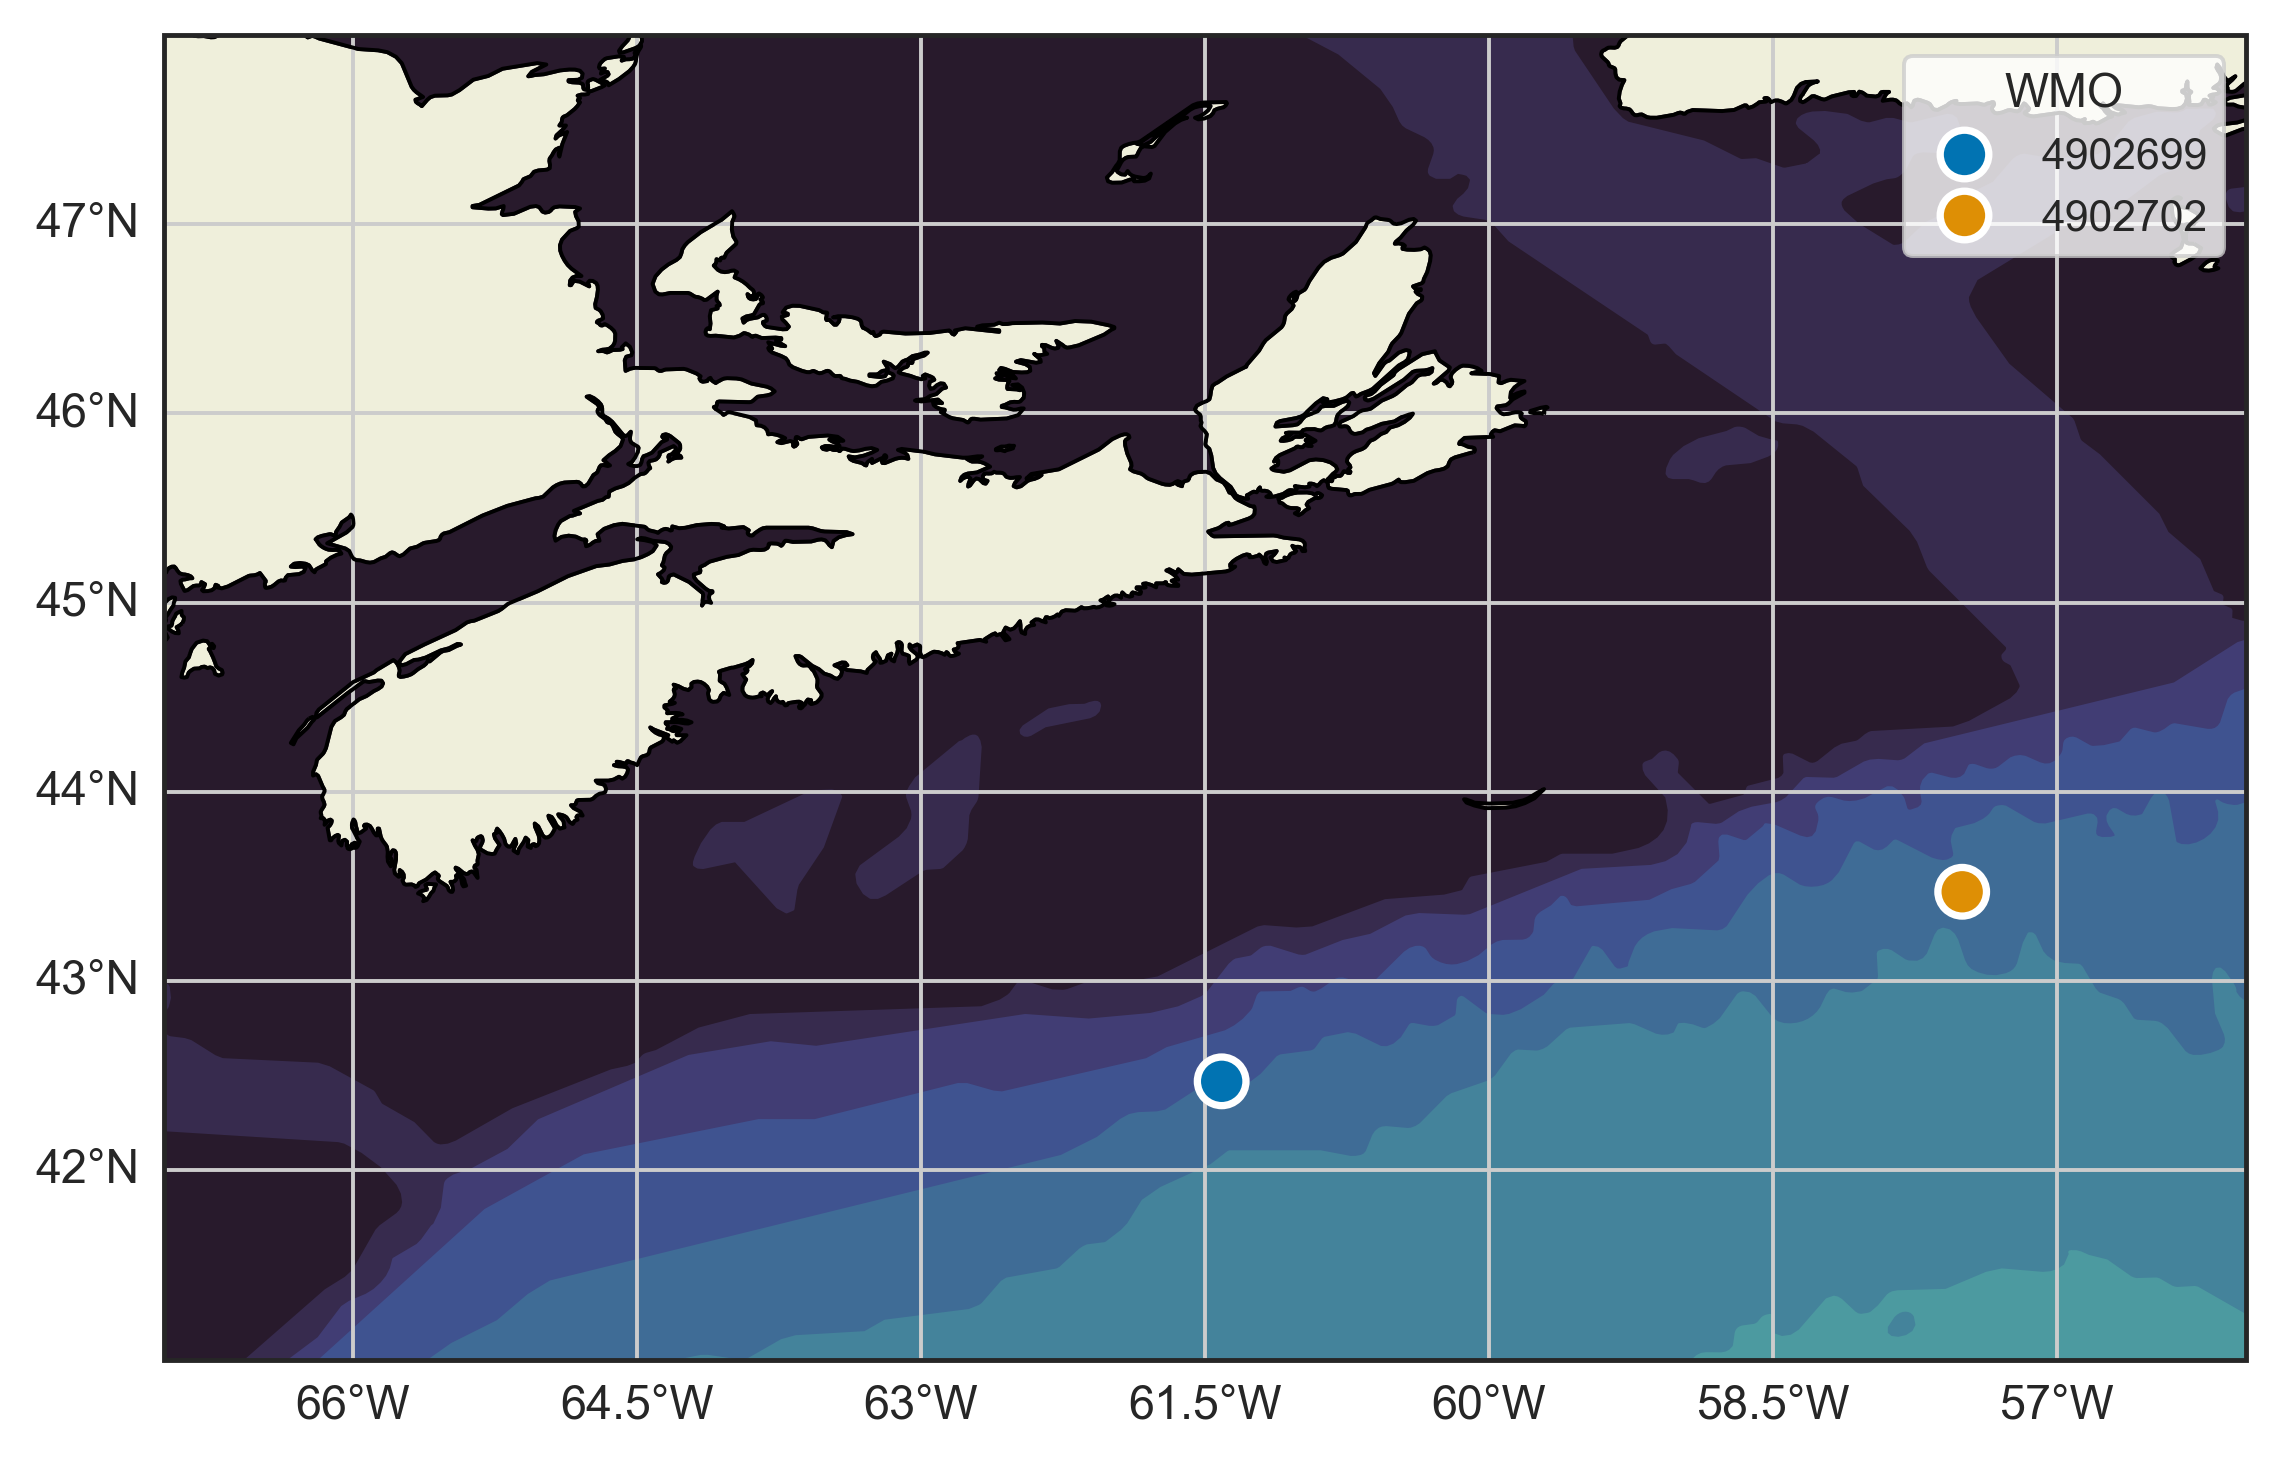
\includegraphics[width=0.9\linewidth]{figs/figure2}}{Figure} 

}

\caption{Location of the Argo float deployments conducted during the 2025 spring AZMP survey (EN728). Solid lines show the Argo profile and square markers on the salinity plots represent bottle salinity measurements collected from the CTD-Rosette casts at stations HL_07 and LL_09, and measured using a salinometer.}\label{fig:figure2}
\end{figure}
\clearpage
\begin{longtable}[t]{>{\raggedright\arraybackslash}p{3em}>{\raggedright\arraybackslash}p{10em}l>{\raggedright\arraybackslash}p{6em}>{\raggedright\arraybackslash}p{3em}>{\raggedright\arraybackslash}p{4em}>{\raggedright\arraybackslash}p{4em}}
\caption{\label{tab:table6}Metadata associated with the deployment of two Argo floats during the 2025 spring AZMP survey (EN728). The WMO and serial numbers (S/N) of each float are provided, along with the time of magnet removal and deployment (UTC), and associated date, event, station, and latitude and longitude (in decimal degrees) of deployment.}\\
\toprule
\begingroup\fontsize{11}{13}\selectfont \textbf{Station}\endgroup & \begingroup\fontsize{11}{13}\selectfont \textbf{Serial No.}\endgroup & \begingroup\fontsize{11}{13}\selectfont \textbf{WMO}\endgroup & \begingroup\fontsize{11}{13}\selectfont \textbf{Deploy. Date}\endgroup & \begingroup\fontsize{11}{13}\selectfont \textbf{Event}\endgroup & \begingroup\fontsize{11}{13}\selectfont \textbf{Lat. (DD)}\endgroup & \begingroup\fontsize{11}{13}\selectfont \textbf{Lon. (DD)}\endgroup\\
\midrule
\begingroup\fontsize{10}{12}\selectfont HL\_07\endgroup & \begingroup\fontsize{10}{12}\selectfont AI2600-24CA008\endgroup & \begingroup\fontsize{10}{12}\selectfont 4902699\endgroup & \begingroup\fontsize{10}{12}\selectfont 2025-04-06\endgroup & \begingroup\fontsize{10}{12}\selectfont 101\endgroup & \begingroup\fontsize{10}{12}\selectfont 42.4705\endgroup & \begingroup\fontsize{10}{12}\selectfont -61.4103\endgroup\\
\begingroup\fontsize{10}{12}\selectfont LL\_09\endgroup & \begingroup\fontsize{10}{12}\selectfont AI2600-24CA011\endgroup & \begingroup\fontsize{10}{12}\selectfont 4902702\endgroup & \begingroup\fontsize{10}{12}\selectfont 2025-04-11\endgroup & \begingroup\fontsize{10}{12}\selectfont 154\endgroup & \begingroup\fontsize{10}{12}\selectfont 43.4719\endgroup & \begingroup\fontsize{10}{12}\selectfont -57.4984\endgroup\\
\bottomrule
\end{longtable}
\begin{figure}[htb]

{\centering \pdftooltip{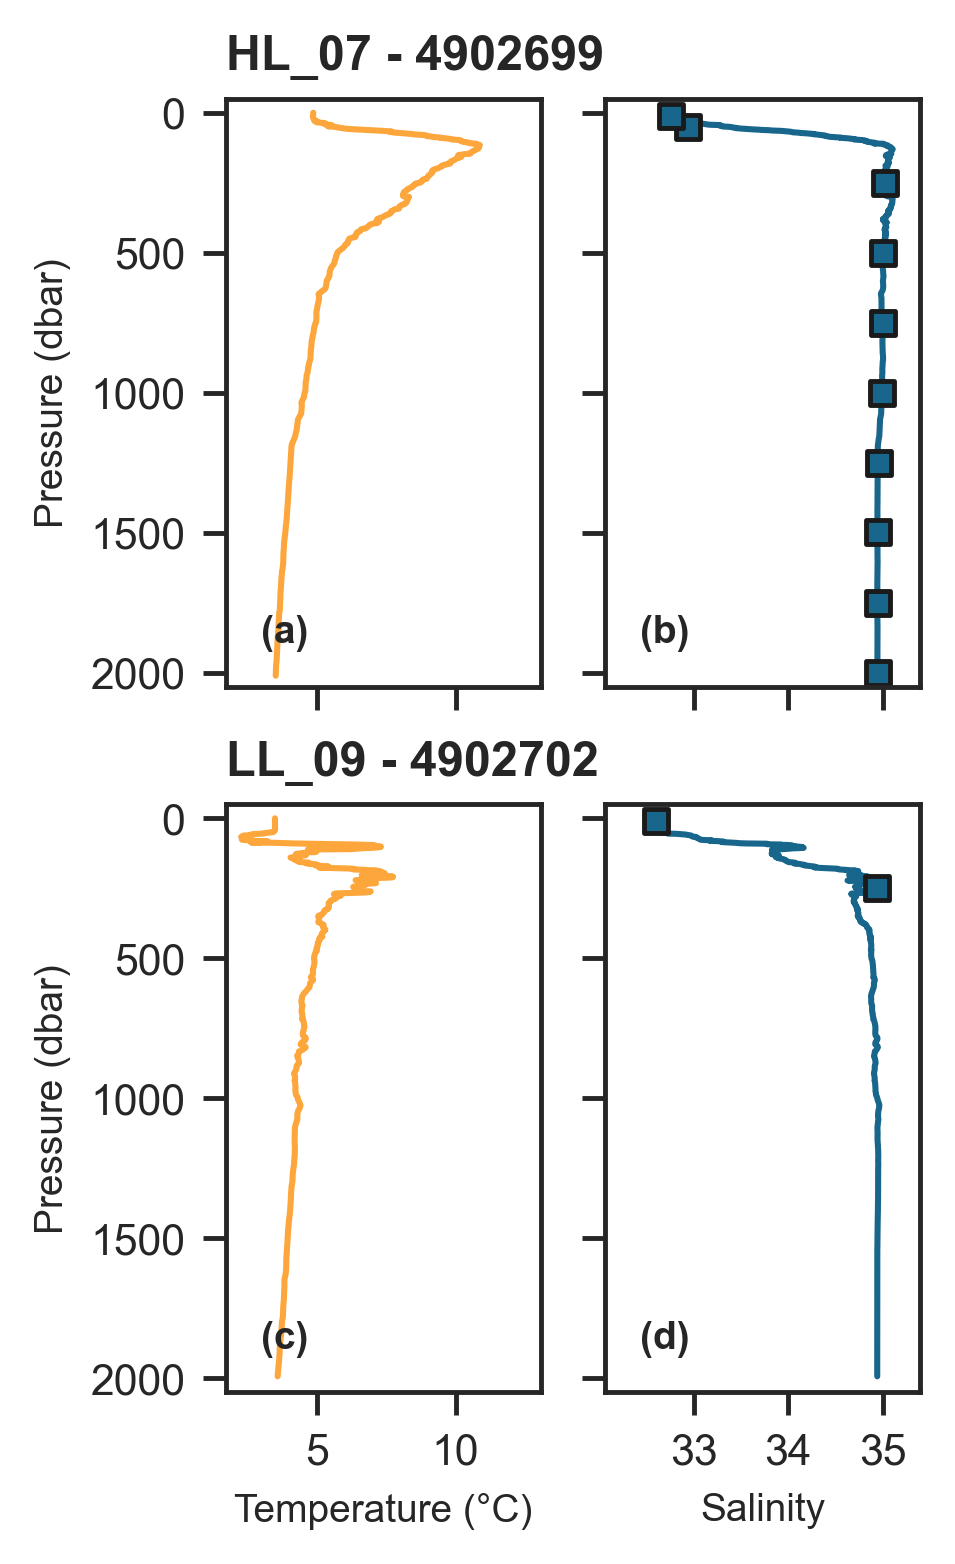
\includegraphics[width=3.18in]{figs/figure3}}{Figure} 

}

\caption{Initial profile for Argo floats 4902699 and 4902702 deployed at stations HL_07 and LL_09 respectively, during the 2025 spring AZMP mission (EN728).}\label{fig:figure3}
\end{figure}
\clearpage

\subsection{Flow-Through Systems}\label{flow}

\subsubsection{TSG system and associated sensors}\label{tsg-system-and-associated-sensors}

Continuous surface measurements of temperature, conductivity, salinity, dissolved oxygen, pH, chlorophyll \emph{a}, and coloured dissolved organic matter (CDOM) were collected via a portable flow-through system operated and maintained by BIO's Ocean Engineering and Technology Section (OETS) installed in the Wet Laboratory on the RV \emph{Endeavor}. This system consisted of three tanks which hold a SBE 21 SeaCAT Thermosalinograph (TSG; tank 1), a SBE 18 pH sensor, Aanderaa optode dissolved oxygen sensor, and Seapoint UV CDOM and chlorophyll fluorometers sensors (tank 2), and a General Oceanics pCO\(_2\) sensor (tank 3). A debubbler system was installed to reduce air flow through the tanks. This flow-through system was connected to the vessel's uncontaminated science seawater dispersed throughout the vessel via an impeller pump. The seawater intake for this pump was located near the bow of the vessel at 5 m below the sea surface. Temperature at the intake was recorded using an SBE 38 located approximately 12'' from the intake.

On April 6, it was discovered that the impeller pump had been experiencing sporadic shutdowns throughout the mission, which became more persistent. A decision was then made to switch the water source to a second science seawater system on the \emph{Endeavor} that was modulated via a diaphragm pump. This conversion occurred on April 14. The intake temperature for the impeller pump continued to be fed into the flow-through system. While the intake depth for the diaphragm pump was also 5 m depth, diaphragm pumps are known to produce less shear stress on phytoplankton cells compared to impeller pumps (\citeproc{ref-Cetinic_2016}{Cetinić et al. 2016}), potentially resulting in higher-quality optical measurements. However, the diaphragm pump appeared to create pulses in the flow and pressure of water through the flow-through system, potentially impacting other sensor outputs (e.g., dissolved oxygen). Future end users of the chlorophyll data collected on this mission should be aware of compatibility issues of the data collected with the impeller pump system versus the diaphragm pump system.

At approximately 08:12 UTC on Monday April 14, the impeller pump power source failed. This resulted in the loss of data from the intake temperature sensor to the system. Shortly thereafter, a decision was made to connect the temperature sensor located in the ship's transducer well, also located 5 m from the hull of the vessel, to the flow-through system via serial feed. This was used as the intake temperature source for the remainder of the EN728 mission.

The RV \emph{Endeavor} also has a shipboard flow-through system installed in the Wet Laboratory on board, which was active during the mission. This system is described further in the \hyperref[shipboard-systems]{Shipboard Science Systems} section below.

\paragraph{Daily underway system sampling}\label{daily-underway-system-sampling}

Daily sampling of dissolved oxygen, chlorophyll, salinity, CDOM, and TIC/TA samples were collected from the outflow of the BIO flow-through system throughout the mission (see Table~\ref{tab:table7}). Samples were collected daily at approximately noon, starting on March 30 and ending on April 17. Daily samples were assigned a unique sample ID for each day, which was recorded in the ELOG metadata logger. The sample ID range for daily underway samples collected during the mission was 514003 to 514021.

\clearpage

\pagestyle{empty}
\begin{landscape}
\begin{longtable}[t]{l>{\raggedright\arraybackslash}p{4em}>{\raggedright\arraybackslash}p{4em}>{\raggedright\arraybackslash}p{4em}ll>{\raggedright\arraybackslash}p{4em}>{\raggedright\arraybackslash}p{4em}>{\raggedright\arraybackslash}p{4em}>{\raggedright\arraybackslash}p{2em}>{\raggedright\arraybackslash}p{1.5em}>{\raggedright\arraybackslash}p{1.5em}lll}
\caption{\label{tab:table7}Metadata associated with the collection of water samples from the underway system during the 2025 spring AZMP mission (EN728). Date, time (UTC), latitude and longitude (in decimal degrees) of the ship's position were recorded in ELOG at the time of sample entry, while temperature (°C), salinity, and pH were recorded from the thermosalinograph. 'X' and 'XX' indicate single and duplicate sampling, respectively. CM = coloured dissolved organic matter.}\\
\toprule
\multicolumn{1}{c}{\bgroup\fontsize{12}{14}\selectfont \textbf{ }\egroup{}} & \multicolumn{1}{c}{\bgroup\fontsize{12}{14}\selectfont \textbf{ }\egroup{}} & \multicolumn{1}{c}{\bgroup\fontsize{12}{14}\selectfont \textbf{ }\egroup{}} & \multicolumn{1}{c}{\bgroup\fontsize{12}{14}\selectfont \textbf{ }\egroup{}} & \multicolumn{1}{c}{\bgroup\fontsize{12}{14}\selectfont \textbf{ }\egroup{}} & \multicolumn{1}{c}{\bgroup\fontsize{12}{14}\selectfont \textbf{ }\egroup{}} & \multicolumn{1}{c}{\bgroup\fontsize{12}{14}\selectfont \textbf{ }\egroup{}} & \multicolumn{1}{c}{\bgroup\fontsize{12}{14}\selectfont \textbf{ }\egroup{}} & \multicolumn{1}{c}{\bgroup\fontsize{12}{14}\selectfont \textbf{ }\egroup{}} & \multicolumn{6}{c}{\bgroup\fontsize{12}{14}\selectfont \textbf{Bottle Samples}\egroup{}} \\
\cmidrule(l{3pt}r{3pt}){10-15}
\begingroup\fontsize{11}{13}\selectfont \textbf{Date}\endgroup & \begingroup\fontsize{11}{13}\selectfont \textbf{Time (UTC)}\endgroup & \begingroup\fontsize{11}{13}\selectfont \textbf{Lat. (DD)}\endgroup & \begingroup\fontsize{11}{13}\selectfont \textbf{Lon. (DD)}\endgroup & \begingroup\fontsize{11}{13}\selectfont \textbf{Temp}\endgroup & \begingroup\fontsize{11}{13}\selectfont \textbf{Sal}\endgroup & \begingroup\fontsize{11}{13}\selectfont \textbf{Sample ID}\endgroup & \begingroup\fontsize{11}{13}\selectfont \textbf{TSG Flow Rate (L/min)}\endgroup & \begingroup\fontsize{11}{13}\selectfont \textbf{pCO2 Flow Rate (L/min)}\endgroup & \begingroup\fontsize{11}{13}\selectfont \textbf{pCO2}\endgroup & \begingroup\fontsize{11}{13}\selectfont \textbf{TIC/ TA}\endgroup & \begingroup\fontsize{11}{13}\selectfont \textbf{Chl}\endgroup & \begingroup\fontsize{11}{13}\selectfont \textbf{Salts}\endgroup & \begingroup\fontsize{11}{13}\selectfont \textbf{O2}\endgroup & \begingroup\fontsize{11}{13}\selectfont \textbf{CM}\endgroup\\
\midrule
2025-03-30 & 16:29:00 & 42.5351 & -65.4862 & 2.75 & 31.23 & 514003 & 10.1 & 1.86 & X & X & XX & X & X & X\\
2025-03-31 & 15:22:00 & 43.2516 & -66.2608 & 4.47 & 32.05 & 514004 & 15.0 & 2.00 & X & X & XX & X & X & X\\
2025-04-01 & 15:58:00 & 43.3825 & -68.8018 & 4.88 & 32.58 & 514005 & 14.8 & 1.91 & X & X & XX & X & X & X\\
2025-04-02 & 15:16:00 & 42.8400 & -68.8990 & 5.54 & 32.72 & 514006 & 15.2 & 1.88 & X & X & XX & X & X & X\\
2025-04-03 & 15:52:00 & 42.0631 & -66.0843 & 4.95 & 32.15 & 514007 & 15.2 & 1.82 & X & X & XX & X & X & X\\
2025-04-04 & 15:23:00 & 43.5395 & -64.4049 & 2.79 & 31.22 & 514008 & 15.2 & 2.05 & X & X & XX & X & X & X\\
2025-04-05 & 16:32:00 & 43.1467 & -62.0617 & 4.45 & 32.37 & 514009 & 14.3 & 2.06 & X & X & XX & X & X & X\\
2025-04-06 & 15:35:00 & 42.7105 & -60.9526 & 6.06 & 32.40 & 514010 & 14.6 & 1.99 & X & X & XX & X & X & X\\
2025-04-07 & 15:38:00 & 44.1566 & -59.1874 & 3.35 & 32.05 & 514011 & 14.6 & 2.07 & X & X & XX & X & X & X\\
2025-04-08 & 16:22:00 & 44.1328 & -59.2316 & 2.96 & 32.13 & 514012 & 13.0 & 1.84 & X & X & XX & X & X & X\\
2025-04-09 & 15:25:00 & 44.6158 & -57.7419 & 2.44 & 32.13 & 514013 & 12.7 & 1.97 & X & X & XX & X & X & X\\
2025-04-10 & 18:41:00 & 45.0008 & -56.0294 & 1.75 & 32.51 & 514014 & 10.1 & 0.93 & X & X & XX & X & X & X\\
2025-04-11 & 18:14:00 & 43.9202 & -57.9609 & 4.00 & 32.60 & 514015 & 16.1 & 2.35 & X & X & XX & X & X & X\\
2025-04-12 & 17:19:00 & 45.9048 & -59.6683 & 1.45 & 30.41 & 514016 & 15.2 & 2.15 & X & X & XX & X & X & X\\
2025-04-13 & 15:37:00 & 47.4254 & -59.2054 & 1.03 & 30.96 & 514017 & 15.4 & 2.27 & X & X & XX & X & X & X\\
2025-04-14 & 15:37:00 & 45.3385 & -59.6573 & 2.35 & 31.08 & 514018 & 15.8 & 2.31 & X & X & XX & X & X & X\\
2025-04-15 & 16:49:00 & 43.7269 & -61.4914 & 4.59 & 32.23 & 514019 & 14.7 & 1.92 & X & X & XX & X & X & X\\
2025-04-16 & 19:09:00 & 41.8939 & -60.9807 & 5.64 & 31.76 & 519020 & 14.5 & 1.77 & X & X & XX & X & X & X\\
2025-04-17 & 15:15:00 & 43.4533 & -62.3011 & 4.49 & 31.91 & 519021 & 15.9 & 1.96 & X & X & XX & X & X & X\\
\bottomrule
\end{longtable}
\end{landscape}
\clearpage

\pagestyle{plain}

\paragraph{Data management and sensor validation}\label{data-management-and-sensor-validation}

The Advanced Serial Data Logger software installed on the BIO flow-through computer system records the TSG, flow rate, NMEA data, and pCO\(_2\) RS-232 serial data directly into text (.csv) files produced daily. The frequency of measurements within each file type varies, with NMEA recordings occurring every second, TSG measurements every 5 seconds, and flow data approximately every second. A script was developed using R statistical software to collate the TSG and flow rate data with the corresponding positional data in the NMEA file. Measurements were interpolated in hourly bins and plotted to visualize spatial patterns and help validate the sensor outputs (see Figures~\ref{fig:figure4} and~\ref{fig:figure5} below). The optode calphase output is converted to dissolved oxygen concentration in ml/L whilst correcting for salinity (in the tank) using R.

As oxygen, chlorophyll and salinity samples taken collected from the outflow from the flow-through system are processed on board, the resulting bottle sample values were plotted against the corresponding flow-through sensor data throughout the mission (see Figure~\ref{fig:figure6}) to validate the sensor outputs. Dissolved oxygen concentration measured by the optode sensor was consistently higher than the corresponding bottle measurements throughout the mission (mean difference = 0.9872 ± 0.1296 ml/L). In contrast, there was relatively good congruence between sensor salinity values and bottle salinity measurements evaluated across the mission (mean difference = -0.0321 ± 0.1551). An exception occurred on April 6, when the daily bottle salinity measurement (32.8583) was nearly 1 unit of measure higher than its corresponding sensor salinity measurement (32.2082). The fluorometer chlorophyll \emph{a} values were consistently lower than their corresponding Turner chlorophyll \emph{a} replicates throughout the mission. This pattern was particularly pronounced during periods of higher daily chlorophyll \emph{a} measurements, and is consistent with the observation of lower CTD fluorometer values relative to the Turner sample values at the depth of the chlorophyll \emph{a} maximum.

\subsubsection{Imaging Flow Cytobot}\label{imaging-flow-cytobot}

As part of a collaborative agreement with the Woods Hole Center for Oceans and Human Health (WHCOHH), an Imaging FlowCytobot (IFCB) was installed in the Special Purpose Laboratory prior to the vessel's departure from Narragansett. This system is designed to draw small seawater samples from its environment (or in this case, from the ship's science seawater system) every 23 minutes using a syringe pump, which then pushes a thin stream of the sampled water across a microscope objective. Cells and other particles are detected by an in-line laser immediately upstream of the objective. Detections trigger a precisely-timed flash lamp that illuminates the cell/particle just as it passes in front of the microscope objective. Images of cells are captured by a charged-coupled device (CCD) camera and stored in data files that are associated with each seawater sample. Raw data includes gray-scale images of each particle and associated measurements of laser scatter and fluorescence. This system requires a minimum flow rate of 2 L/min, and the total volume sampled is 25 mL per hour.

The collected images are accessible via an in-house IFCB \link{https://habon-ifcb.whoi.edu/hablab_en728}{dashboard}. Due to connectivity issues, IFCB data was not collected while the vessel was sampling the Laurentian Channel Mouth line, but is otherwise available for the entire mission track.

\clearpage
\begin{landscape}


\begin{figure}[H]

{\centering \pdftooltip{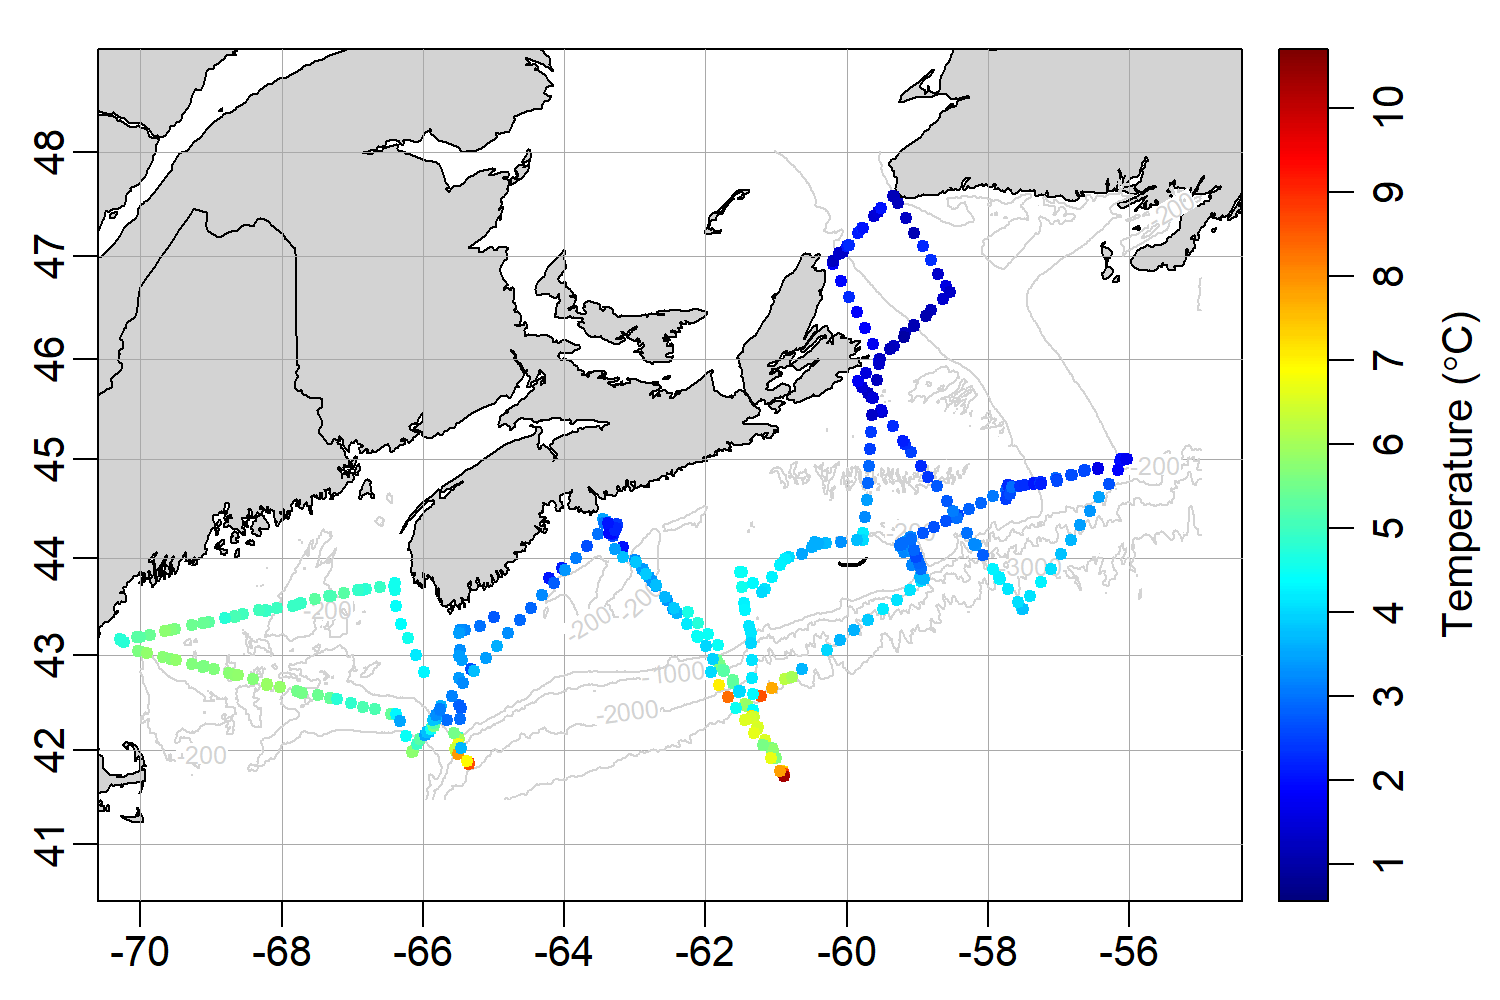
\includegraphics[width=0.47\linewidth,height=0.41\textheight]{figs/figure4a}}{Figure} \pdftooltip{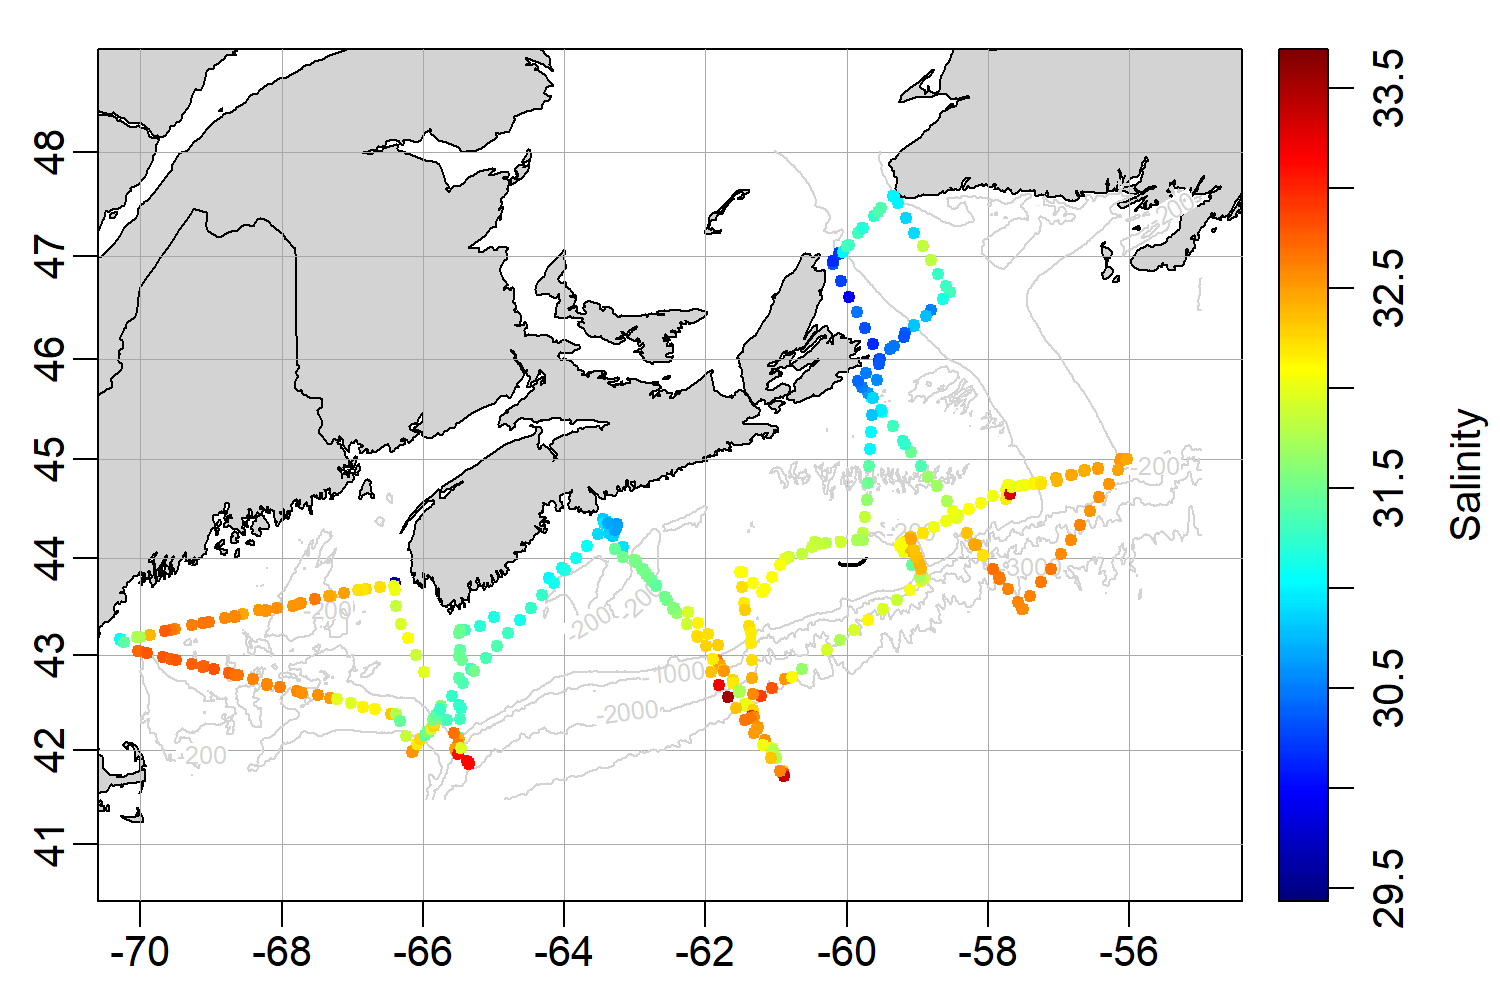
\includegraphics[width=0.47\linewidth,height=0.41\textheight]{figs/figure4b}}{Figure} \pdftooltip{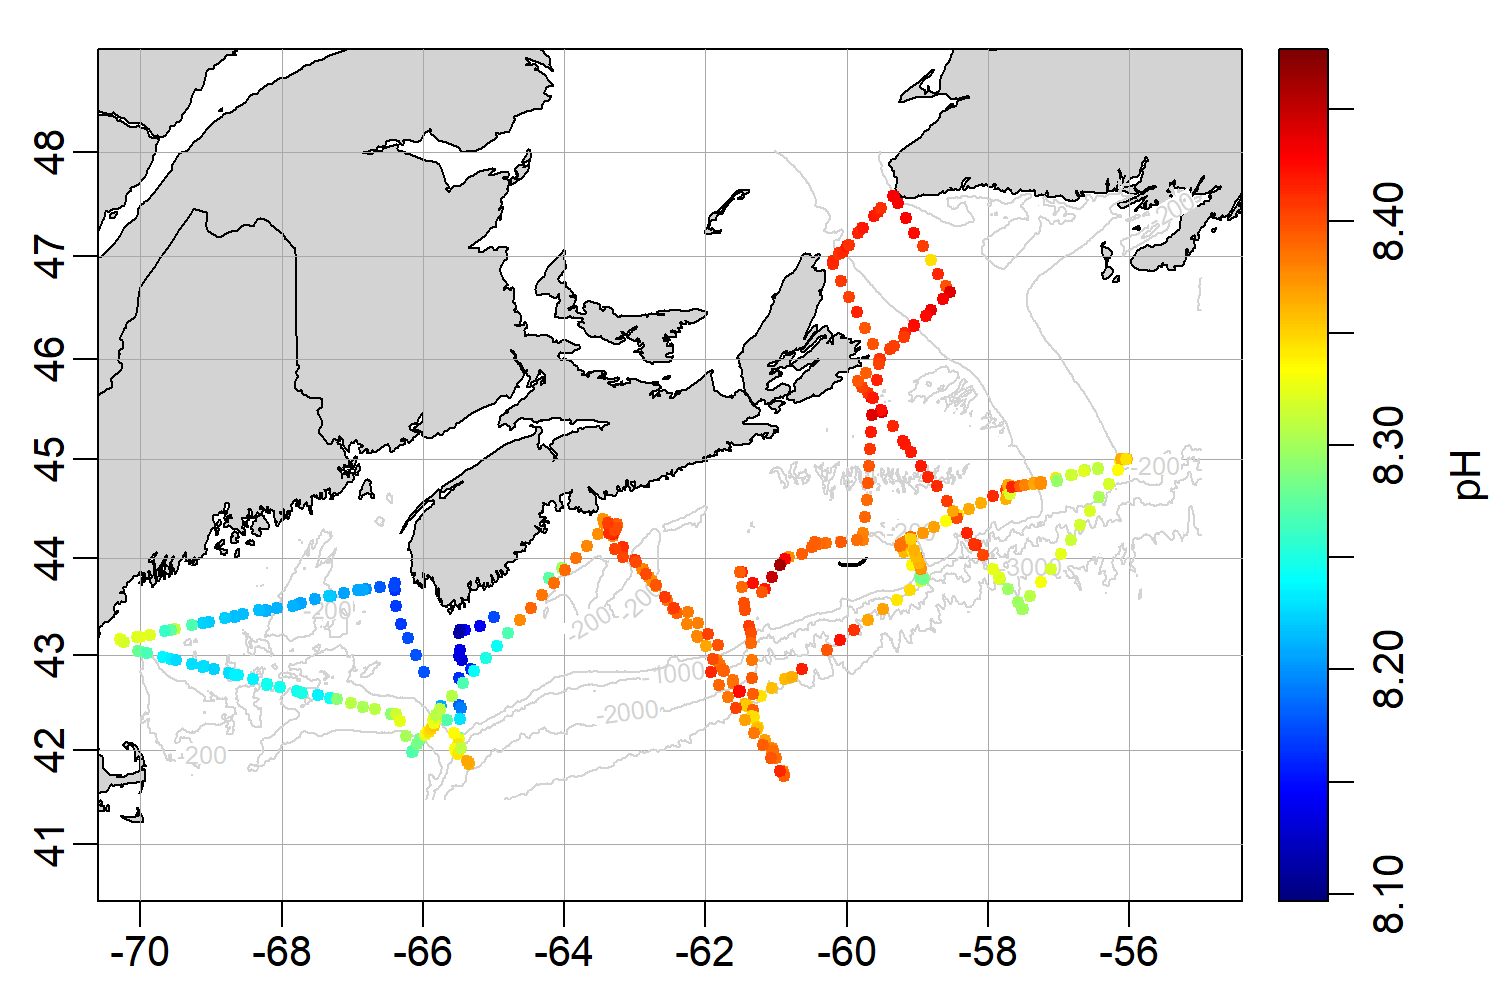
\includegraphics[width=0.47\linewidth,height=0.41\textheight]{figs/figure4c}}{Figure} \pdftooltip{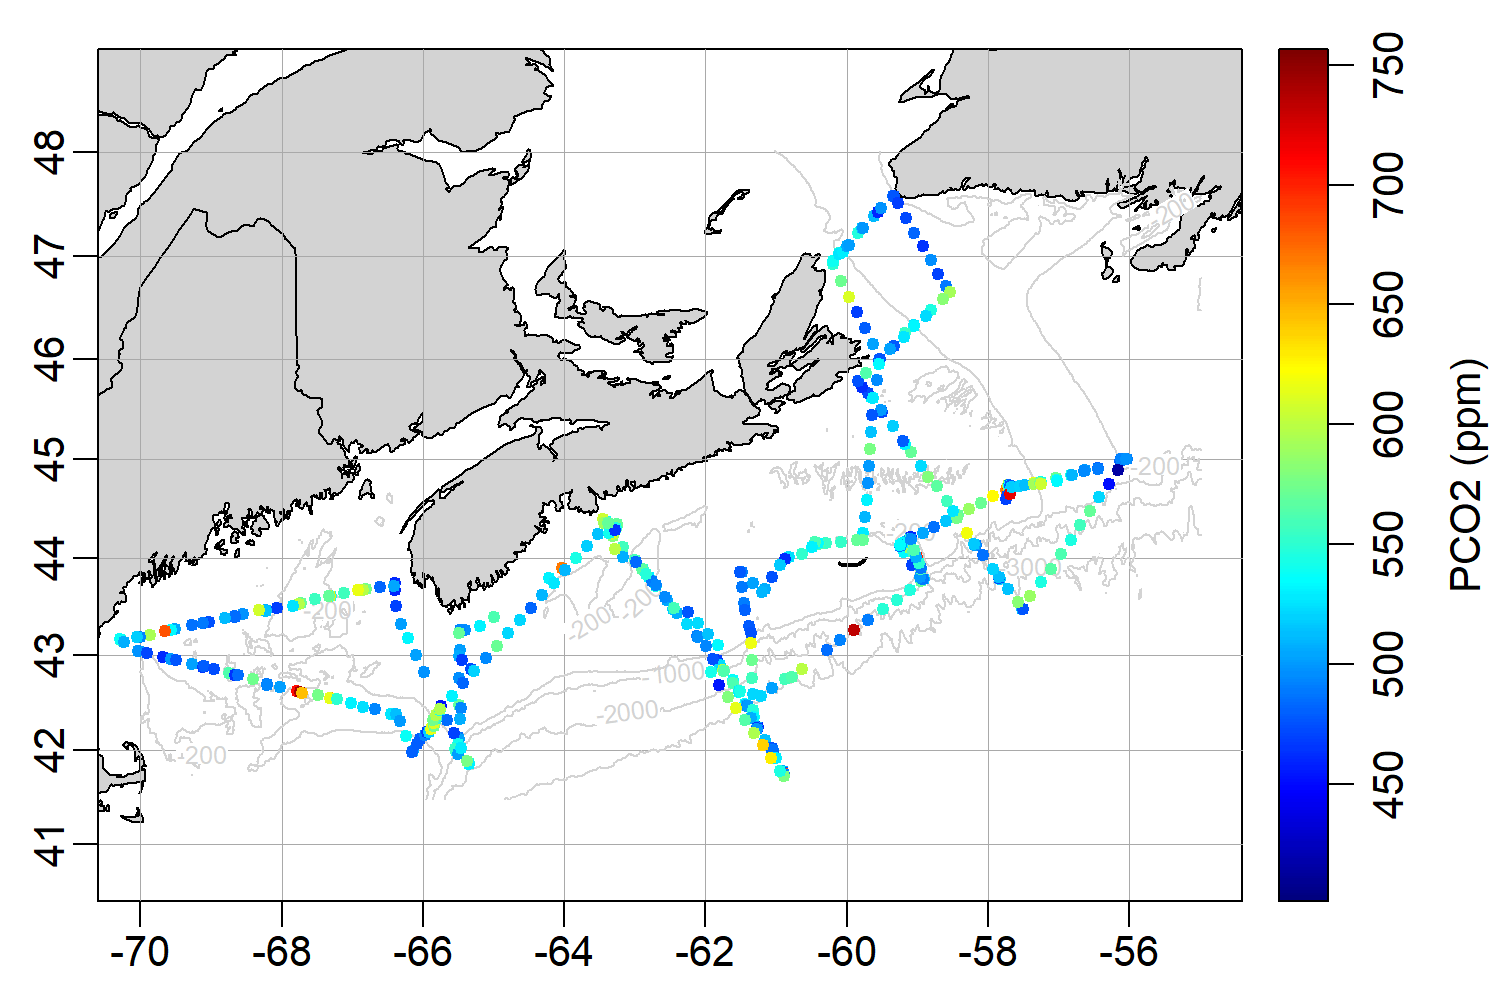
\includegraphics[width=0.47\linewidth,height=0.41\textheight]{figs/figure4d}}{Figure} 

}

\caption{Surface temperature ($^\circ$C; top left), salinity (top right), pH (lower left), and the partial pressure of carbon dioxide (pCO$_{2}$; lower right) measured along the cruise track during the 2025 spring AZMP mission (EN728). Data are measured at variable intervals and presented as hourly interpolations.  }\label{fig:figure4}
\end{figure}
\end{landscape}
\pagestyle{plain}


\begin{figure}[H]

{\centering \pdftooltip{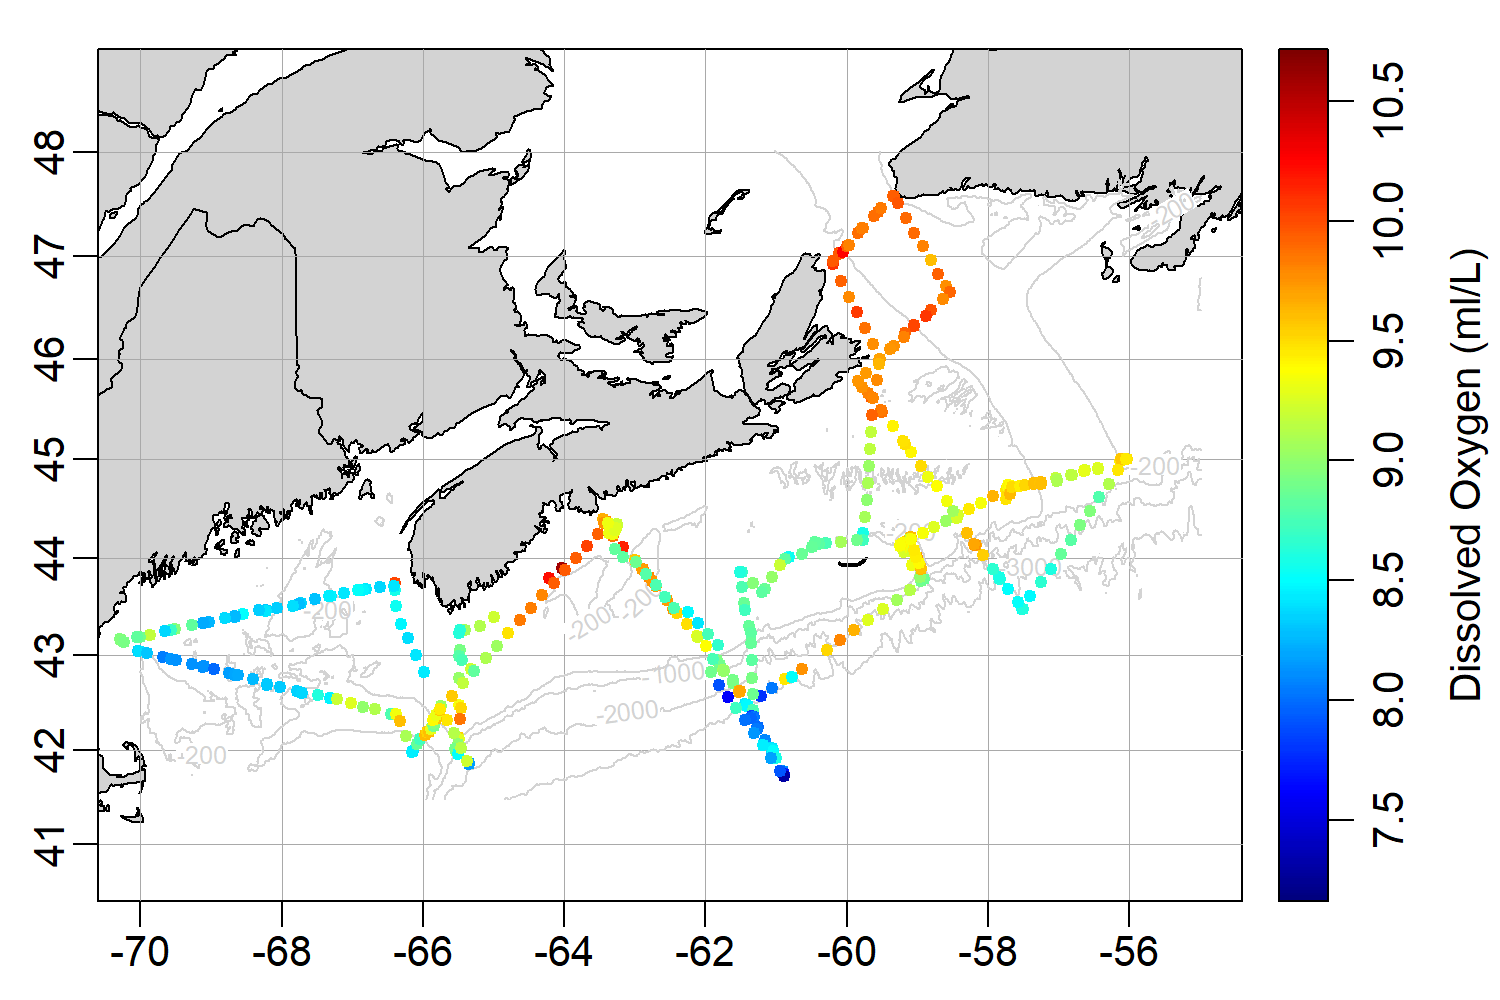
\includegraphics[width=0.7\linewidth,height=0.29\textheight,angle=360]{figs/figure5a}}{Figure} \pdftooltip{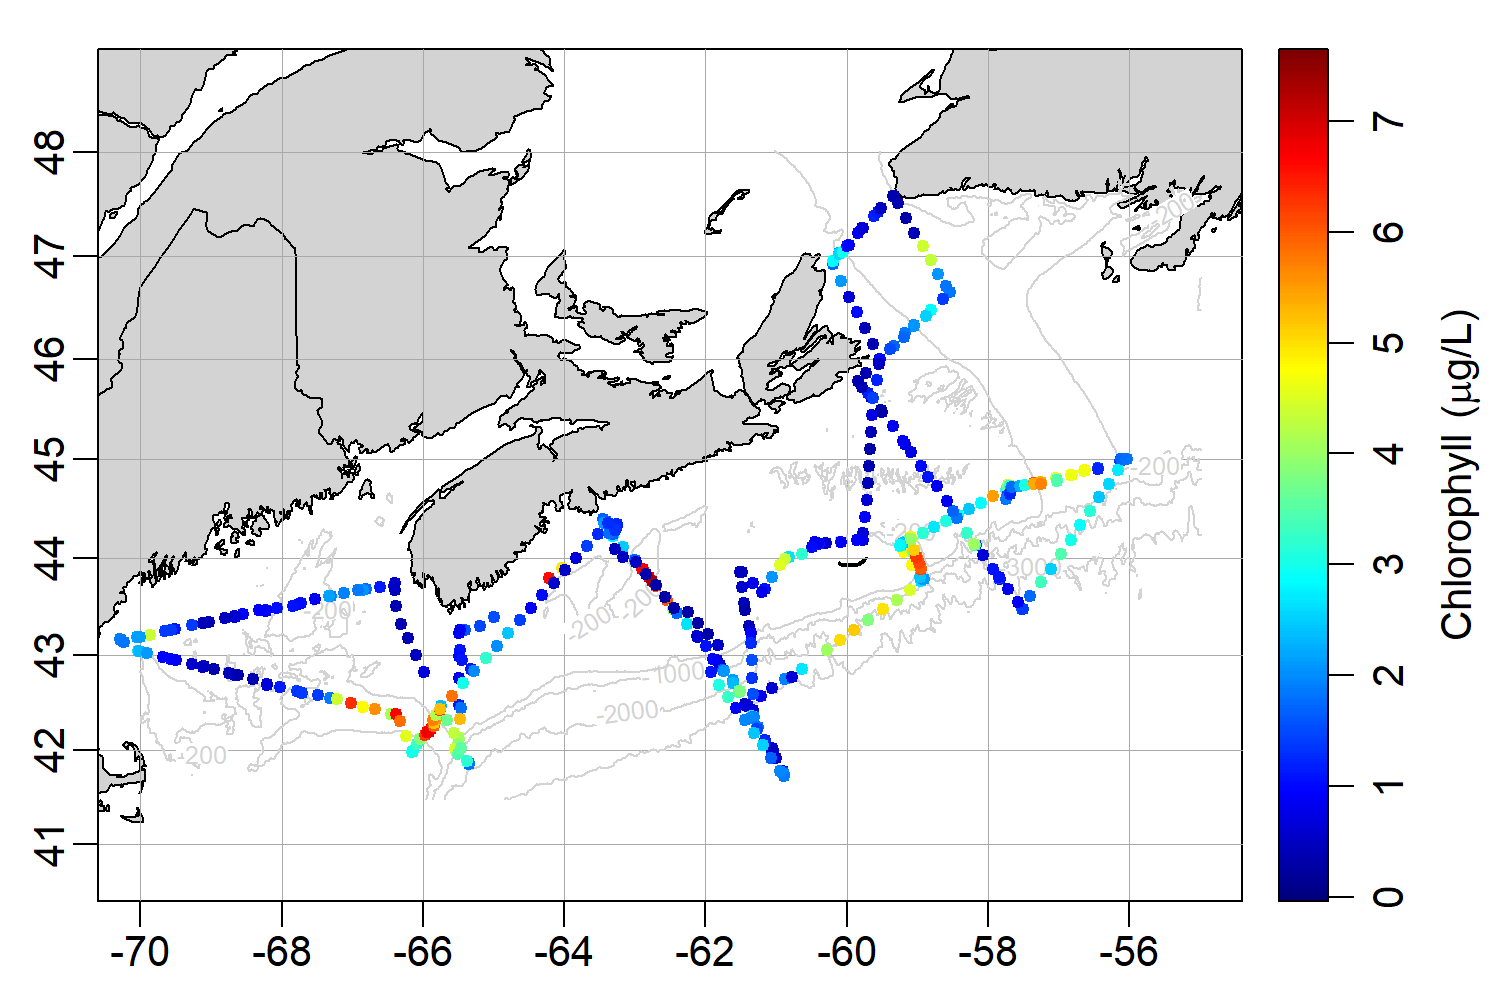
\includegraphics[width=0.7\linewidth,height=0.29\textheight,angle=360]{figs/figure5b}}{Figure} \pdftooltip{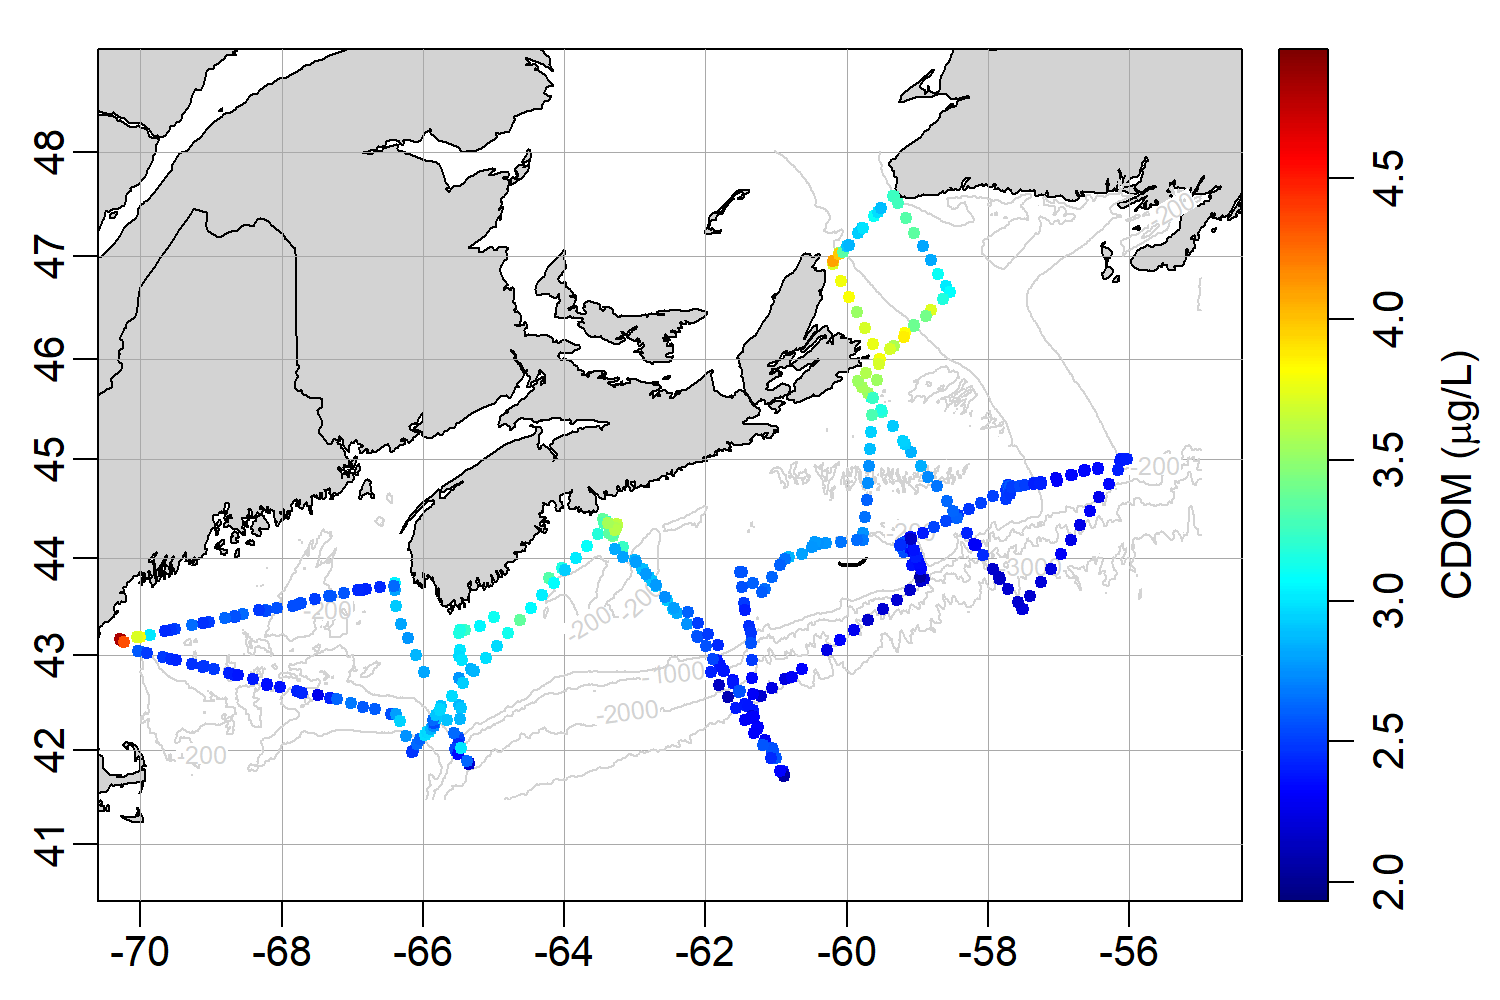
\includegraphics[width=0.7\linewidth,height=0.29\textheight,angle=360]{figs/figure5c}}{Figure} 

}

\caption{Dissolved oxygen concentration (ml/L; top), chlorophyll fluorescence (\(\mu g\)/L; middle), and CDOM (\(\mu g\)/L; bottom) measured along the cruise track during the 2025 spring AZMP mission (EN728). Data are measured at variable intervals and presented as hourly interpolations.}\label{fig:figure5}
\end{figure}
\clearpage


\begin{figure}[htb]

{\centering \pdftooltip{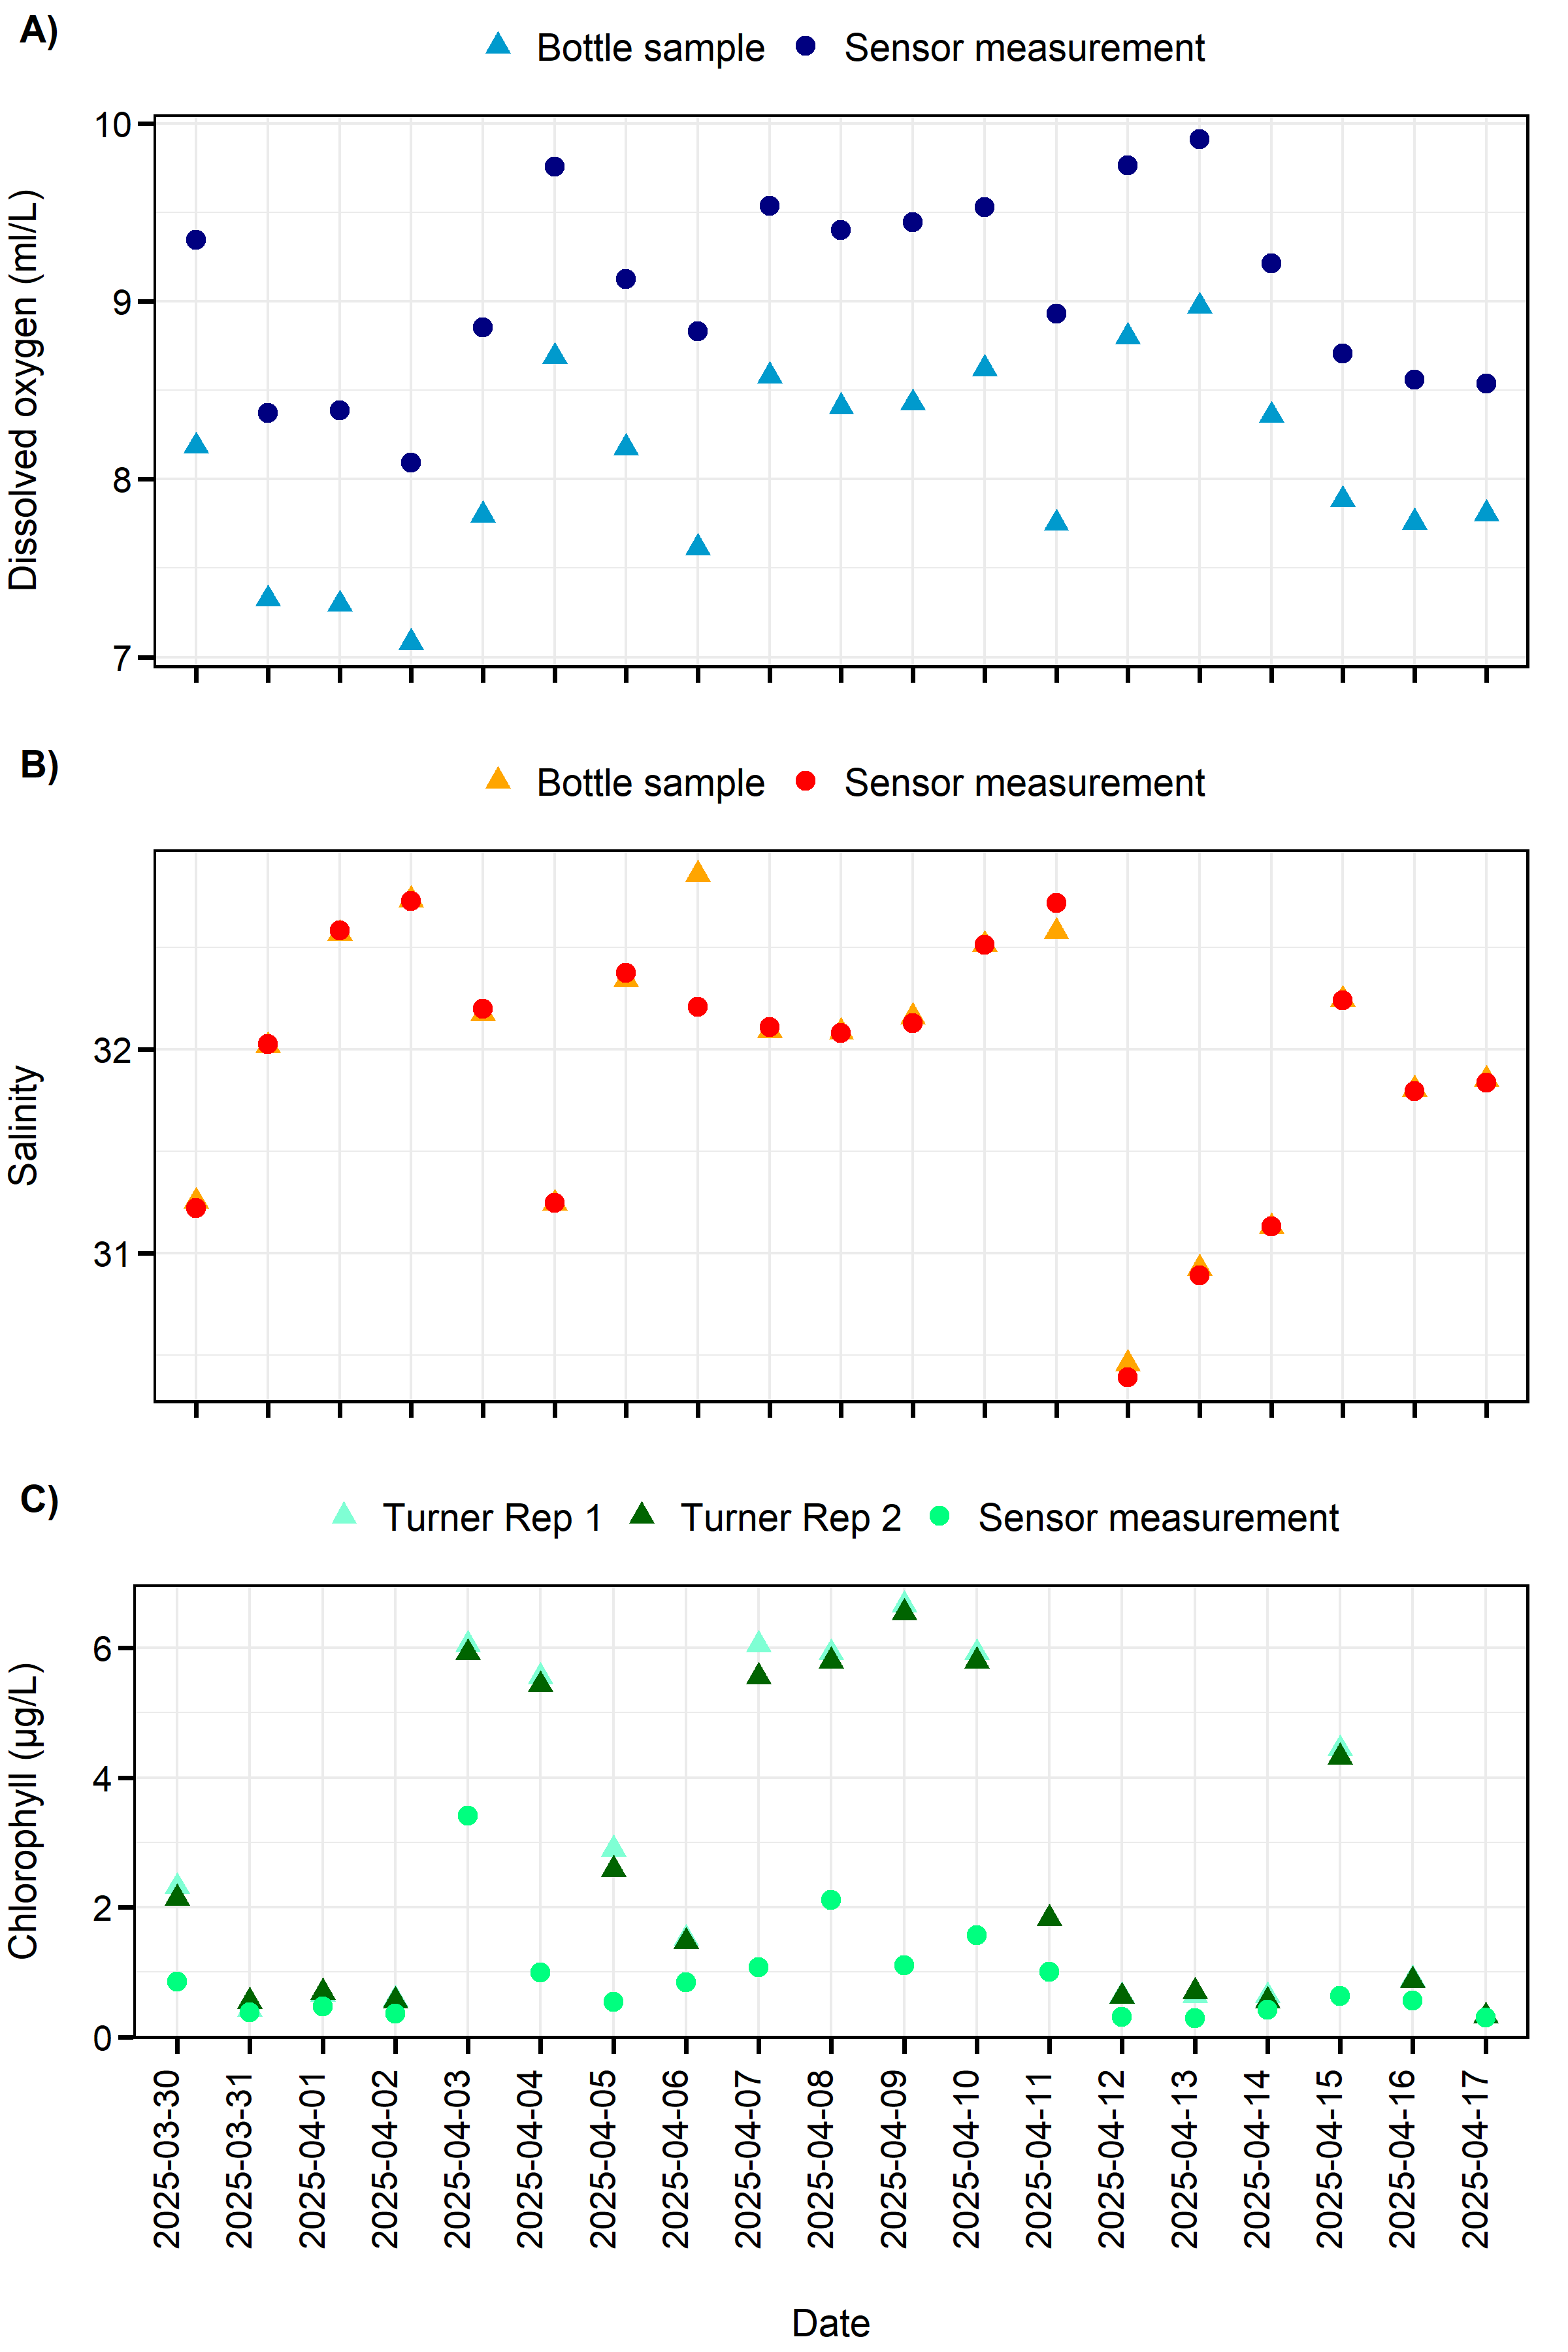
\includegraphics[width=0.85\linewidth]{figs/figure6}}{Figure} 

}

\caption{Comparison between bottle samples and sensor measurements of A) dissolved oxygen, B) salinity and C) chlorophyll collected using BIO's portable flow-through system installed on the RV \emph{Endeavor} during the 2025 spring AZMP survey.}\label{fig:figure6}
\end{figure}
\clearpage

\subsection{Mooring Operations}\label{mooring-operations}

Deployment of a single passive acoustic monitoring (PAM) mooring was conducted in Roseway Basin on the EN728 mission. This mooring consisted of a large Stablemoor capsule floatation with an inserted JASCO Autonomous Multichannel Acoustic Recorder, battery pack, hydrophone, beacon, and SBE 37 microCAT connected to two BUB buoyancy packages via a kevlar rope, and dual Teledyne Benthos acoustic releases connected to a double train wheel anchor weighing 1240 lbs. The total length of the mooring assembly was 29 m in length with an in-air weight of 1678 lbs (excluding the anchor). This mooring was deployed in the Roseway Basin North Atlantic Right Whale critical habitat zone at the request of DFO Research Scientist Angelia Vanderlaan, lead of DFO's North Atlantic Right Whale Research Unit, Maritimes Region, after it unexpectedly resurfaced in December 2024 due to a failed release. The mooring was deployed using the vessel's A-frame and a portable Tension Strain Equipment (TSE) mooring spooler provided by URI. The mooring will remain until its recovery in fall 2025.

An array of 15 acoustic receiver moorings situated at the head of the Gully MPA (see Figure~\ref{fig:figure7}) was planned for recovery during the EN728 mission as part of a joint project between DFO and the Ocean Tracking Network (OTN). These moorings were outfitted with acoustic releases and yellow flotation collars outfitted with Vemco VR4 receivers that sit several metres above the seabed that are designed to record nearby tagged species. The goal of this project was to understand how a hot spot of juvenile halibut northwest of the MPA utilize the area, providing key insights into their behavior and movement patterns.

A recovery procedure was outlined between the lead mooring technician on the mission, Adam Hartling, the Captain and bosun, which involved positioning the vessel approximately 150 m away from the mooring coordinates and establishing communications with the mooring using a Vemco VR100 deck unit and transducer deployed to 5-6 m below the sea surface. Once the mooring was released, the vessel positioned itself so that the mooring flotation was accessible from the starboard deck. Once the flotation was alongside and close enough to reach, a long gaff was used to hook a loop in the rope leading from the flotation to the release. A snap hook attached to a rope connected to the ship's knuckleboom crane was then used to secure the mooring and lift it out of the water and onto the starboard deck. Once the mooring and release were on board, they were cleaned of any biofouling material and stowed for the remainder of the mission.

Of the 15 moorings comprising the array, only 12 could be recovered. Most moorings (see Table~\ref{tab:table3}) were recovered on Monday April 7, with the exception of the moorings at stations GUL02, GUL03, GUL05, and GUL12. Of these 4, communications could not be established with the moorings at GUL05 and GUL12. At stations GUL02 and GUL03, communications were established, but neither mooring surfaced after release. A health status evaluation indicated that the depth of both moorings did not change after release. The tilt of each mooring release was high (56 to 79\(^\circ\)) suggesting the releases were not vertical in the water column. The moorings that could not be recovered on April 7 were revisited on Tuesday April 8 to attempt recovery for a second time. Upon arrival at station GUL12, communications were established with the mooring almost immediately, and it was released and recovered successfully. However, communications could not be established with the mooring release at GUL05, and this mooring could not be recovered. The moorings at stations GUL02 and GUL03 were revisited and communications re-established, but their status remained unchanged. Release was re-attempted for both moorings but was not successful.

\clearpage
\begin{figure}[htb]

{\centering 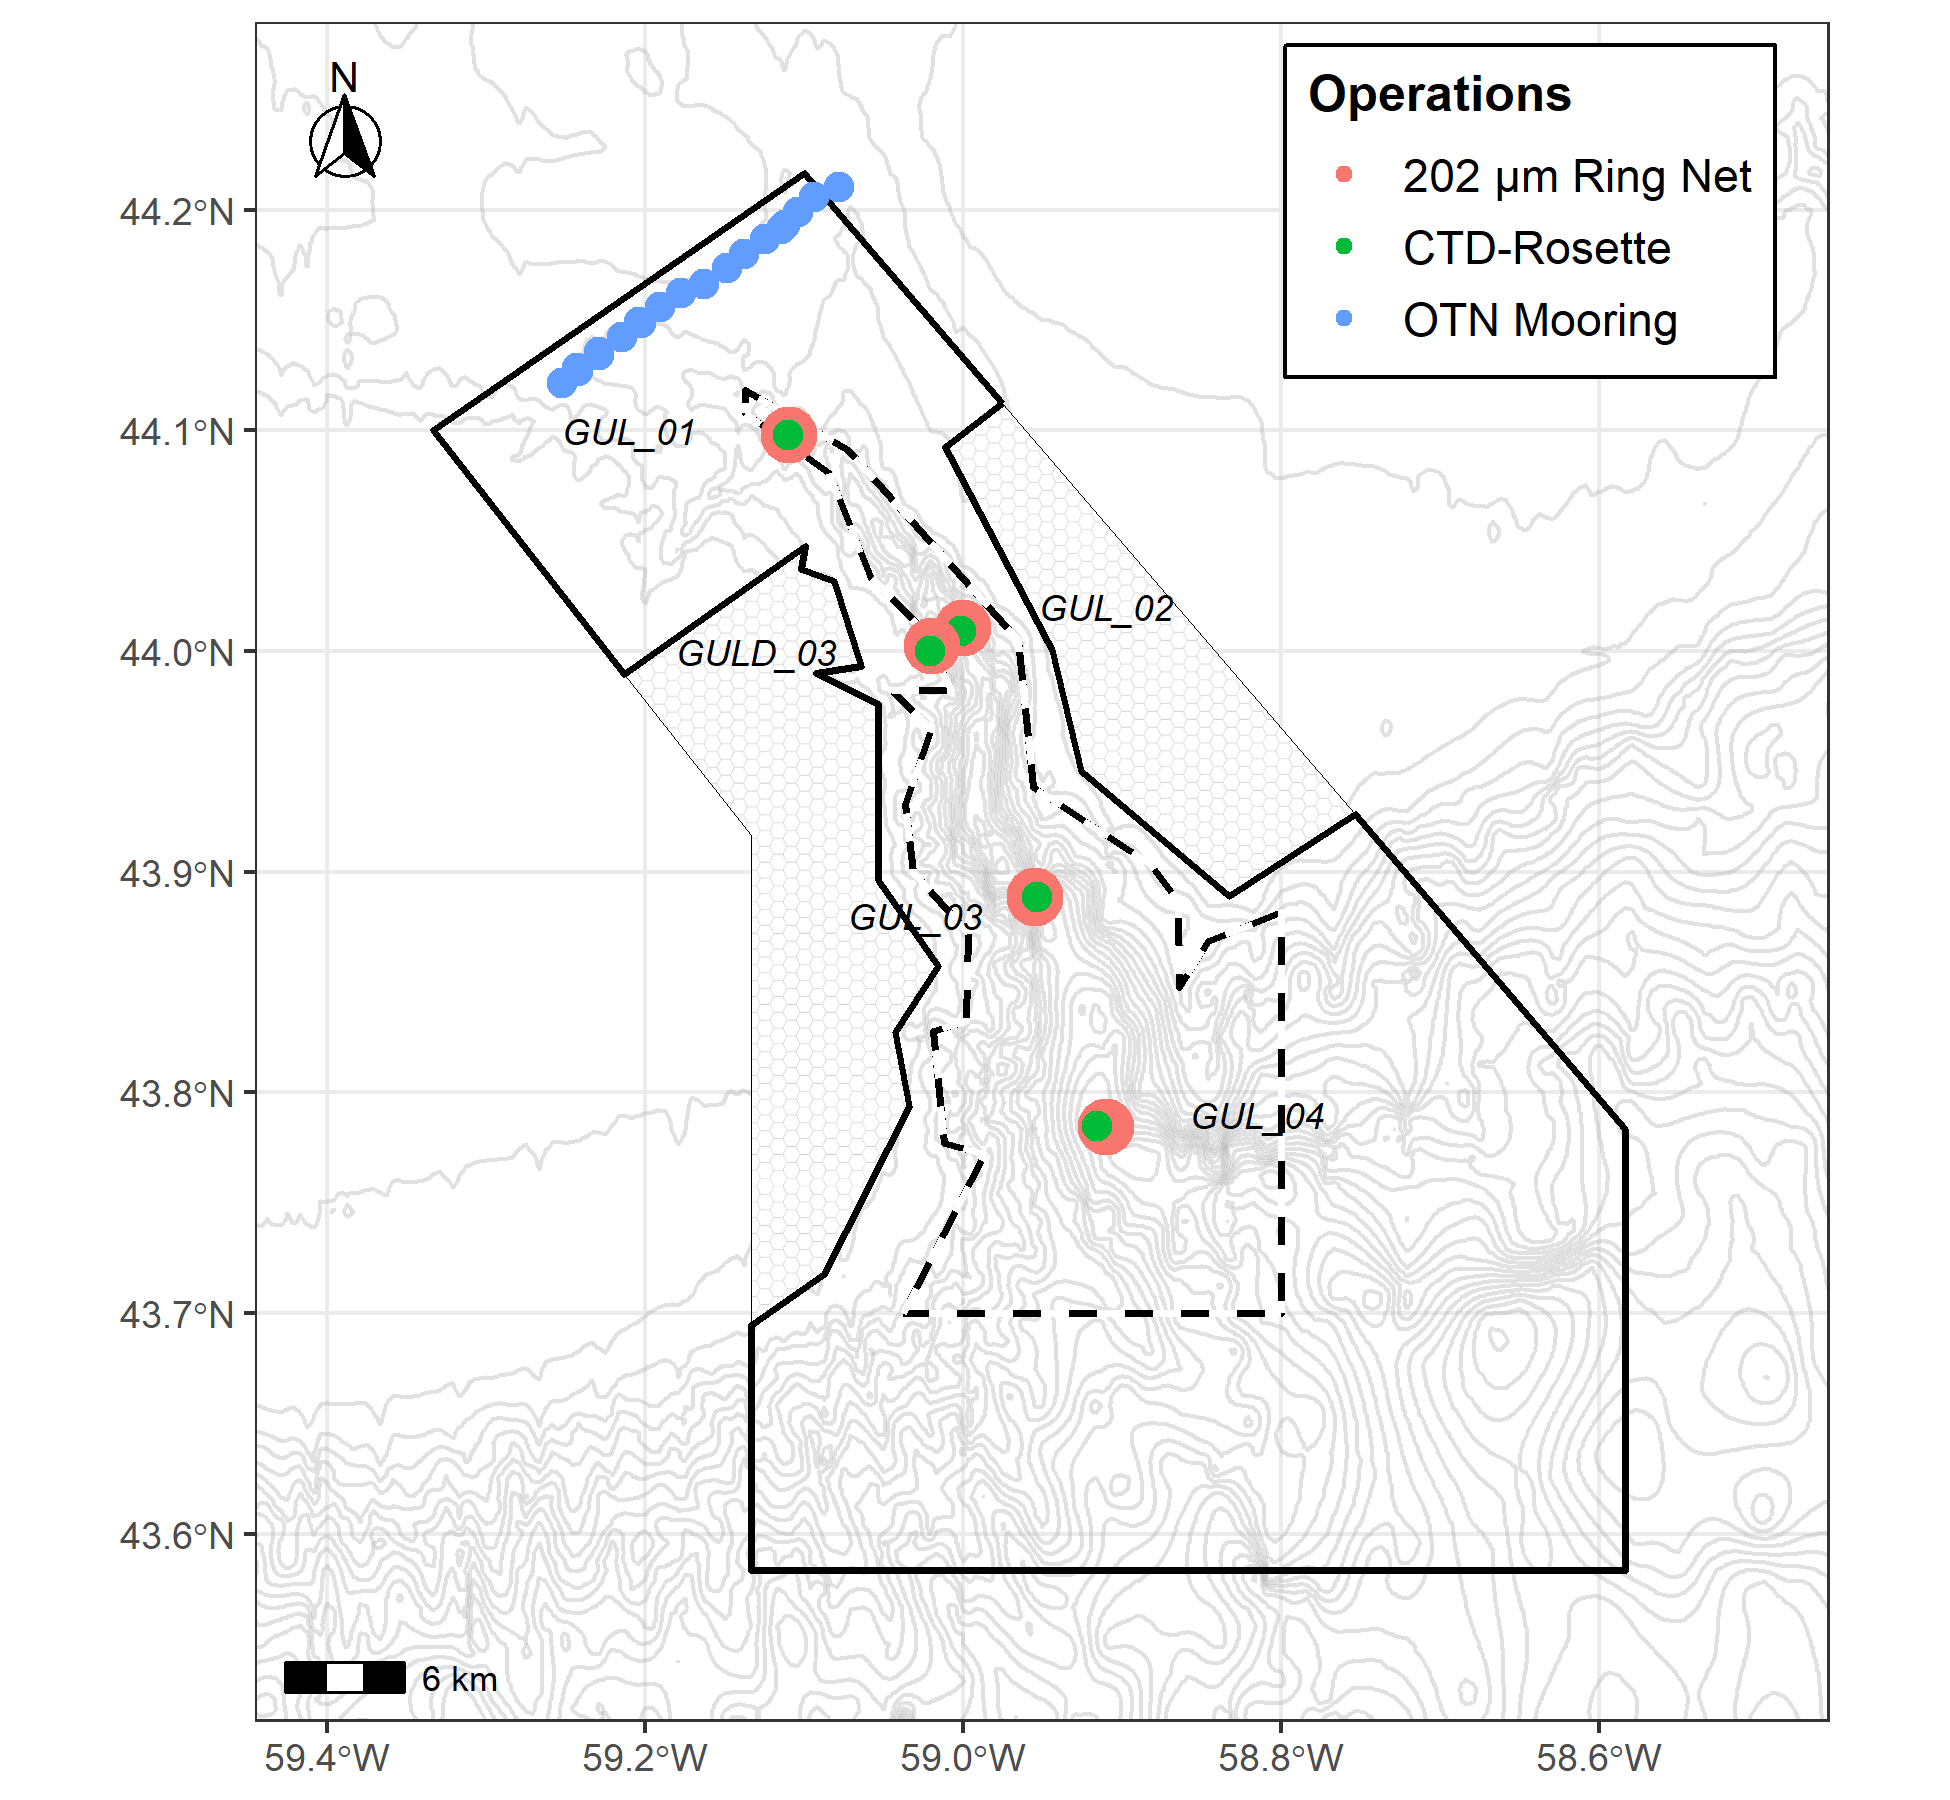
\includegraphics{knitr-figs-pdf/figure7-1} 

}

\caption{Location of Ocean Tracking Network acoustic receiver array partially recovered during the EN728 mission. Also shown are the boundaries and zones of the Gully Marine Protected Area, where the dashed line = Zone 1, solid line = Zone 2, hexagon pattern = Zone 3, and the Maritimes Region AZMP's CTD-Rosette and ring net monitoring stations.}\label{fig:figure7}
\end{figure}
\clearpage

\subsection{Shipboard Science Systems}\label{shipboard_systems}

\subsubsection{Vessel-Mounted Acoustic Doppler Current Profiler (VMADCP)}\label{vessel-mounted-acoustic-doppler-current-profiler-vmadcp}

Ocean currents were continuously measured throughout the EN728 mission using a dual vessel-mounted Acoustic Doppler Current Profiler (ADCP) system consisting of a 300 kHz RDI Workhorse Mariner and 75 kHz Ocean Surveyor ADCP systems. The transducers for these systems were mounted at \textasciitilde5 meters depth on the hull of the vessel. Data were processed on board in real time using the University of Hawaii's Data Acquisition System (UHDAS).

The 75 kHz ADCP reached \textasciitilde500-900 m depth in good weather in its deep-profiling mode, while the 300 kHz system reached to \textasciitilde90 m below the hull of the vessel. In bad weather, low scattering conditions, or some speed/heading/sea state conditions that entrain bubbles under the transducer, the range is less.

Data acquisition for the sonar and the requisite ancillary navigation streams occurs via the UHDAS software. An Ocean Surveyor is capable of running in either broadband mode (higher resolution at the expense of penetration) or narrowband mode (slightly deeper profiling but lower resolution). It is also capable of interweaving these pings. However, broadband mode was turned off during the EN728 mission and only narrowband mode was used. The ADCP system configuration in Table~\ref{tab:table8} remained consistent for the duration of the EN728 mission. Both ADCP systems were run continuously and simultaneously, except for when within the confines of the Gully MPA and when transiting across the boundaries of the Saint-Pierre et Miquelon Exclusive Economic Zone. Bottom tracking was turned on after departure for about half a day then remained off the remainder of the mission. A detailed digital log for the ADCPs was maintained by the URI marine technicians, which was sent together with the data to BIO Data Services Group for upload and archival in their protected server.

\hspace*{-0.5in}
\begin{table}[!h]
\centering
\caption{\label{tab:table8}Configuration settings for the 75 and 150 kHz VMADCP units on the RV \textit{Endeavor} for the 2025 spring AZMP mission (EN728).}
\centering
\begin{tabular}[t]{l>{\raggedright\arraybackslash}p{6em}>{\raggedright\arraybackslash}p{6em}>{\raggedright\arraybackslash}p{3em}>{\raggedright\arraybackslash}p{4em}>{\raggedright\arraybackslash}p{4em}>{\raggedright\arraybackslash}p{6em}}
\toprule
\begingroup\fontsize{12}{14}\selectfont \textbf{ADCP}\endgroup & \begingroup\fontsize{12}{14}\selectfont \textbf{Start Day}\endgroup & \begingroup\fontsize{12}{14}\selectfont \textbf{End Day}\endgroup & \begingroup\fontsize{12}{14}\selectfont \textbf{Ping}\endgroup & \begingroup\fontsize{12}{14}\selectfont \textbf{No. Bins}\endgroup & \begingroup\fontsize{12}{14}\selectfont \textbf{Bin Size (m)}\endgroup & \begingroup\fontsize{12}{14}\selectfont \textbf{Blank Distance (m)}\endgroup\\
\midrule
75 kHz & 2025-03-29 12:53:00 & 2025-04-18 11:56:00 & Narrow band & 100 & 8 & 8\\
150 kHz & 2025-03-29 12:53:00 & 2025-04-18 11:56:00 & Water profile & 35 & 4 & 4\\
\bottomrule
\end{tabular}
\end{table}
\clearpage

\subsubsection{Shipboard Flow-Through System and Meteorological Measurements}\label{shipboard-flow-through-system-and-meteorological-measurements}

The RV \emph{Endeavor} has uncontaminated science seawater that flowed into the vessel at \textasciitilde{} 5 metres depth into a seachest located in the engine room. This seawater was pumped via a non-metallic impeller pump past a SBE3S remote temperature sensor, through PVC piping and to outlets located in the Special Purpose and Wet Laboratories, and to the 01 deck. In the Wet Lab, the seawater flowed through a debubbler and was then split to a SBE21 TSG, SBE45 TSal, WET Labs WETStar chlorophyll fluorometer, ECO-Fluor fluorometer and the sink. The flowing water then drains overboard. This system also includes a surface PAR installed on the 01 deck of the vessel. Logging of these data was done using SBE Seasave software, and the resulting serial string were routed to NOAA's Scientific Computer System (SCS). From there, the Cruise Observations Real-time Interface and Open Live Information eXchange (CORIOLIX) system, accessed through shipboard LAN, was used to generate various data plots to visualize and inspect the collected data.

\subsubsection{Echosounders}\label{echosounders}

The RV \emph{Endeavor} is equipped with 12 kHz single-beam echosounder that was used for depth estimation during CTD and ring net operations. The echosounder ASCII string depth values and other data were routed to SCS. The vessel was also equipped with a low frequency 3.5 kHz echosounder (CHIRP), which was not used during the mission.

\subsubsection{Availability of Shipboard Data}\label{availability-of-shipboard-data}

All shipboard environmental data collected during the EN728 mission were archived at BIO in the ODIS data server and are available by request to \link{mailto:DFO.BIODataServices-BIOServicesdeDonnees.MPO@dfo-mpo.gc.ca}{\nolinkurl{DFO.BIODataServices-BIOServicesdeDonnees.MPO@dfo-mpo.gc.ca}}, and will also be submitted by the RV \emph{Endeavor} Marine Technical Services group to NSF-sponsored Rolling Deck to Repository \link{https://www.rvdata.us/}{R2R}. R2R catalogs and submits the underway environmental sensor data to long-term public archives, including the NOAA National Centers for Environmental Information (NCEI).

\clearpage

\section{Seabirds and Marine Mammal Observations}\label{seabirds-and-marine-mammal-observations}

\subsection{Background}\label{background-1}

The east coast of Canada supports millions of breeding marine birds as well as migrants from the southern hemisphere and the eastern North Atlantic. In 2005, the Canadian Wildlife Service (CWS) of Environment Canada initiated the Eastern Canada Seabirds at Sea (ECSAS) program with the goal of identifying and minimizing the impacts of human activities on birds in the marine environment. Since that time, a scientifically rigorous protocol for collecting data at sea and a sophisticated geodatabase have been developed, relationships with various industries and DFO to support offshore seabird observers have been established, and over 300,000 km of ocean track have been surveyed by CWS-trained observers. These data are now being used to quantify seabird abundance and distribution at sea and identify and mitigate any threats. In addition, data are collected on marine mammals, sea turtles, sharks, and other marine organisms when they are encountered.

\subsection{Methods}\label{methods}

Seabird surveys were conducted from the port side of the bridge of the RV \emph{Endeavor} during the EN728 mission. Surveys were conducted while the ship was moving at speeds greater than 4 knots, looking forward and scanning a 90° arc to one side of the ship. All birds observed on the water within a 300 m-wide transect were recorded, and we used the snapshot approach for flying birds (intermittent sampling based on the speed of the ship) to avoid overestimating abundance of birds flying in and out of transect. Distance sampling methods were incorporated to address the variation in bird detectability. Marine mammal and other marine wildlife observations were also recorded, although surveys were not specifically designed to detect marine mammals. Details of the methods used can be found in the CWS standardized protocol for pelagic seabird surveys from moving platforms (\citeproc{ref-Gjerdrum_2012}{Gjerdrum et al. 2012}).

\subsection{Results}\label{results}

A total of 1636.3 km of ocean was surveyed over 20 days. A total of 2469 marine birds were observed in transect (2786 in total) from 9 families (Table 1). Bird densities averaged 5.3 birds/km2 (ranging from 0 -- 449.3 birds/km2). The highest densities of birds (\textgreater{} 150 birds/km2) were observed at the shelf break on the Halifax Line, northeast of the Gully MPA, and the northwestern corner of Misaine Bank (Figure~\ref{fig:figure8}).

Sightings from the family Alcidae were the most abundant (53\% of the observations), most of which were Dovekie and Murre. Neither of these species breed in the area, but do spend a significant amount of time there during the non-breeding season. Laridae were also common (34\% of the observations), with Black-legged Kittiwake, Herring and Great Black-backed Gulls (Table~\ref{tab:table9}) observed throughout the survey area. An additional 12 terrestrial birds were observed offshore, either migrating overseas or blown off course (Table~\ref{tab:table10}). Only 26 marine mammals were observed during the surveys (Table~\ref{tab:table11}).

\subsection{The Gully and St.~Ann's Bank MPAs}\label{the-gully-and-st.-anns-bank-mpas}

Surveys took place in The Gully MPA on April 12 and 14 (see Figure~\ref{fig:figure8}) where a total of 44 marine birds were observed (Table~\ref{tab:table12}). Surveys in St.~Ann's Bank MPA took place on April 7-8, where 172 marine birds were sighting (Table~\ref{tab:table13}). No marine mammals were observed in either of the MPAs.

\vspace*{0.2in}


\begin{figure}[H]

{\centering \pdftooltip{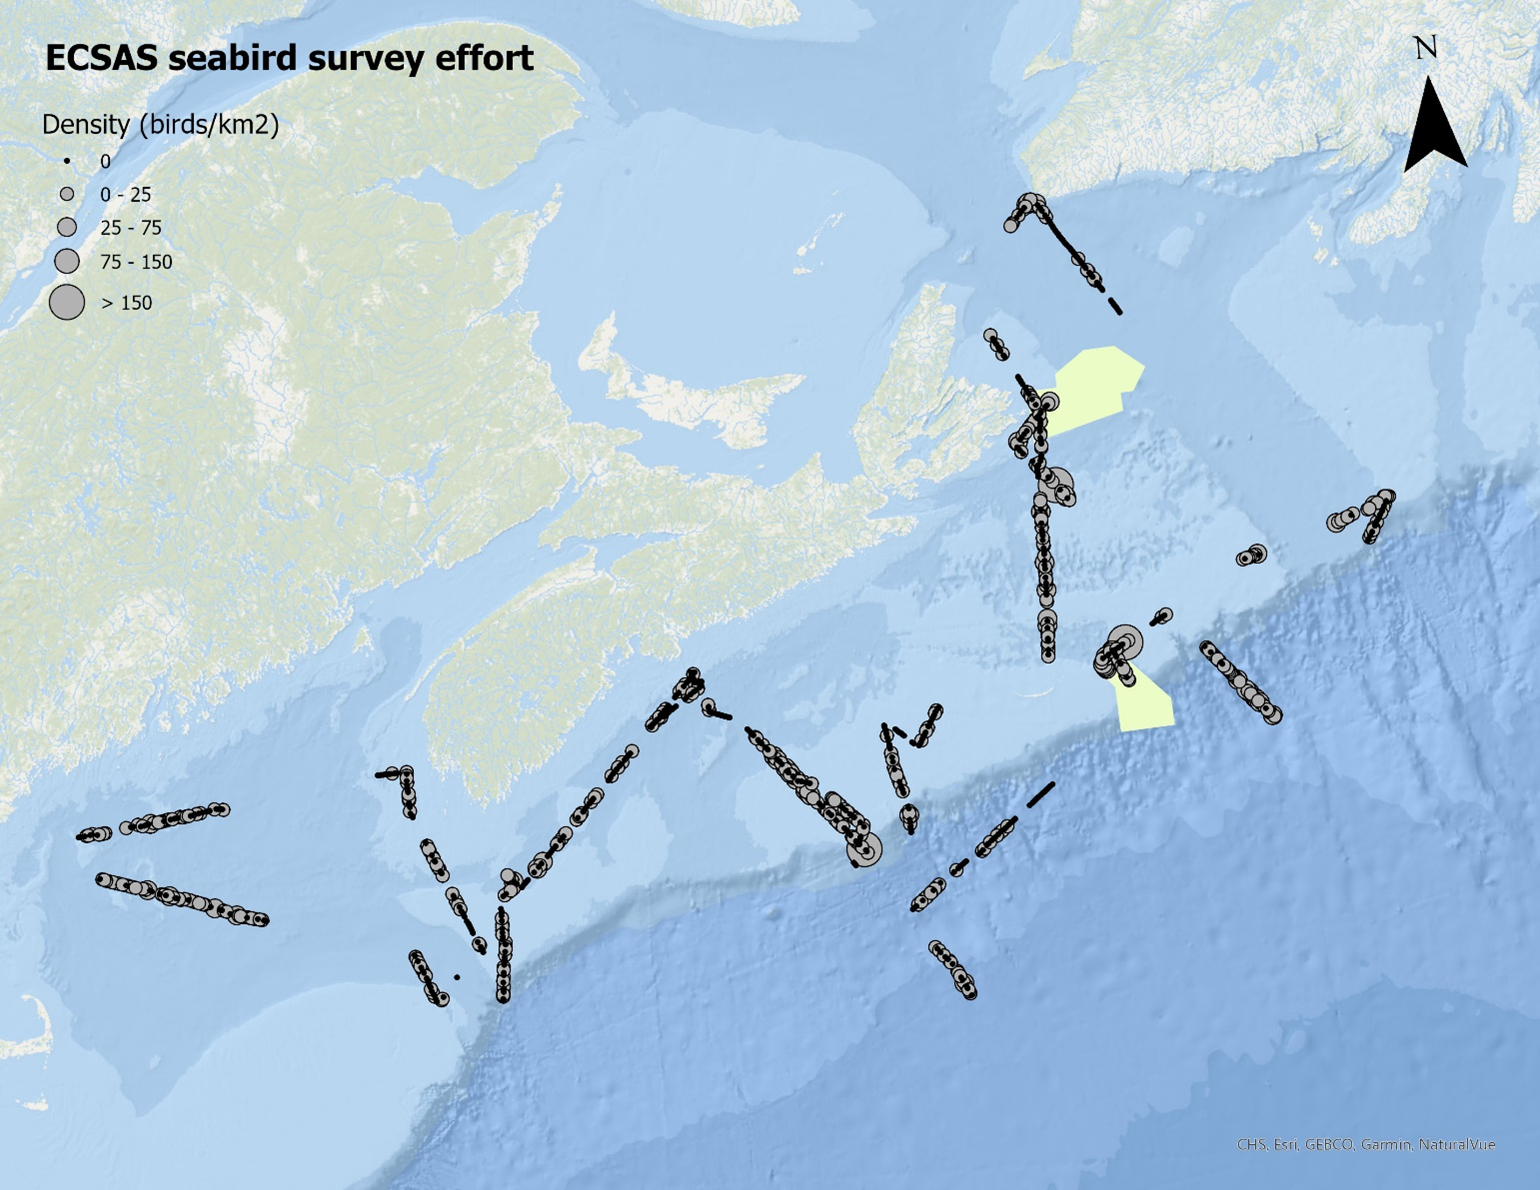
\includegraphics[width=5.13in]{figs/figure8}}{Figure} 

}

\caption{Density of birds (all species combined) observed during surveys on the Scotian Shelf AZMP from March 29 to April 17, 2025.}\label{fig:figure8}
\end{figure}
\clearpage
\begin{longtable}[t]{ll>{\raggedright\arraybackslash}p{11em}>{\raggedright\arraybackslash}p{3em}>{\raggedright\arraybackslash}p{4em}}
\caption{\label{tab:table9}List of marine bird species observed during surveys completed on the EN728 mission from from March 29 to April 17, 2025.}\\
\toprule
\begingroup\fontsize{12}{14}\selectfont \textbf{Family}\endgroup & \begingroup\fontsize{12}{14}\selectfont \textbf{Common Name}\endgroup & \begingroup\fontsize{12}{14}\selectfont \textbf{Latin}\endgroup & \begingroup\fontsize{12}{14}\selectfont \textbf{Total No.}\endgroup & \begingroup\fontsize{12}{14}\selectfont \textbf{No. Obs. in Transect}\endgroup\\
\midrule
\endfirsthead
\caption[]{\textit{(continued)}}\\
\toprule
\begingroup\fontsize{12}{14}\selectfont \textbf{Family}\endgroup & \begingroup\fontsize{12}{14}\selectfont \textbf{Common Name}\endgroup & \begingroup\fontsize{12}{14}\selectfont \textbf{Latin}\endgroup & \begingroup\fontsize{12}{14}\selectfont \textbf{Total No.}\endgroup & \begingroup\fontsize{12}{14}\selectfont \textbf{No. Obs. in Transect}\endgroup\\
\midrule
\endhead

\endfoot
\bottomrule
\endlastfoot
\begingroup\fontsize{11}{13}\selectfont \em{\textbf{Marine birds}}\endgroup & \begingroup\fontsize{11}{13}\selectfont \em{\textbf{}}\endgroup & \em{\begingroup\fontsize{11}{13}\selectfont \em{\textbf{}}\endgroup} & \begingroup\fontsize{11}{13}\selectfont \em{\textbf{}}\endgroup & \begingroup\fontsize{11}{13}\selectfont \em{\textbf{}}\endgroup\\
Gaviidae & Red-throated Loon & \em{Gavia stellata} & 1 & 0\\
Procellariidae & Northern Fulmar & \em{Fulmarus glacialis} & 53 & 53\\
 & Sooty Shearwater & \em{Ardenna grisea} & 24 & 23\\
 & Unidentified Shearwaters & \em{Puffinus or Calonectris or Ardenna} & 1 & 0\\
Hydrobatidae & Leach's Storm-Petrel & \em{Hydrobates leucorhous} & 20 & 17\\
 & Wilson's Storm Petrel & \em{Oceanites oceanicus} & 2 & 2\\
 & Unidentified Storm-Petrels & \em{Hydrobatidae} & 2 & 2\\
Phalacrocoracidae & Double-crested Cormorant & \em{Phalacrocorax auritus} & 9 & 9\\
 & Unidentified Cormorants & \em{Phalacrocorax} & 1 & 1\\
Sulidae & Northern Gannet & \em{Morus bassanus} & 200 & 196\\
Anatidae & Common Eider & \em{Somateria mollissima} & 27 & 25\\
 & Black Scoter & \em{Melanitta nigra} & 1 & 1\\
Scolopacidae & Unidentified Phalaropes & \em{Phalaropus} & 2 & 2\\
Laridae & Unidentified Skuas & \em{Stercorarius Skuas} & 20 & 20\\
 & Black-legged Kittiwake & \em{Rissa tridactyla} & 145 & 145\\
 & Herring Gull & \em{Larus argentatus} & 115 & 107\\
 & Great Black-backed Gull & \em{Larus marinus} & 107 & 106\\
 & Ring-billed Gull & \em{Larus delawarensis} & 85 & 83\\
 & Iceland Gull & \em{Larus glaucoides} & 5 & 5\\
 & Glaucous Gull & \em{Larus hyperboreus} & 3 & 3\\
 & Unidentified Gulls & \em{Larus} & 635 & 357\\
 & Unidentified Terns & \em{Sterna} & 19 & 15\\
Alcidae & Dovekie & \em{Alle alle} & 509 & 507\\
 & Common Murre & \em{Uria aalge} & 66 & 63\\
 & Thick-billed Murre & \em{Uria lomvia} & 38 & 38\\
 & Unidentified Murres & \em{Uria} & 328 & 321\\
 & Atlantic Puffin & \em{Fratercula arctica} & 33 & 33\\
 & Razorbill & \em{Alca torda} & 12 & 12\\
 & Black Guillemot & \em{Cepphus grylle} & 4 & 4\\
 & Unidentified Auks & \em{Alcidae} & 319 & 319\\
\begingroup\fontsize{11}{13}\selectfont \textbf{Total}\endgroup & \begingroup\fontsize{11}{13}\selectfont \textbf{}\endgroup & \em{\begingroup\fontsize{11}{13}\selectfont \textbf{}\endgroup} & \begingroup\fontsize{11}{13}\selectfont \textbf{2786}\endgroup & \begingroup\fontsize{11}{13}\selectfont \textbf{2469}\endgroup\\*
\end{longtable}
\clearpage
\begin{longtable}[t]{>{\raggedright\arraybackslash}p{8em}l>{\raggedright\arraybackslash}p{10em}>{\raggedright\arraybackslash}p{3em}}
\caption{\label{tab:table10}List of terrestrial bird species observed during surveys completed on the EN728 mission from from March 29 to April 17, 2025.}\\
\toprule
\begingroup\fontsize{12}{14}\selectfont \textbf{Family}\endgroup & \begingroup\fontsize{12}{14}\selectfont \textbf{Common Name}\endgroup & \begingroup\fontsize{12}{14}\selectfont \textbf{Latin}\endgroup & \begingroup\fontsize{12}{14}\selectfont \textbf{Total No.}\endgroup\\
\midrule
\endfirsthead
\caption[]{\textit{(continued)}}\\
\toprule
\begingroup\fontsize{12}{14}\selectfont \textbf{Family}\endgroup & \begingroup\fontsize{12}{14}\selectfont \textbf{Common Name}\endgroup & \begingroup\fontsize{12}{14}\selectfont \textbf{Latin}\endgroup & \begingroup\fontsize{12}{14}\selectfont \textbf{Total No.}\endgroup\\
\midrule
\endhead

\endfoot
\bottomrule
\endlastfoot
\begingroup\fontsize{11}{13}\selectfont \em{\textbf{Terrestrial birds}}\endgroup & \begingroup\fontsize{11}{13}\selectfont \em{\textbf{}}\endgroup & \em{\begingroup\fontsize{11}{13}\selectfont \em{\textbf{}}\endgroup} & \begingroup\fontsize{11}{13}\selectfont \em{\textbf{}}\endgroup\\
Emberizidae & Unidentified Sparrows & \em{Emberizidae} & 6\\
 & Dark-eyed Junco & \em{Junco hyemalis} & 1\\
Regulidae & Golden-crowned Kinglet & \em{Regulus satrapa} & 2\\
Picidae & Northern Flicker & \em{Colaptes auratus} & 1\\
 & Unknown Bird & \em{Aves} & 2\\
\begingroup\fontsize{11}{13}\selectfont \textbf{Total}\endgroup & \begingroup\fontsize{11}{13}\selectfont \textbf{}\endgroup & \em{\begingroup\fontsize{11}{13}\selectfont \textbf{}\endgroup} & \begingroup\fontsize{11}{13}\selectfont \textbf{12}\endgroup\\*
\end{longtable}
\begin{longtable}[t]{>{\raggedright\arraybackslash}p{12em}>{\raggedright\arraybackslash}p{9em}>{\raggedright\arraybackslash}p{4em}}
\caption{\label{tab:table11}List of non-avian species observed during surveys completed on the EN728 mission from from March 29 to April 17, 2025.}\\
\toprule
\begingroup\fontsize{12}{14}\selectfont \textbf{Common Name}\endgroup & \begingroup\fontsize{12}{14}\selectfont \textbf{Latin}\endgroup & \begingroup\fontsize{12}{14}\selectfont \textbf{Total No.}\endgroup\\
\midrule
\endfirsthead
\caption[]{\textit{(continued)}}\\
\toprule
\begingroup\fontsize{12}{14}\selectfont \textbf{Common Name}\endgroup & \begingroup\fontsize{12}{14}\selectfont \textbf{Latin}\endgroup & \begingroup\fontsize{12}{14}\selectfont \textbf{Total No.}\endgroup\\
\midrule
\endhead

\endfoot
\bottomrule
\endlastfoot
\begingroup\fontsize{11}{13}\selectfont \em{\textbf{Marine mammals}}\endgroup & \em{\begingroup\fontsize{11}{13}\selectfont \em{\textbf{}}\endgroup} & \begingroup\fontsize{11}{13}\selectfont \em{\textbf{}}\endgroup\\
Harbour Porpoise & \em{Phocoena phocoena} & 5\\
Bottlenose Dolphin & \em{Tursiops truncatus} & 2\\
Long-finned Pilot Whale & \em{Globicephala melas} & 15\\
Unidentified cetacean & \em{Cetacea} & 3\\
Unidentified seal & \em{Phocidae} & 1\\
\begingroup\fontsize{11}{13}\selectfont \textbf{Total}\endgroup & \em{\begingroup\fontsize{11}{13}\selectfont \textbf{}\endgroup} & \begingroup\fontsize{11}{13}\selectfont \textbf{26}\endgroup\\*
\end{longtable}
\clearpage
\begin{longtable}[t]{>{\raggedright\arraybackslash}p{13em}>{\raggedright\arraybackslash}p{10em}>{\raggedright\arraybackslash}p{4em}}
\caption{\label{tab:table12}List of marine bird species observed during surveys within The Gully MPA on April 12 and 14, 2025 during the EN728 mission}\\
\toprule
\begingroup\fontsize{12}{14}\selectfont \textbf{Common Name}\endgroup & \begingroup\fontsize{12}{14}\selectfont \textbf{Latin}\endgroup & \begingroup\fontsize{12}{14}\selectfont \textbf{Total No.}\endgroup\\
\midrule
\endfirsthead
\caption[]{\textit{(continued)}}\\
\toprule
\begingroup\fontsize{12}{14}\selectfont \textbf{Common Name}\endgroup & \begingroup\fontsize{12}{14}\selectfont \textbf{Latin}\endgroup & \begingroup\fontsize{12}{14}\selectfont \textbf{Total No.}\endgroup\\
\midrule
\endhead

\endfoot
\bottomrule
\endlastfoot
Unidentified Murres & \em{Uria} & 9\\
Unidentified Auks & \em{Alcidae} & 8\\
Common Murre & \em{Uria allge} & 8\\
Black-legged Kittiwake & \em{Rissa tridactyla} & 5\\
Black Guillemot & \em{Cepphus grylle} & 4\\
Great Black-backed Gull & \em{Larus marinus} & 4\\
Atlantic Puffin & \em{Fratercula arctica} & 3\\
Common Eider & \em{Somateria mollissima} & 2\\
Thick-billed Murre & \em{Uria lomvia} & 1\\
\begingroup\fontsize{11}{13}\selectfont \textbf{Total}\endgroup & \em{\begingroup\fontsize{11}{13}\selectfont \textbf{}\endgroup} & \begingroup\fontsize{11}{13}\selectfont \textbf{44}\endgroup\\*
\end{longtable}
\begin{longtable}[t]{>{\raggedright\arraybackslash}p{10em}>{\raggedright\arraybackslash}p{10em}>{\raggedright\arraybackslash}p{4em}}
\caption{\label{tab:table13}List of marine bird species observed during surveys within the St. Anns Bank MPA on April 7 and 8, 2025 during the EN728 mission}\\
\toprule
\begingroup\fontsize{12}{14}\selectfont \textbf{Common Name}\endgroup & \begingroup\fontsize{12}{14}\selectfont \textbf{Latin}\endgroup & \begingroup\fontsize{12}{14}\selectfont \textbf{Total No.}\endgroup\\
\midrule
\endfirsthead
\caption[]{\textit{(continued)}}\\
\toprule
\begingroup\fontsize{12}{14}\selectfont \textbf{Common Name}\endgroup & \begingroup\fontsize{12}{14}\selectfont \textbf{Latin}\endgroup & \begingroup\fontsize{12}{14}\selectfont \textbf{Total No.}\endgroup\\
\midrule
\endhead

\endfoot
\bottomrule
\endlastfoot
Unidentified Murres & \em{Uria} & 54\\
Black-legged Kittiwake & \em{Rissa tridactyla} & 35\\
Unidentified Auks & \em{Alcidae} & 26\\
Herring Gull & \em{Larus argentatus} & 11\\
Northern Fulmar & \em{Fulmarus glacialis} & 9\\
Common Murre & \em{Uria aalge} & 8\\
Northern Gannet & \em{Morus bassanus} & 8\\
Ring-billed Gull & \em{Larus delawarensis} & 5\\
Unidentified Gulls & \em{Larus} & 8\\
Thick-billed Murre & \em{Uria lomvia} & 3\\
Leach's Storm-Petrel & \em{Oceanodroma leucorhoa} & 1\\
Razorbill & \em{Alca torda} & 1\\
Sooty Shearwater & \em{Ardenna griseus} & 1\\
Unidentified Terns & \em{Sterna} & 1\\
Great Black-backed Gull & \em{Larus marinus} & 1\\
\begingroup\fontsize{11}{13}\selectfont \textbf{Total}\endgroup & \em{\begingroup\fontsize{11}{13}\selectfont \textbf{}\endgroup} & \begingroup\fontsize{11}{13}\selectfont \textbf{172}\endgroup\\*
\end{longtable}
\clearpage

\section{Data Management Summary}\label{DM}

\subsection{Metadata Collection and Archival}\label{metadata-collection-and-archival}

Both digital and paper logs were used to record sample and event metadata during the EN728 mission. Paper logs included CTD `deck' sheets, ring net, mooring, Argo float, chlorophyll laboratory log and underway sample log. ELOG, an electronic logbook system for collecting event metadata, was used to log the time, ship's position, and sounding associated with certain logistical aspects of each gear deployment (e.g., deployed, on bottom, and recovered). This electronic logbook was accessible on the ship's network and mobile devices. In addition an ELOG observations log was used to record detailed comments and observations on cruise activities and an underway log was used to record the samples collected, time and position. The ELOG configuration, deployment and backup was managed using Git locally, and was pushed to GitHub upon return (\url{https://github.com/dfo-mar-odis/azmp_elog/tree/EN728}). The recording of metadata in ELOG facilitates the upload of discrete and plankton data to the BioChem repository.

ELOG was run from a Windows 10 laptop in the Main Laboratory near the CTD acquisition computer, while a second laptop was placed in the Wet Laboratory to assist the ring net operator in logging their events. The GPS and sounder feed for ELOG from the ship's network was read using Python scripts called from the ELOG configuration file. Two tablets were used to access ELOG while conducting ring net operations on the starboard deck.

Digital filtration logs were used by laboratory staff for logging details associated with the processing of collected water. These filtration logs are generated using the R statistical software from the planned water budget for each station. A laptop was placed in the Main Laboratory to facilitate the access and modification of these digital filtration logs.

All digital data were backed up at least daily on the network or on an external hard drive. At the end of the mission all data were copied and paper logs were scanned and sent to BIO Data Services for upload and archival into their protected server.

\subsection{DFO At-sea Reporting Template (DART)}\label{dfo-at-sea-reporting-template-dart}

The in-house DFO At-sea Reporting Template \link{https://github.com/dfo-mar-odis/dart}{DART} was used to compile and reformat all discrete data collected and analyzed at sea (dissolved oxygen, chlorophyll, and salinity) to check the data and facilitate later processing and archiving. This process involved loading the ELOG files, the CTD bottle (.btl) files containing and the discrete bottle measurements. DART was also used to produce reports of the linked bottle and sensor measurements, to facilitate the quality control of both sensor and bottle measurements while at sea.

\subsection{Data Submission to Global Telecommunications Systems}\label{data-submission-to-global-telecommunications-systems}

Global Telecommunications Systems (GTS) houses oceanographic data for the primary purpose of weather forecasting. However, the data are also available for modellers to assimilate into their climate forecasting. DFO's representative in GTS is Environment and Climate Change Canada.

AZMP submits CTD data to GTS via MEDS (Marine Environmental Data Section, Ocean Sciences Division, DFO) at regular intervals throughout each mission to \link{mailto:MEDS-SDMM.XNCR@dfo-mpo.gc.ca}{\nolinkurl{MEDS-SDMM.XNCR@dfo-mpo.gc.ca}}. The data must be sent within 30 days of collection. The files submitted are a customized .txt file called an IGOSS file, which is generated using the in-house CTD post-processing software CTDDAP.

\clearpage

\section{Operational Considerations and Issues of Note}\label{operation-issues}

This section contains a brief summary of the various operational considerations or issues encountered with science equipment and/or data and sample post-processing during the EN728 mission. This information should help to guide both CTD and laboratory post-processing procedures, and future interpretation of the data collected on the mission.

\subsection{CTD Operations}\label{ctd-operations-1}
\begin{enumerate}
\def\labelenumi{\arabic{enumi}.}
\item
  The CTD standard operating procedure used during CTD data acquisition from Events 001 to 061 differed slightly between CTD computer operators on the day (07:00-19:00) and night (19:00-07:00) shifts. For casts collected during the day shift, the CTD deck box was turned on only after the CTD-Rosette was deployed and resting at its 10-m soak depth. While this appeared to have no issue on the resulting cast data and removal of the soak from the downcast, this procedure was changed starting on Event 062 so that the deck unit was turned on just prior to the initial deployment of the CTD-Rosette system, so that the procedures were consistent between day and night shift deployments.
\item
  Several Niskin bottle misfires occurred throughout the mission. In some cases these misfires were consistently from the same bottle, which was mitigated by changing the bottle position on the rosette, or by changing trigger mechanism. In all cases, these misfires occurred at depths where water samples were collected in duplicate, which provided enough water to satisfy the amount of samples collected by both DFO and Dalhousie University science staff. Thus no samples were lost as a result of these misfires. Comments related to bottle misfires were captured in the ELOG Comments field presented in Table~\ref{tab:table3}.
\end{enumerate}
\subsection{Ring Net Operations}\label{ring-net-operations}
\begin{enumerate}
\def\labelenumi{\arabic{enumi}.}

\item
  Ring net operations were aborted and re-deployed at several stations (PL\_06, NEC\_04, and GUL\_03) due to the crossbow sliding down the wire, invalidating the sample. In all cases, the net was re-deployed successfully after the crossbow was re-adjusted and tightened on the wire. This issue was more prominent when using one particular crossbow that had a slightly smaller groove for the wire on its top clamp. At station HL\_01, the PVC cap fell off the cod end of the net, resulting in the loss of the sample upon recovery. At station STAB\_05, the winch wire rubbed against the vessel's winch cab (known as the `dog house'), and the net descent was paused for a long duration at 200 m. It was decided to recover the net and re-deploy.
\end{enumerate}
\subsection{Mooring Operations}\label{mooring-operations-1}
\begin{enumerate}
\def\labelenumi{\arabic{enumi}.}

\item
  The acoustic receiver moorings at stations GUL02, GUL03, and GUL05 could not be recovered during the mission. The status of the receivers at stations GUL02 and GUL03 showed a tilt ranging between 56-58\(^\circ\) and 68-79\(^\circ\), respectively, suggesting they were laying near-horizontal on the seabed. Communications could not be established with the release at station GUL05.
\end{enumerate}
\subsection{Flow-Through System}\label{flow-through-system}
\begin{enumerate}
\def\labelenumi{\arabic{enumi}.}

\item
  The BIO flow-through system was initially connected to the vessel's uncontaminated science seawater outflow modulated by an impeller pump. However, on April 6 it was noticed that the outflow from the system had suddenly stopped. The power to the pump was evaluated by the vessel's engineers and turned back on. On April 9 and again on April 10, the impeller pump had shut off again unexpectedly. As these shut offs became more frequent, a decision was made to switch the BIO flow-through system to the science seawater modulated by the vessel's diaphragm pump on April 14. The disruption and shut down of the impeller pump also affected the only intake temperature sensor for both science seawater pumps, which is inline with the impeller pump. Consequently, the intake temperature for the BIO flow-through system was switched to a temperature sensor located on the transducer. The depth of this sensor is 5 m below sea surface, and was considered comparable to the impeller pump intake temperature.
\end{enumerate}
\clearpage

\section{Acknowledgements}\label{acks}

We would like to thank all science staff of the EN728 mission for their dedication and hard work to make the mission a success. We also thank Commanding Officer Christopher Armanetti, as well as the officers, crew, and marine technicians of the RV \emph{Endeavor} for their dedication and support during the mission.

We thank Jay Barthelotte, Regional Vessel Coordinator, DFO Maritimes Region, for coordinating the logistics of the vessel's scheduling and arrival. We would like to thank Jennifer Field, Mike Vining, and Katie Warman (Ocean Engineering and Technology Section, DFO) for their assistance in the mobilization and/or demobilization of the science equipment used on the mission. We thank Dennis McGillicuddy and Mike Brosnahan (WHOI) for facilitating the installation of the IFCB system on board.

We would also like to thank xxxx and xxxx (DFO OESD) for their review of this report. This document was produced using the \link{https://github.com/pbs-assess/csasdown?tab=readme-ov-file}{csasdown R package} using RStudio version 2023.12.0 (R Core Team, 2023).

Funding for this mission was provided by DFO's National Science At-Sea Program.

\clearpage

\section{References}\label{references}

\phantomsection\label{refs}
\begin{CSLReferences}{1}{1}
\bibitem[\citeproctext]{ref-Beazley_2024}
Beazley, L., Cardoso, D., Gordon, C., and Gjerdrum, C. 2024. \link{https://waves-vagues.dfo-mpo.gc.ca/library-bibliotheque/41269986.pdf}{Mission report for the maritimes region atlantic zone monitoring program 2024 spring survey (TEL2024880).} Can. Tech. Rep. Hydrogr. Ocean Sci. 386: vii 102~p.

\bibitem[\citeproctext]{ref-Cetinic_2016}
Cetinić, I., Poulton, N., and Slade, W.H. 2016. \link{https://doi.org/10.1364/OE.24.020703}{Characterizing the phytoplankton soup: Pump and plumbing effects on the particle assemblage in underway optical seawater systems.} Optics Express 24(18): 13~pp.

\bibitem[\citeproctext]{ref-Devine_2014}
Devine, L., Kennedy, M.K., St-Pierre, I., Lafleur, C., Ouellet, M., and Bond, S. 2014. \link{https://waves-vagues.dfo-mpo.gc.ca/library-bibliotheque/351319.pdf}{BioChem: The fisheries and oceans canada database for biological and chemical data.} Can. Tech. Rep. Fish. Aquat. Sci. 3073: iv + 40~p.

\bibitem[\citeproctext]{ref-Dickson_2007}
Dickson, A.G., Sabine, C.L., and Christian (Eds.)., J.R. 2007. \link{https://www.nodc.noaa.gov/ocads/oceans/Handbook_2007.html}{Guide to best practices for ocean CO2 measurements.} PICES Special Publication 3: 191~p.

\bibitem[\citeproctext]{ref-Gjerdrum_2012}
Gjerdrum, C., Fifield, D.A., and Wilhelm, S.I. 2012. \link{https://publications.gc.ca/collections/collection_2012/ec/CW69-5-515-eng.pdf}{Eastern canada seabirds at sea (ECSAS) standardized protocol for pelagic seabird surveys from moving and stationary platforms.} Can. Wildl. Serv. Tech. Rep. Ser. No. 515: vi + 37~pp.

\bibitem[\citeproctext]{ref-Head_1992}
Head, E.J.H., and Harris, L.R. 1992. \link{https://www.int-res.com/articles/meps/86/m086p229.pdf}{Chlorophyll and carotenoid transformation and destruction by {\emph{Calanus}} spp. Grazing on diatoms.} Mar. Ecol. Prog. Ser. 86: 229--238.

\bibitem[\citeproctext]{ref-Hoepffner_1992}
Hoepffner, N., and Sathyendranath, S. 1992. \link{https://doi.org/10.4319/lo.1992.37.8.1660}{Bio-optical characteristics of coastal waters: Absorption spectra of phytoplankton and pigment distribution in the western north atlantic.} Limnol. Ocean. 37(8): 1660--1679.

\bibitem[\citeproctext]{ref-Hoepffner_1993}
Hoepffner, N., and Sathyendranath, S. 1993. \link{https://doi.org/10.1029/93JC01273}{Determination of the major groups of phytoplankton pigments from the absorption spectra of total particulate matter.} J. Geophys. Res. 98(C12): 22789--22803.

\bibitem[\citeproctext]{ref-Li_2001}
Li, B., and Dickie, P.M. 2001. \link{https://doi.org/10.1002/1097-0320(20010701)44:3\%3C236::AID-CYTO1116\%3E3.0.CO;2-5}{Monitoring phytoplankton, bacterioplankton, and virioplankton in a coastal inlet (bedford basin) by flow cytometry.} Cytometry. 44: 236--246.

\bibitem[\citeproctext]{ref-Mannino_2019}
Mannino, A., Novak, M.G., Nelson, N.B., Belz, M., Berthon, N.V., Blough, E.J., Boss, E., Bricaud, A., Chaves, J., Del Castillo, C., Del Vecchio, R., D'Sa, E.J., Freeman, S., Matsuoka, A., Miller, R.L., R., N.A., Röttgers, R., Tzortziou, M., and Werdell, P.J. 2019. \link{https://ioccg.org/wp-content/uploads/2019/10/cdom_abs_protocol_public_draft-19oct-2019-sm.pdf}{Measurement protocol of absorption by chromophoric dissolved organic matter (CDOM) and other dissolved materials.} \emph{In} Inherent optical property measurements and protocols: Absorption coefficient. IOCCG, Dartmouth, NS, Canada.

\bibitem[\citeproctext]{ref-Mitchell_2002}
Mitchell, M.R., Harrison, G., Kevin, K., Gagné, A., Maillet, G., and Strain, P. 2002. \link{https://waves-vagues.dfo-mpo.gc.ca/library-bibliotheque/265754.pdf}{Atlantic zonal monitoring program sampling protocol.} Can. Tech. Rep. Fish. Hydrogr. Ocean Sci. 223: iv + 23~p.

\bibitem[\citeproctext]{ref-SBE_2024a}
Scientific, S.-B. 2024a. \link{https://www.seabird.com/sbe-4-conductivity-sensor/product-downloads?id=60762467707}{Calculate temperature and conductivity slope and offset correction coefficients. Application note 31.}

\bibitem[\citeproctext]{ref-SBE_2024b}
Scientific, S.-B. 2024b. \link{https://www.seabird.com/sbe-43-dissolved-oxygen-sensor/product-downloads?id=60762467728/}{SBE 43 DO sensor calibration and data corrections. Application note 64-2.}

\bibitem[\citeproctext]{ref-wong2020}
Wong, A.P., Wijffels, S.E., Riser, S.C., Pouliquen, S., Hosoda, S., Roemmich, D., Gilson, J., Johnson, G.C., Martini, K., Murphy, D.J., and al., et. 2020. \link{https://doi.org/10.3389/fmars.2020.00700}{Argo data 1999-2019: Two million temperature-salinity profiles and subsurface velocity observations from a global array of profiling floats}. Frontiers in Marine Science 7.

\end{CSLReferences}
\noindent \vspace{-2em} \setlength{\leftskip}{0.2in} \setlength{\parskip}{8pt} \vspace{-2em}

\clearpage

\begin{appendices}
\counterwithin{figure}{section}
\counterwithin{table}{section}
\counterwithin{equation}{section}

\pagestyle{plain}

\section{Vertical Profiles of Temperature, Salinity, Dissolved Oxygen}\label{appA}

This appendix illustrates the vertical profiles of temperature, salinity, and dissolved oxygen for each station sampled during the EN728 mission. Profile plots are organized by hydrographic section (e.g., Halifax Line). These plots were generated routinely throughout the mission and compared against the corresponding bottle salinity and dissolved oxygen measurements obtained via Winkler titrations as a tool to A) evaluate any discrepancies between the dual sensors, B) evaluate which of the dual sensors more closely reflected the corresponding bottle measurements generated at sea, a task which helps guide the final sensor calibration process, and C) evaluate the laboratory measurements for visual outliers. Outliers in the bottle data were identified based on their divergence from replicate samples, when collected, or whether they fell far from the CTD profile data, and were assigned quality control flags according to the quality control flag schema applied to data submitted in DFO's National Repository, BioChem (\citeproc{ref-Devine_2014}{Devine et al. 2014}).

For the majority of the casts conducted during the mission there was excellent congruence between both the primary and secondary dissolved oxygen and conductivity sensors, and between the sensor and bottle data. Although data from the primary and secondary oxygen sensors were comparable, the secondary sensor was closer to the corresponding Winkler titration values than the primary.

Although bottle chlorophyll measurements are not used to calibrate the sensor data, they were routinely compared against the chlorophyll fluorometer sensor data throughout the mission to evaluate the reliability of the sensor, and to ensure that all bottle sample IDs for parameters measured at sea were accounted for. The discrepancy between the sensor data and bottle measurements was higher, especially at the depth of the chlorophyll maximum, where the sensors underestimated chlorophyll concentration relative to the bottle measurements. Consequently, outliers were assigned to bottle measurements based only on their deviation from replicate bottle values, and not the sensor data.
\begin{figure}[H]

{\centering \pdftooltip{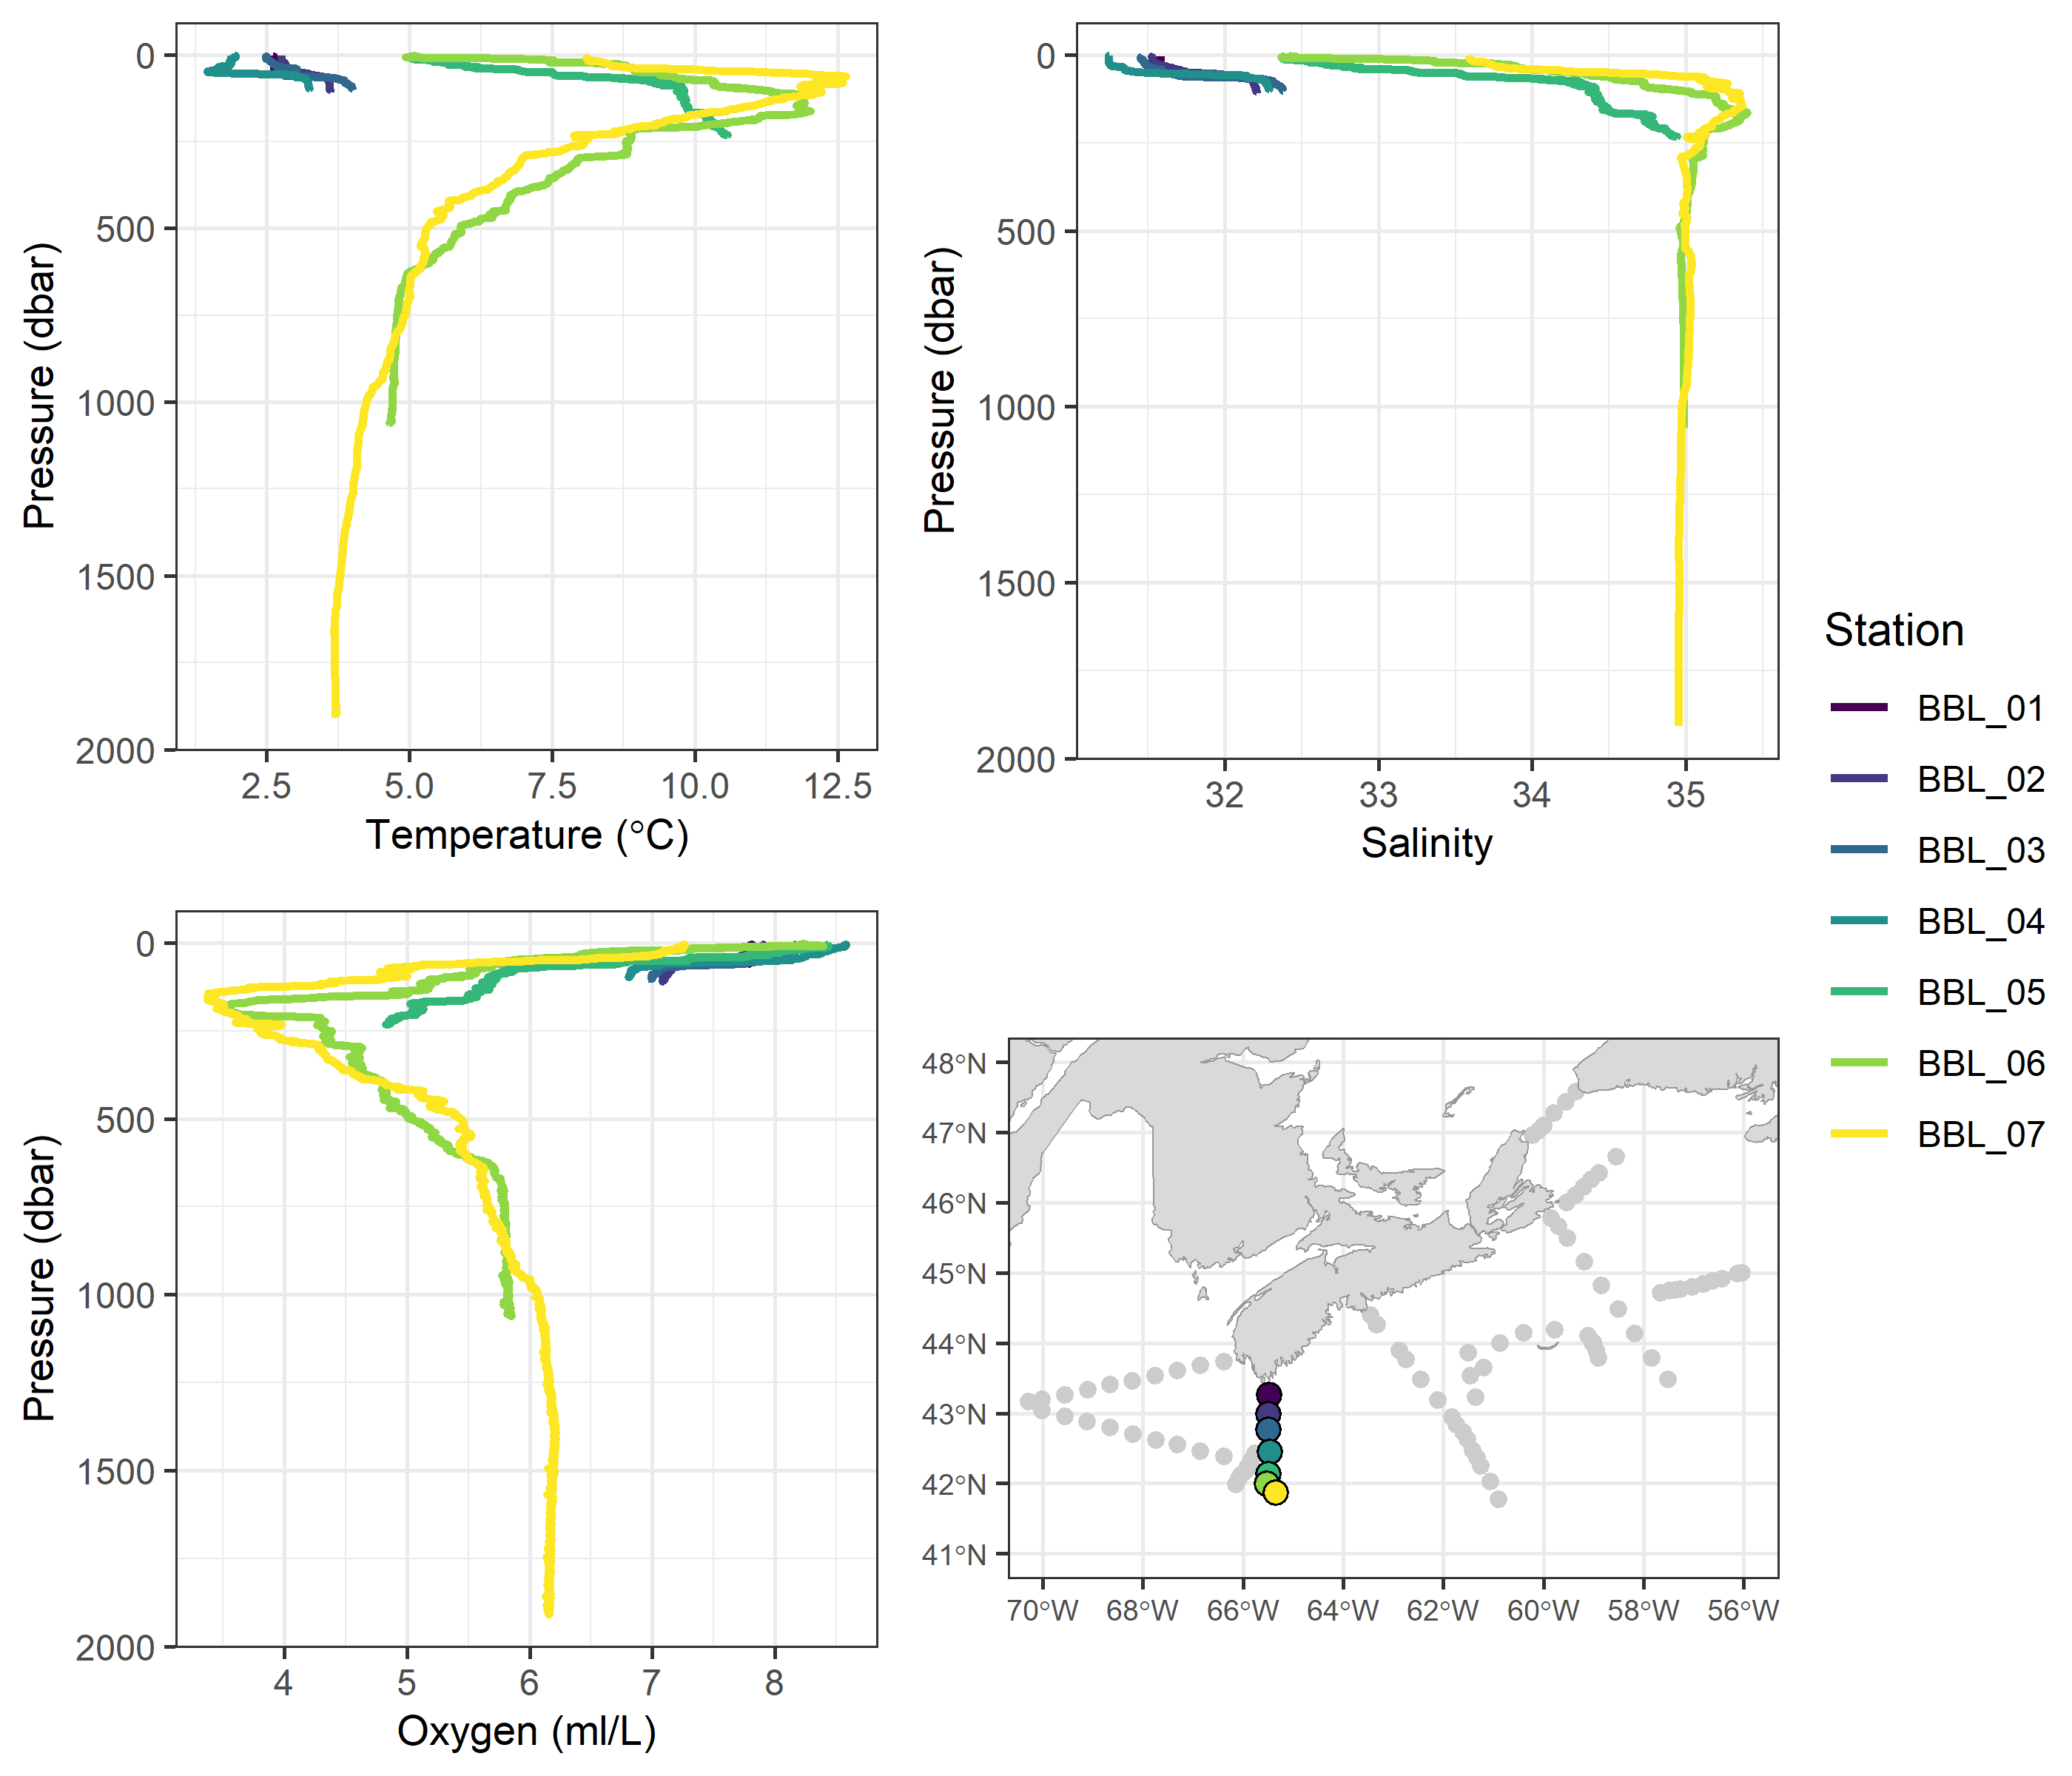
\includegraphics[width=1\linewidth]{figs/EN728_Browns Bank Line_VerticalProfiles}}{Figure} 

}

\caption{Vertical profiles of temperature (top left), salinity (top right), and dissolved oxygen (bottom left) from stations sampled on the Browns Bank Line (BBL; bottom right) during the 2025 spring AZMP mission (EN728).}\label{fig:figureA1}
\end{figure}
\clearpage
\begin{figure}[htb]

{\centering \pdftooltip{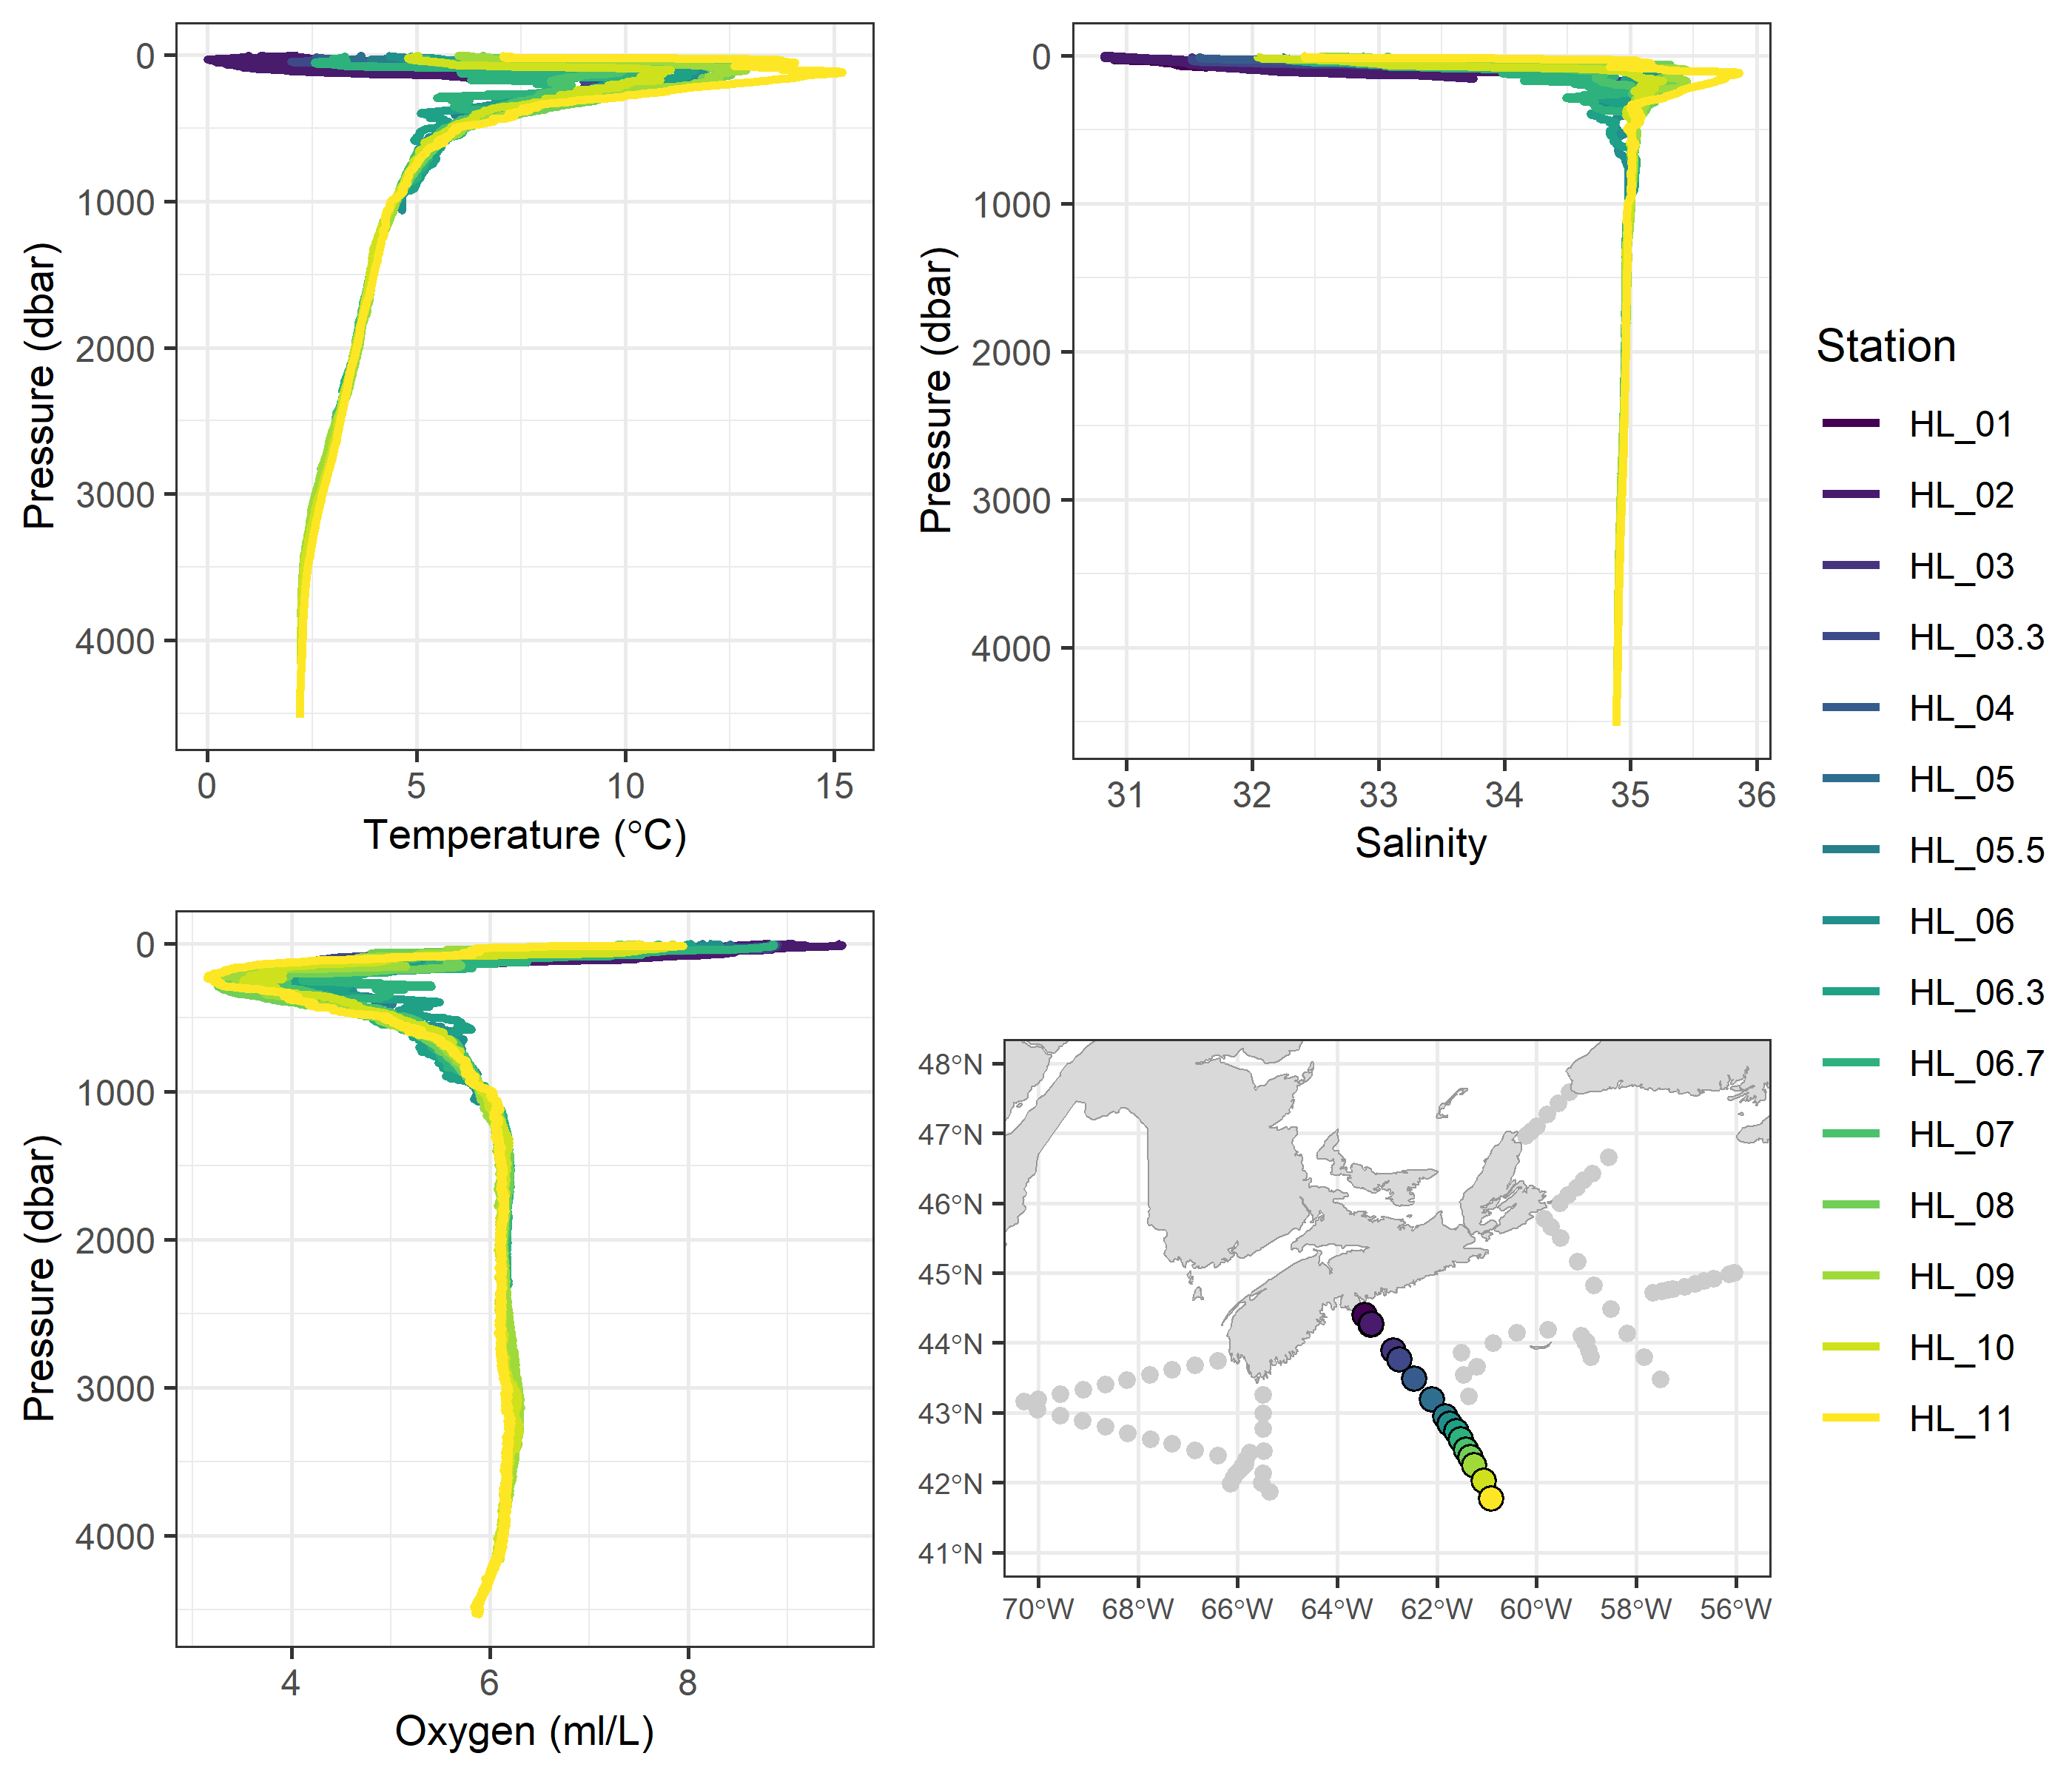
\includegraphics[width=1\linewidth]{figs/EN728_Halifax Line_VerticalProfiles}}{Figure} 

}

\caption{Vertical profiles of temperature (top left), salinity (top right), and dissolved oxygen (bottom left) from stations sampled on the Halifax Line (HL; bottom right) during the 2025 spring AZMP mission (EN728).}\label{fig:figureA2}
\end{figure}
\clearpage
\begin{figure}[htb]

{\centering \pdftooltip{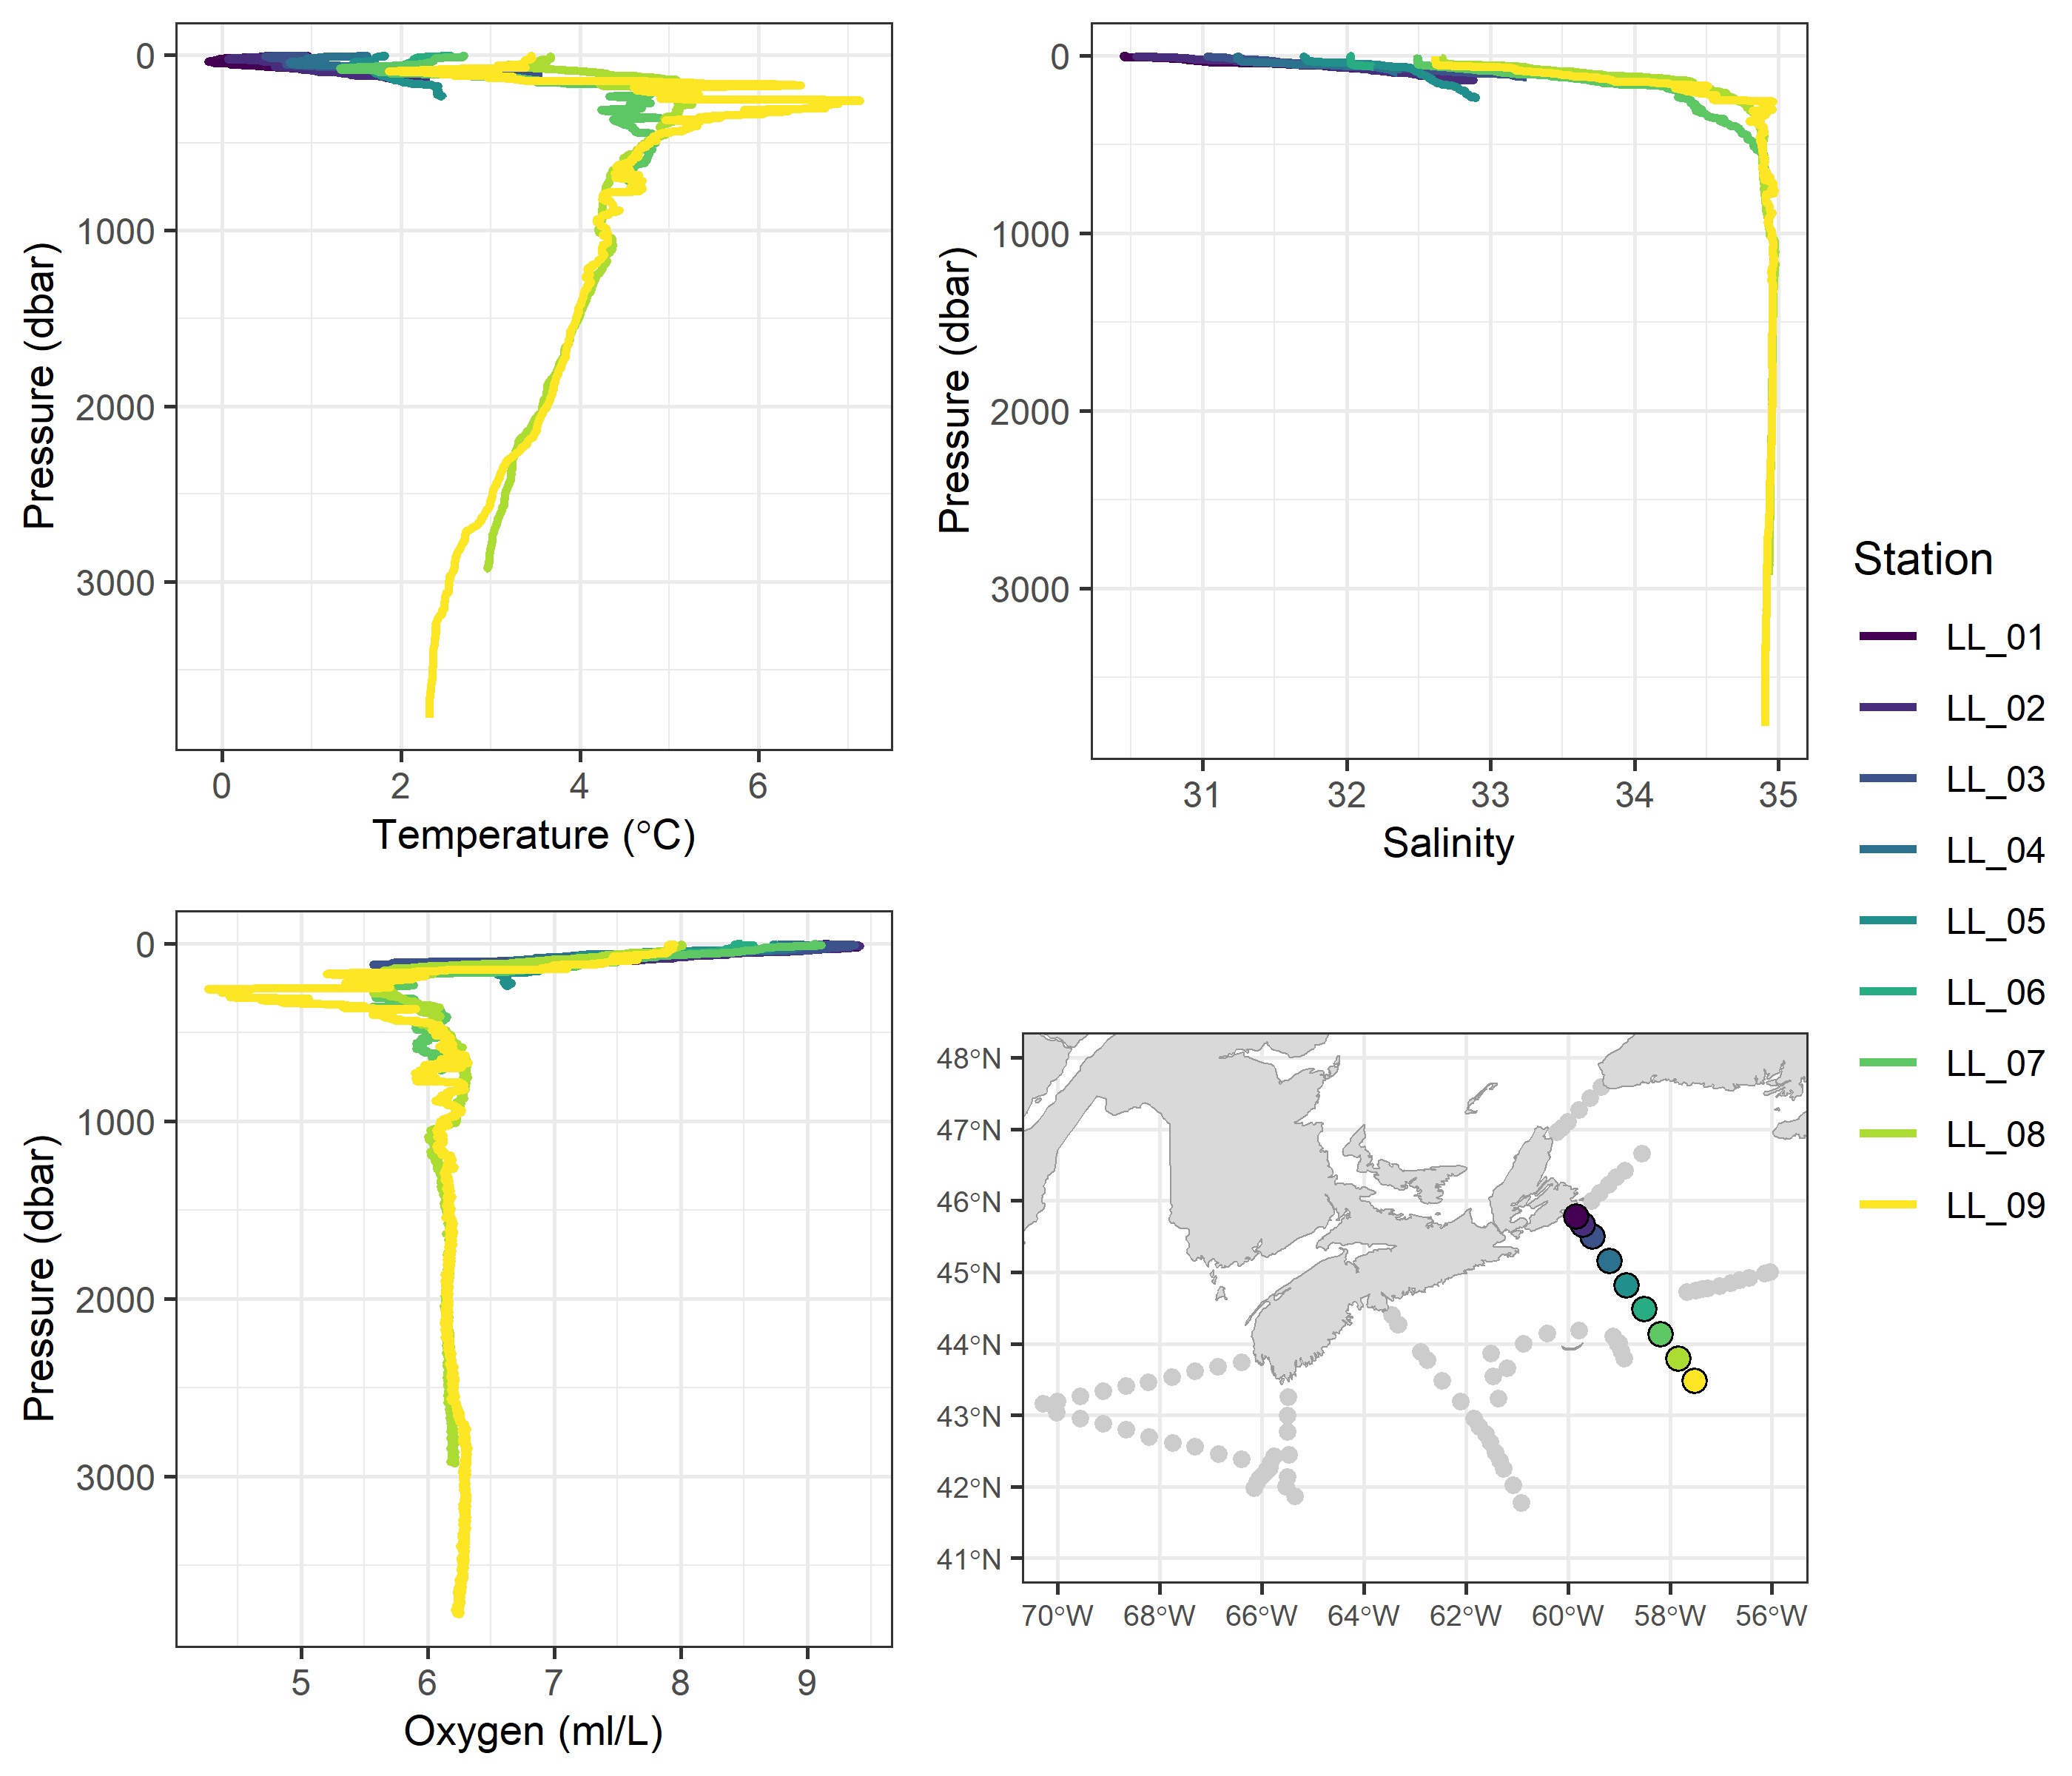
\includegraphics[width=1\linewidth]{figs/EN728_Louisbourg Line_VerticalProfiles}}{Figure} 

}

\caption{Vertical profiles of temperature (top left), salinity (top right), and dissolved oxygen (bottom left) from stations sampled on the Louisbourg Line (LL; bottom right) during the 2025 spring AZMP mission (EN728).}\label{fig:figureA3}
\end{figure}
\clearpage
\begin{figure}[htb]

{\centering \pdftooltip{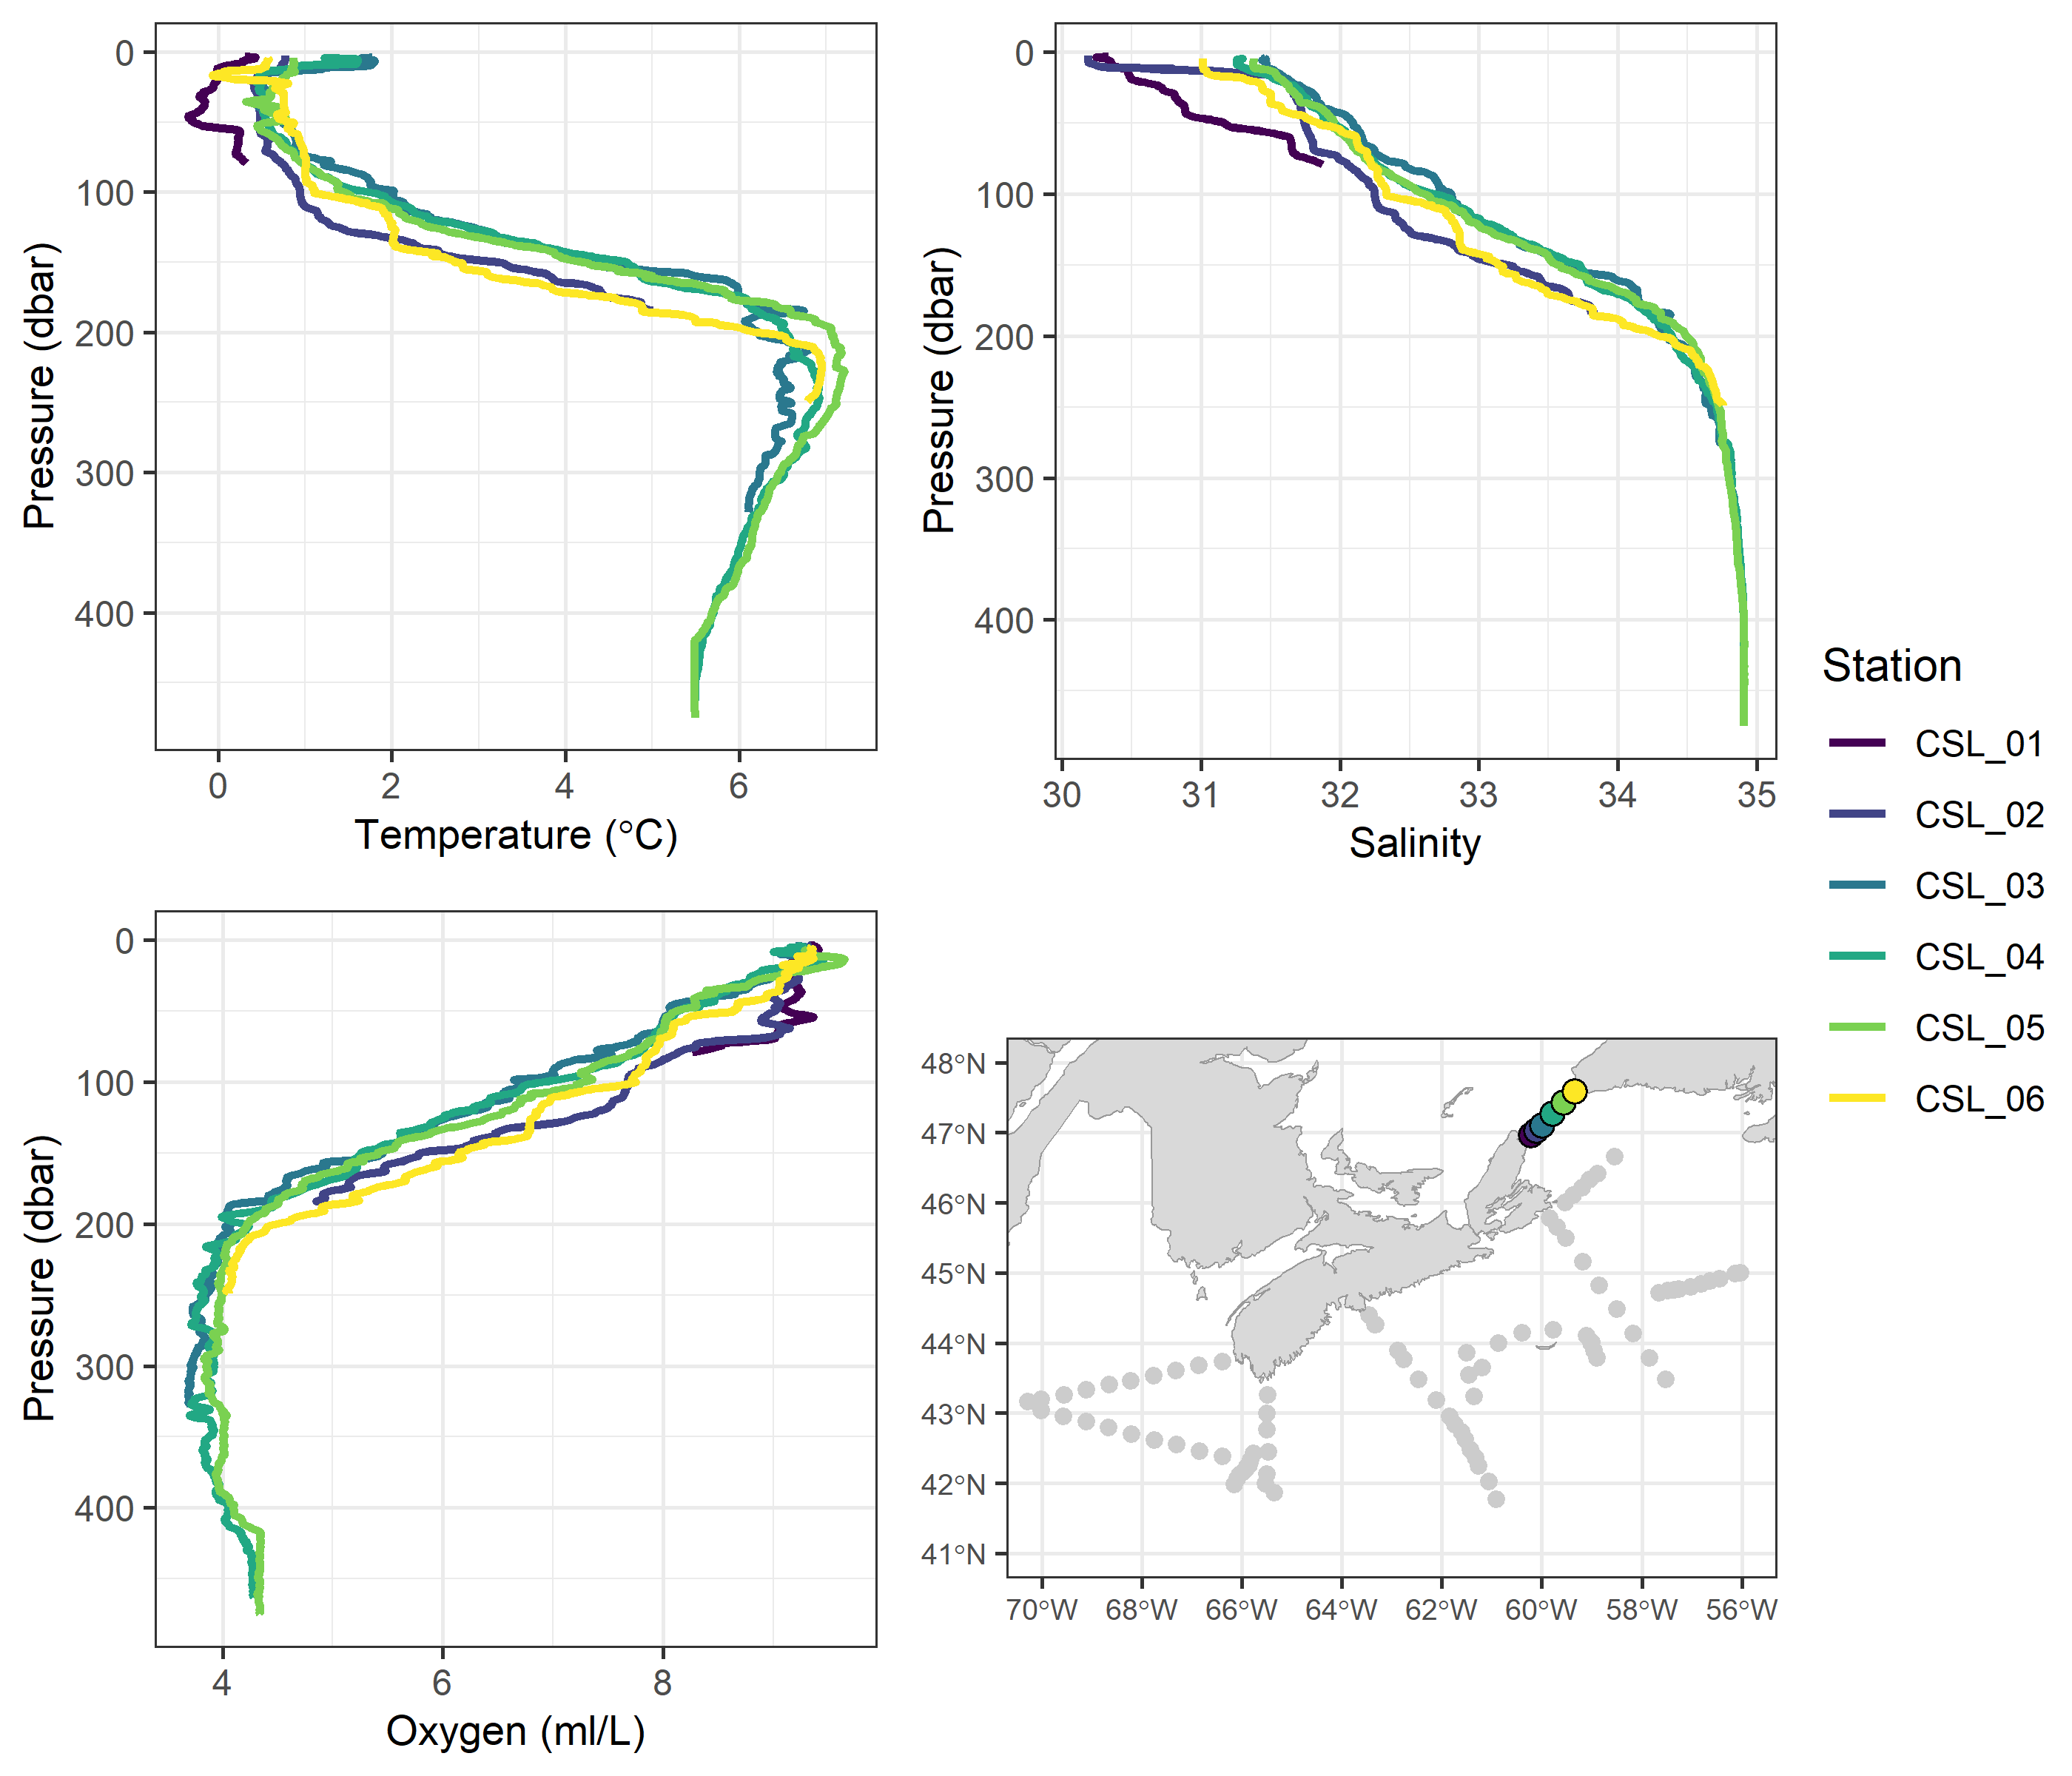
\includegraphics[width=1\linewidth]{figs/EN728_Cabot Strait Line_VerticalProfiles}}{Figure} 

}

\caption{Vertical profiles of temperature (top left), salinity (top right), and dissolved oxygen (bottom rleft) from stations sampled on the Cabot Strait Line (CSL; bottom right) during the 2025 spring AZMP mission (EN728).}\label{fig:figureA4}
\end{figure}
\clearpage
\begin{figure}[htb]

{\centering \pdftooltip{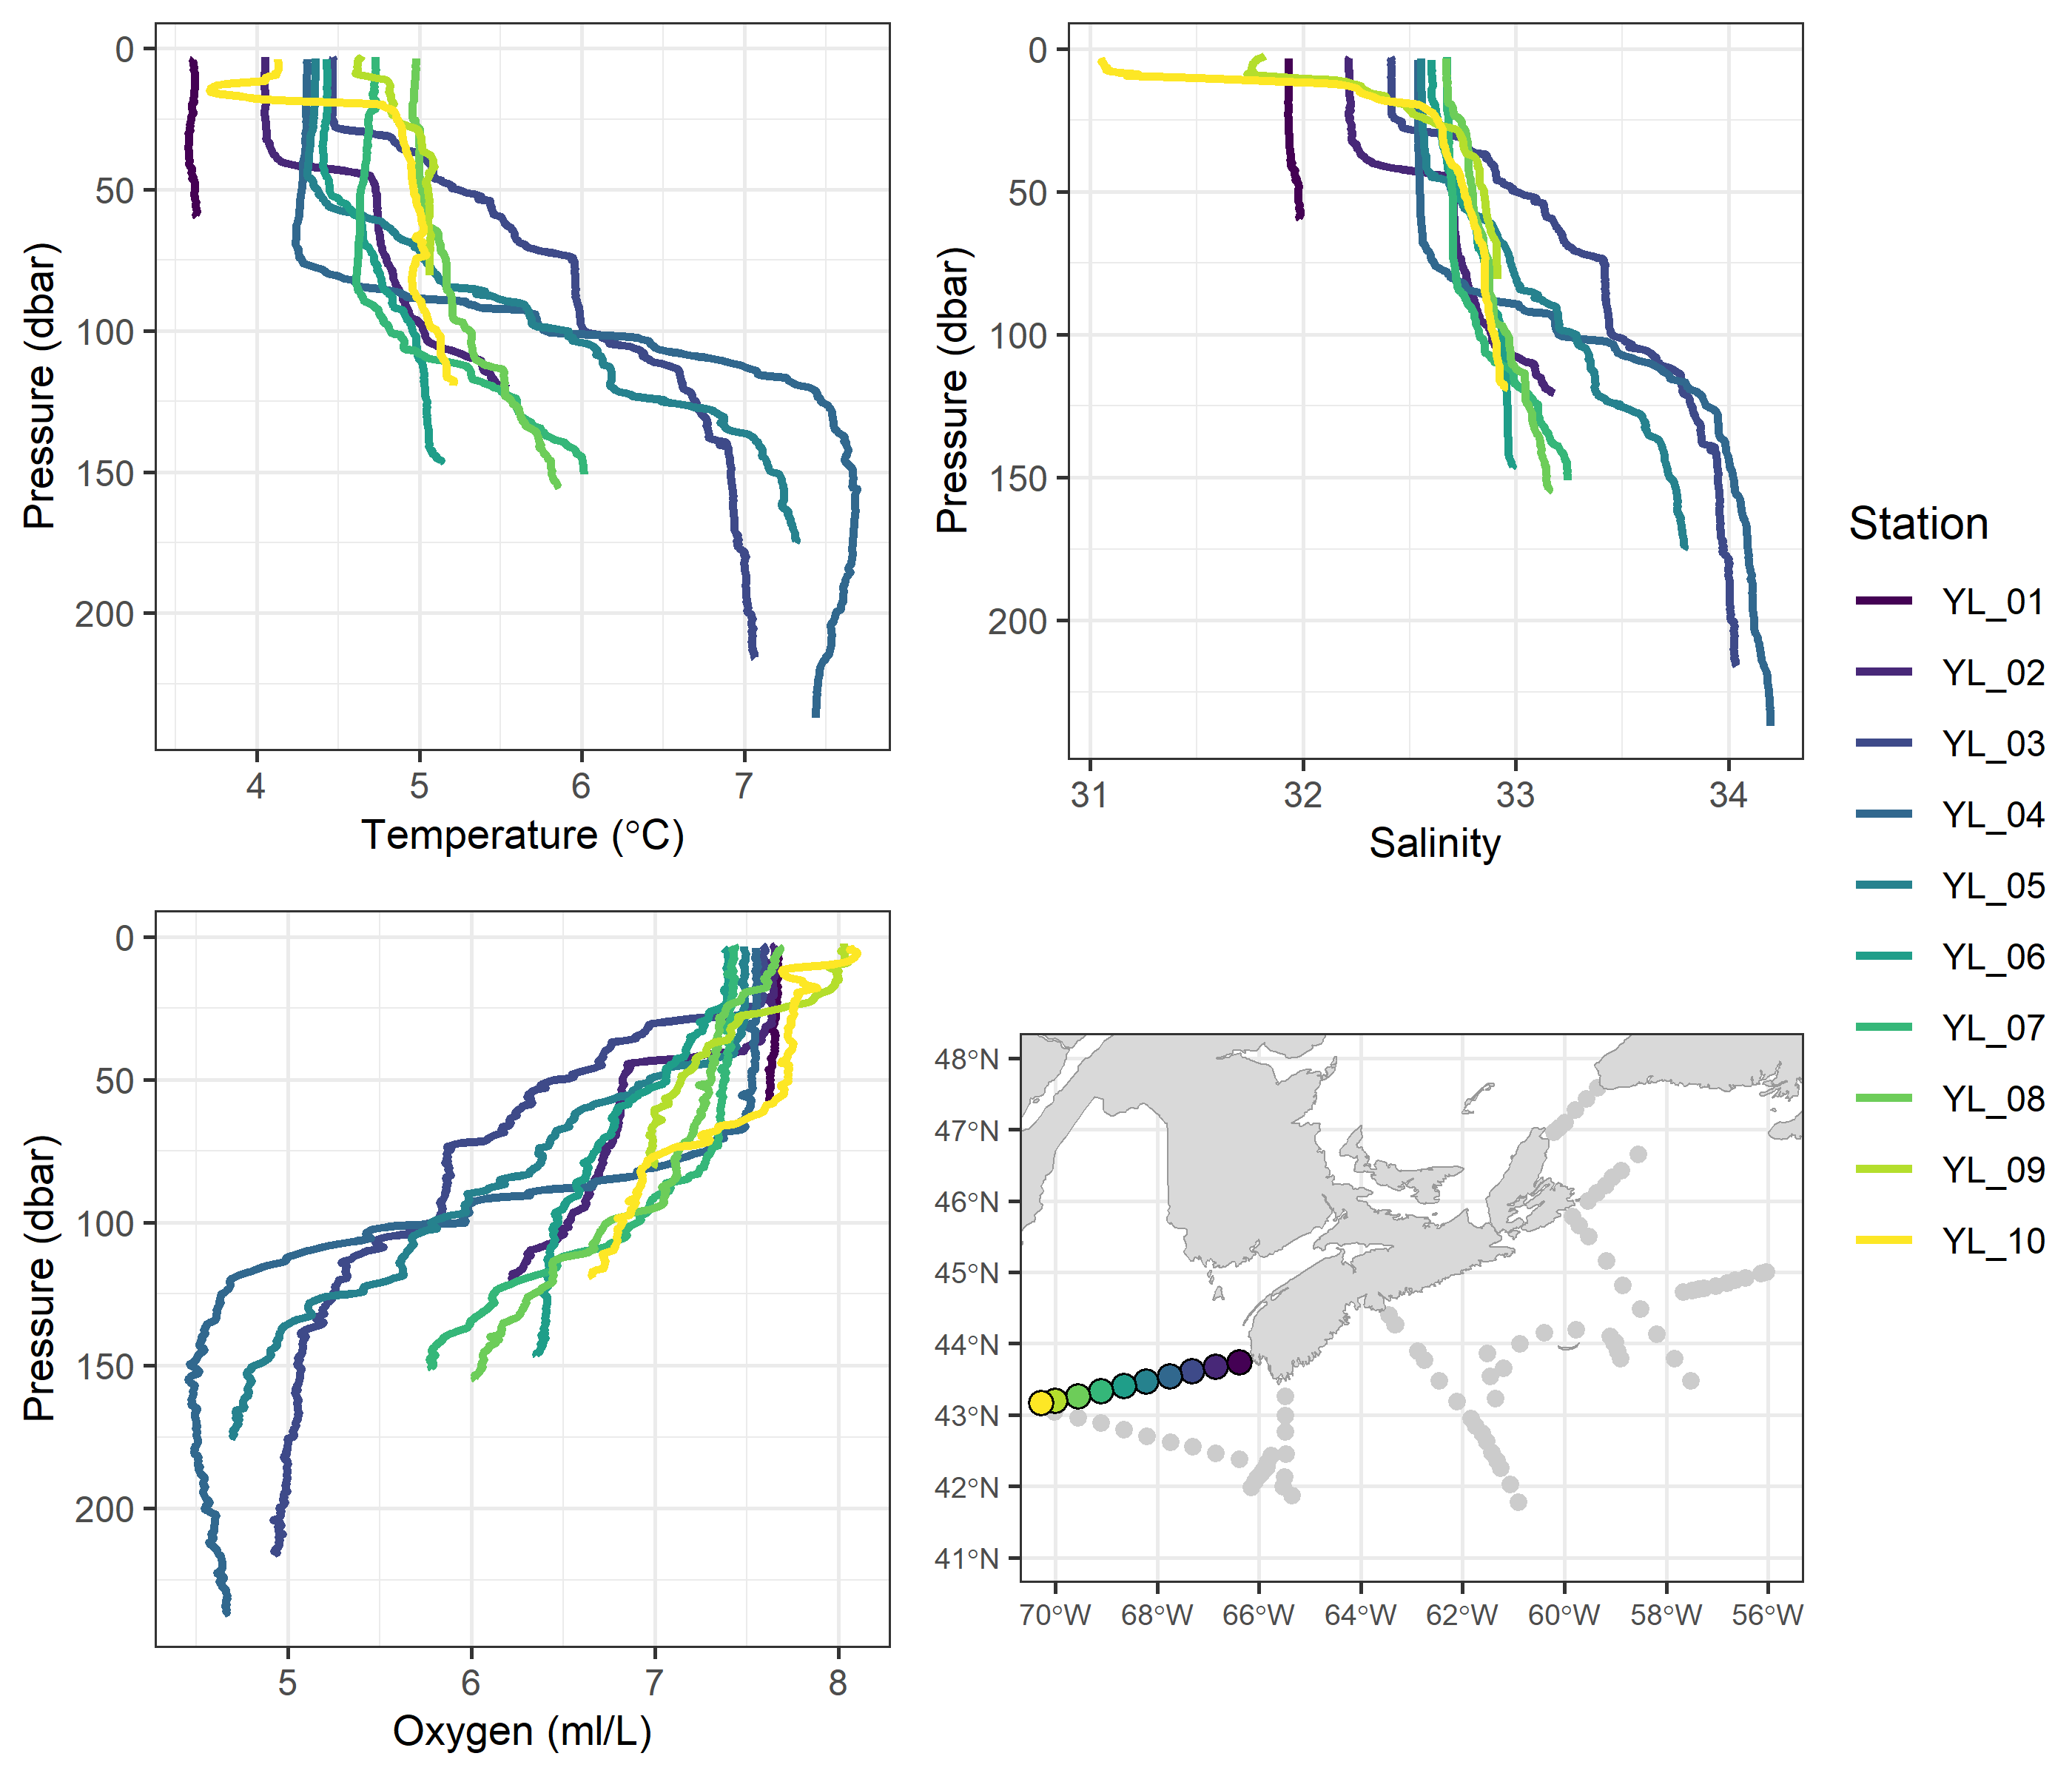
\includegraphics[width=1\linewidth]{figs/EN728_Yarmouth Line_VerticalProfiles}}{Figure} 

}

\caption{Vertical profiles of temperature (top left), salinity (top right), and dissolved oxygen (bottom left) from stations sampled on the Yarmouth Line (YL; bottom right) during the 2025 spring AZMP mission (EN728).}\label{fig:figureA5}
\end{figure}
\clearpage
\begin{figure}[htb]

{\centering \pdftooltip{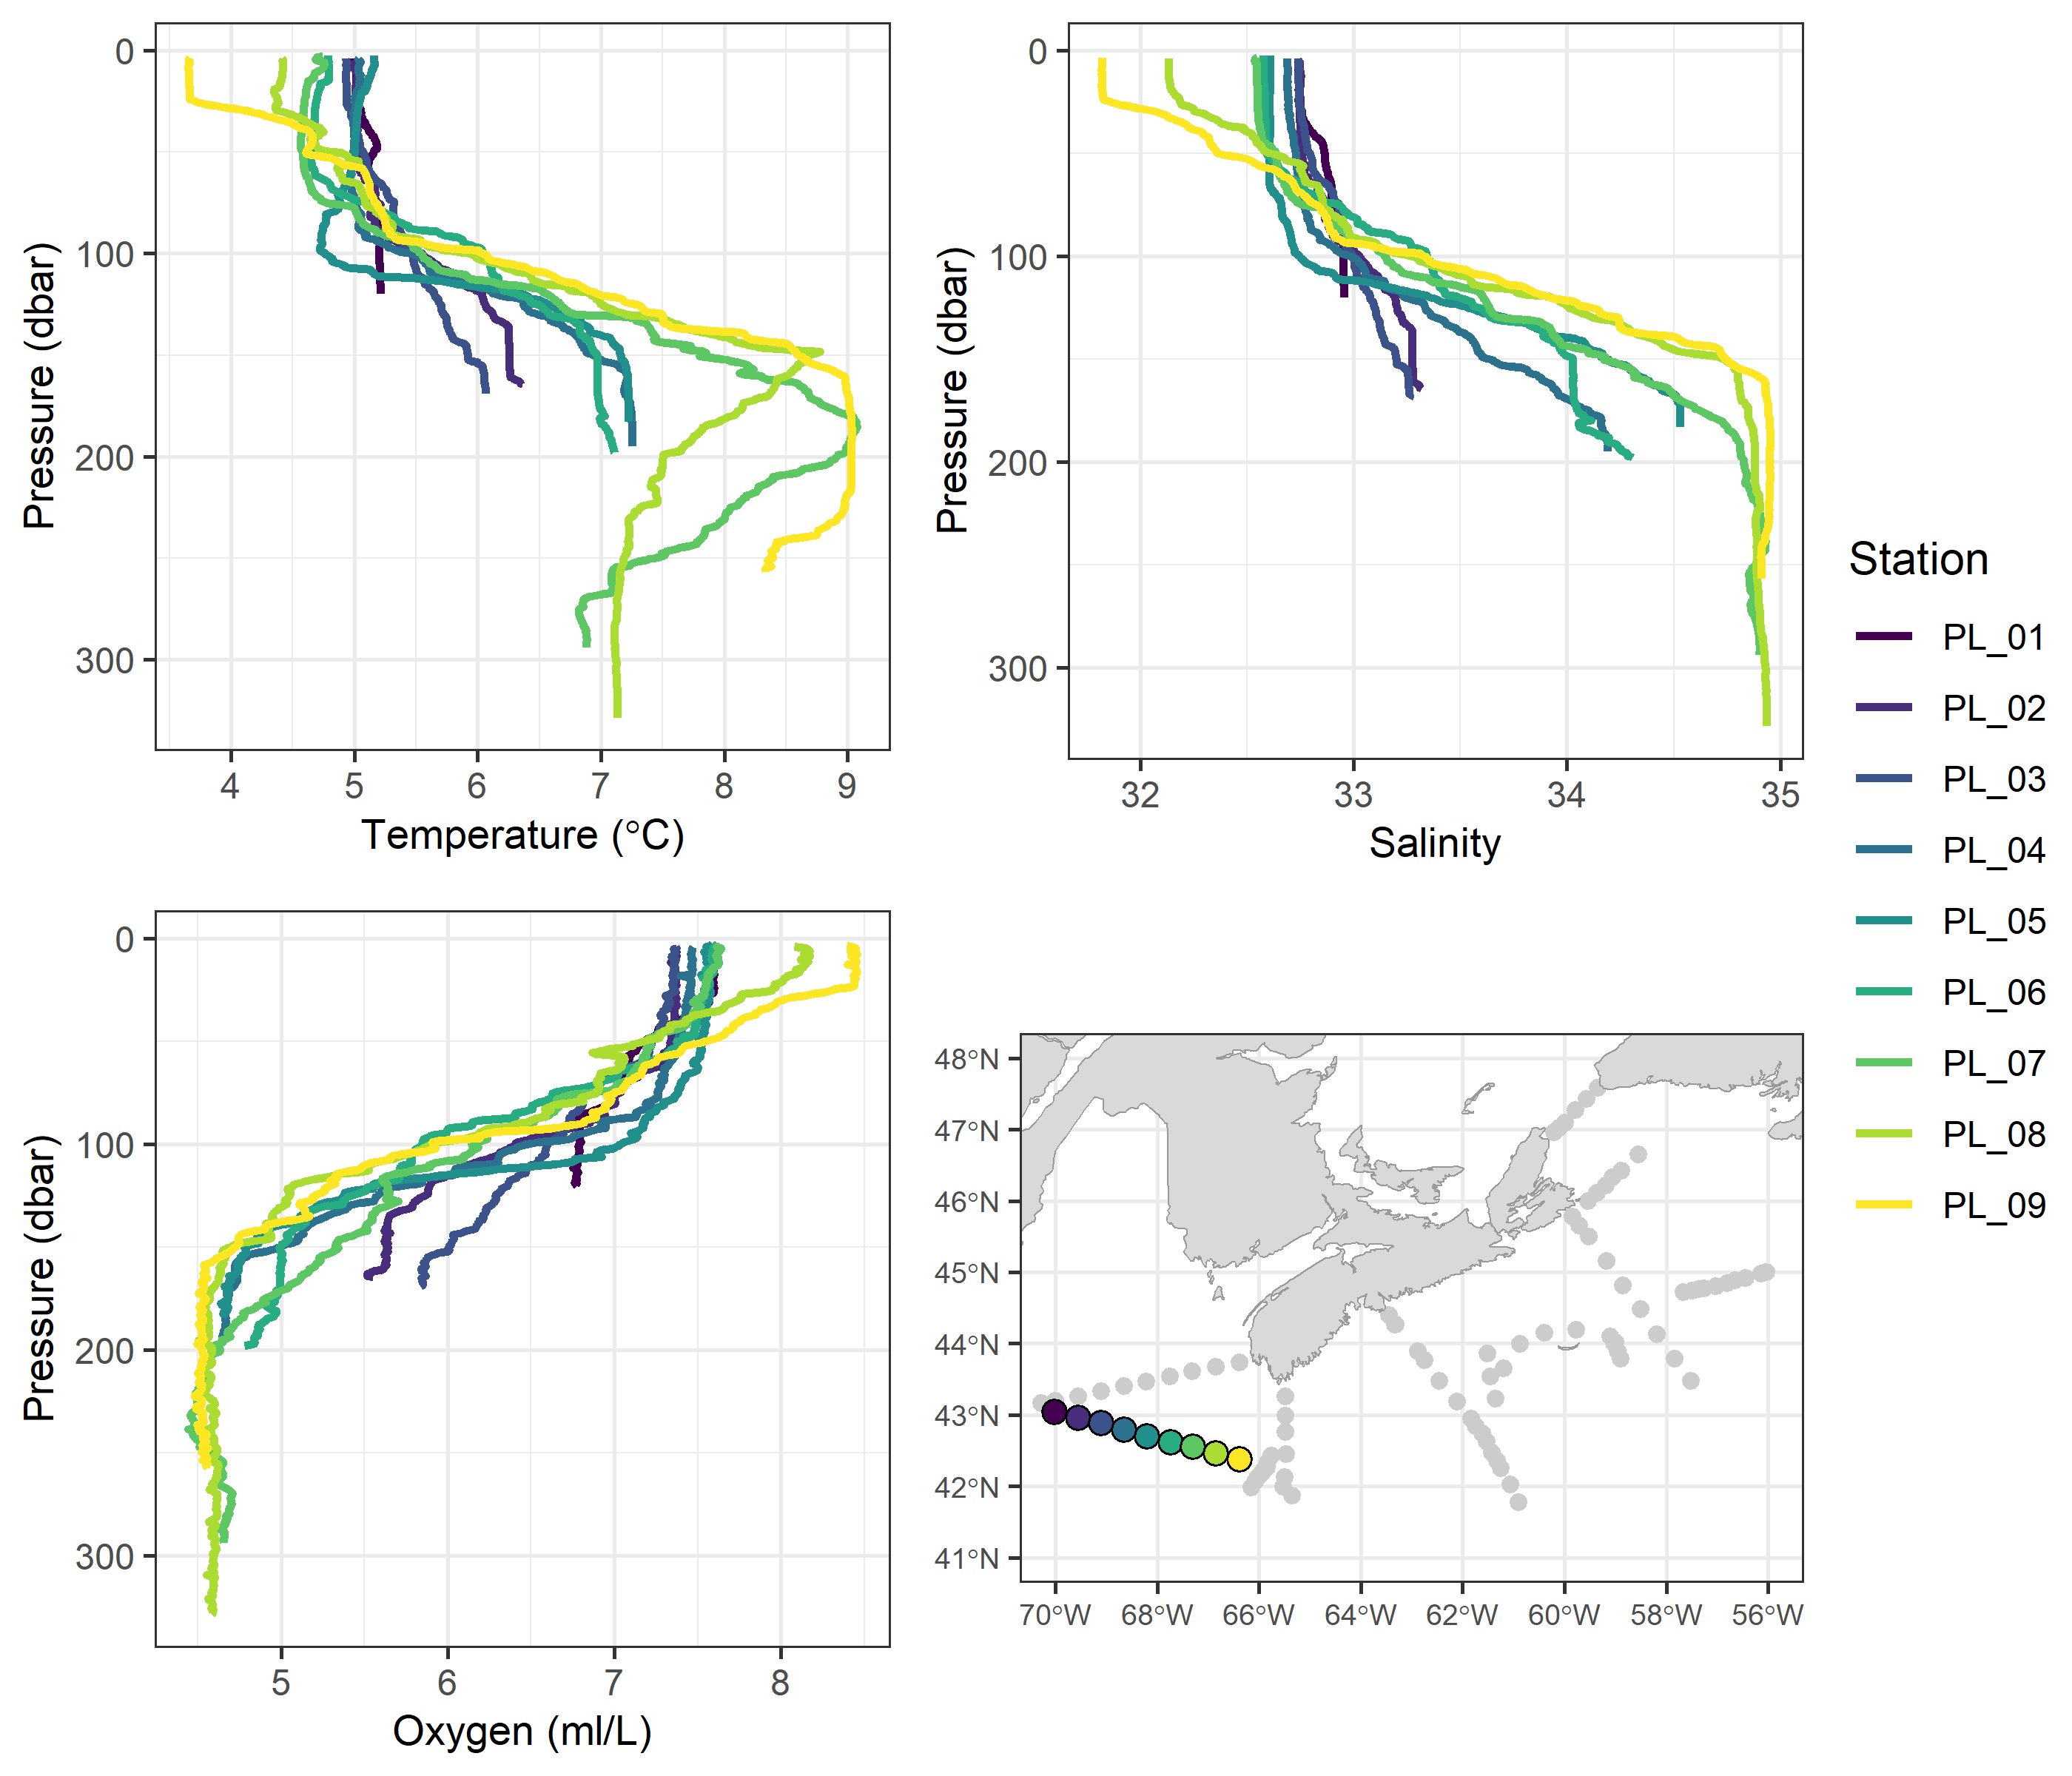
\includegraphics[width=1\linewidth]{figs/EN728_Portsmouth Line_VerticalProfiles}}{Figure} 

}

\caption{Vertical profiles of temperature (top left), salinity (top right), and dissolved oxygen (bottom left) from stations sampled on the Portsmouth Line (PL; bottom right) during the 2025 spring AZMP mission (EN728).}\label{fig:figureA6}
\end{figure}
\clearpage
\begin{figure}[htb]

{\centering \pdftooltip{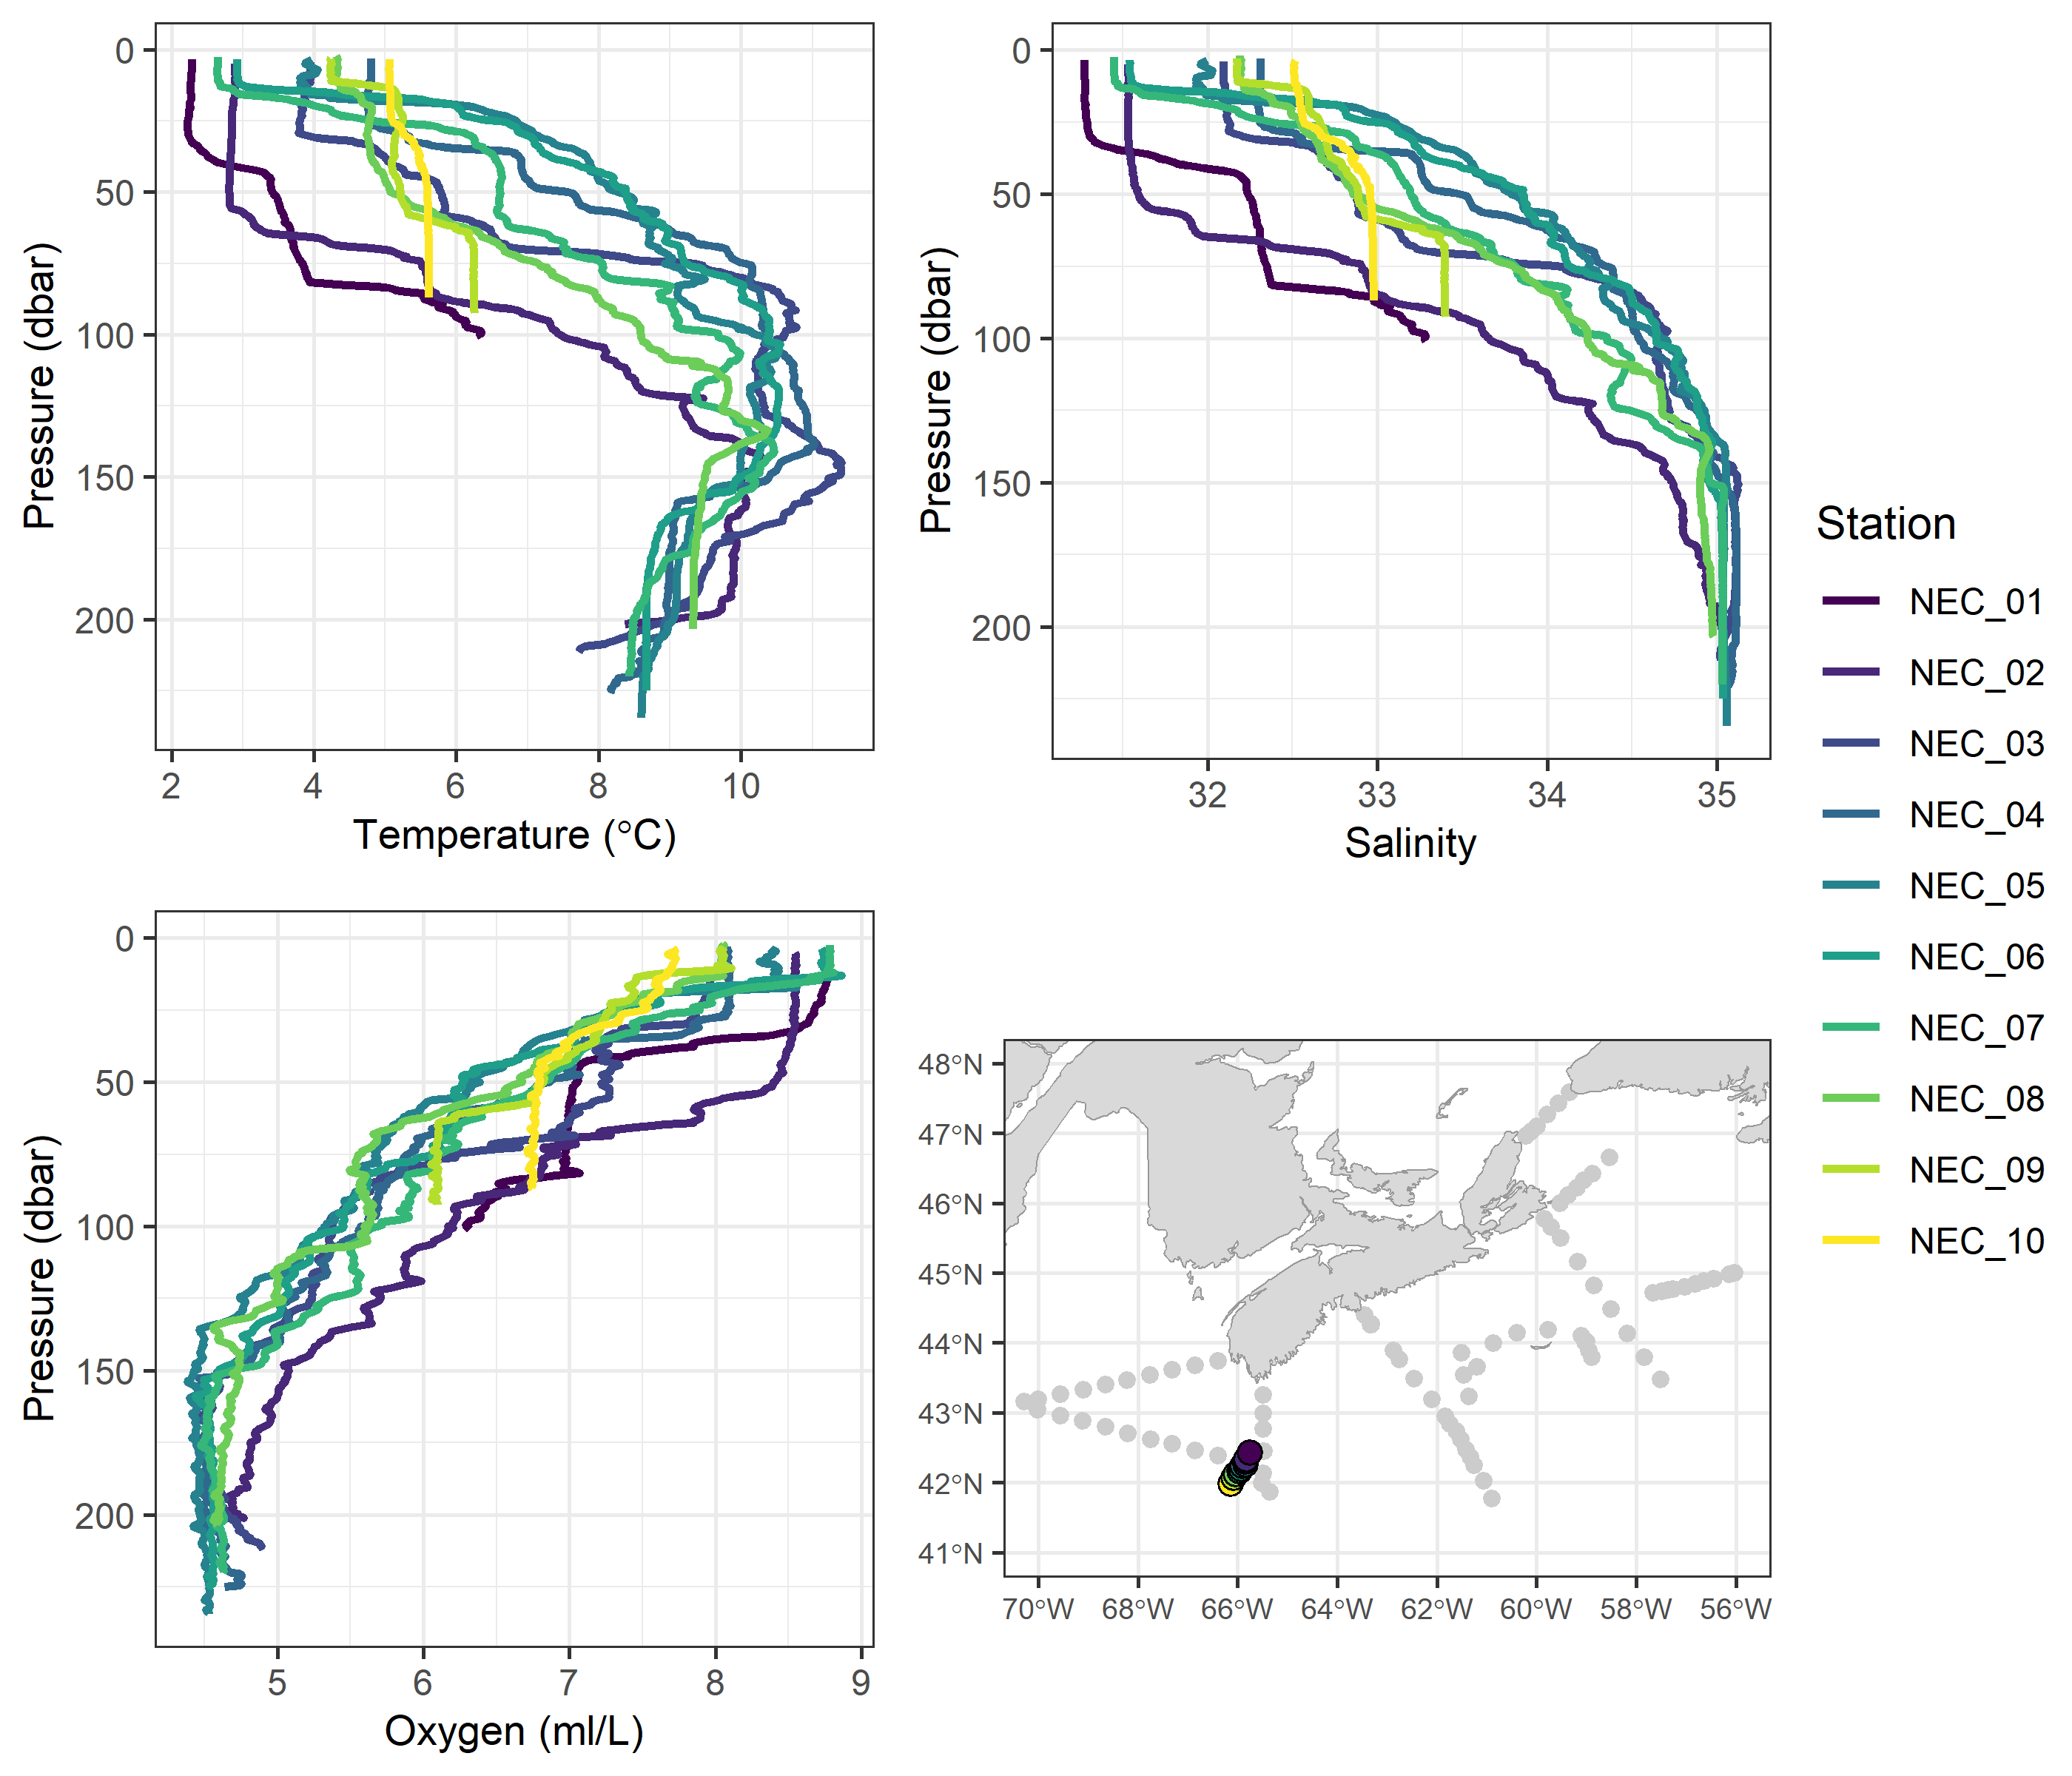
\includegraphics[width=1\linewidth]{figs/EN728_Northeast Channel_VerticalProfiles}}{Figure} 

}

\caption{Vertical profiles of temperature (top left), salinity (top right), and dissolved oxygen (bottom left) from stations sampled in the Northeast Channel (NEC; bottom right) during the 2025 spring AZMP mission (EN728).}\label{fig:figureA7}
\end{figure}
\clearpage
\begin{figure}[htb]

{\centering \pdftooltip{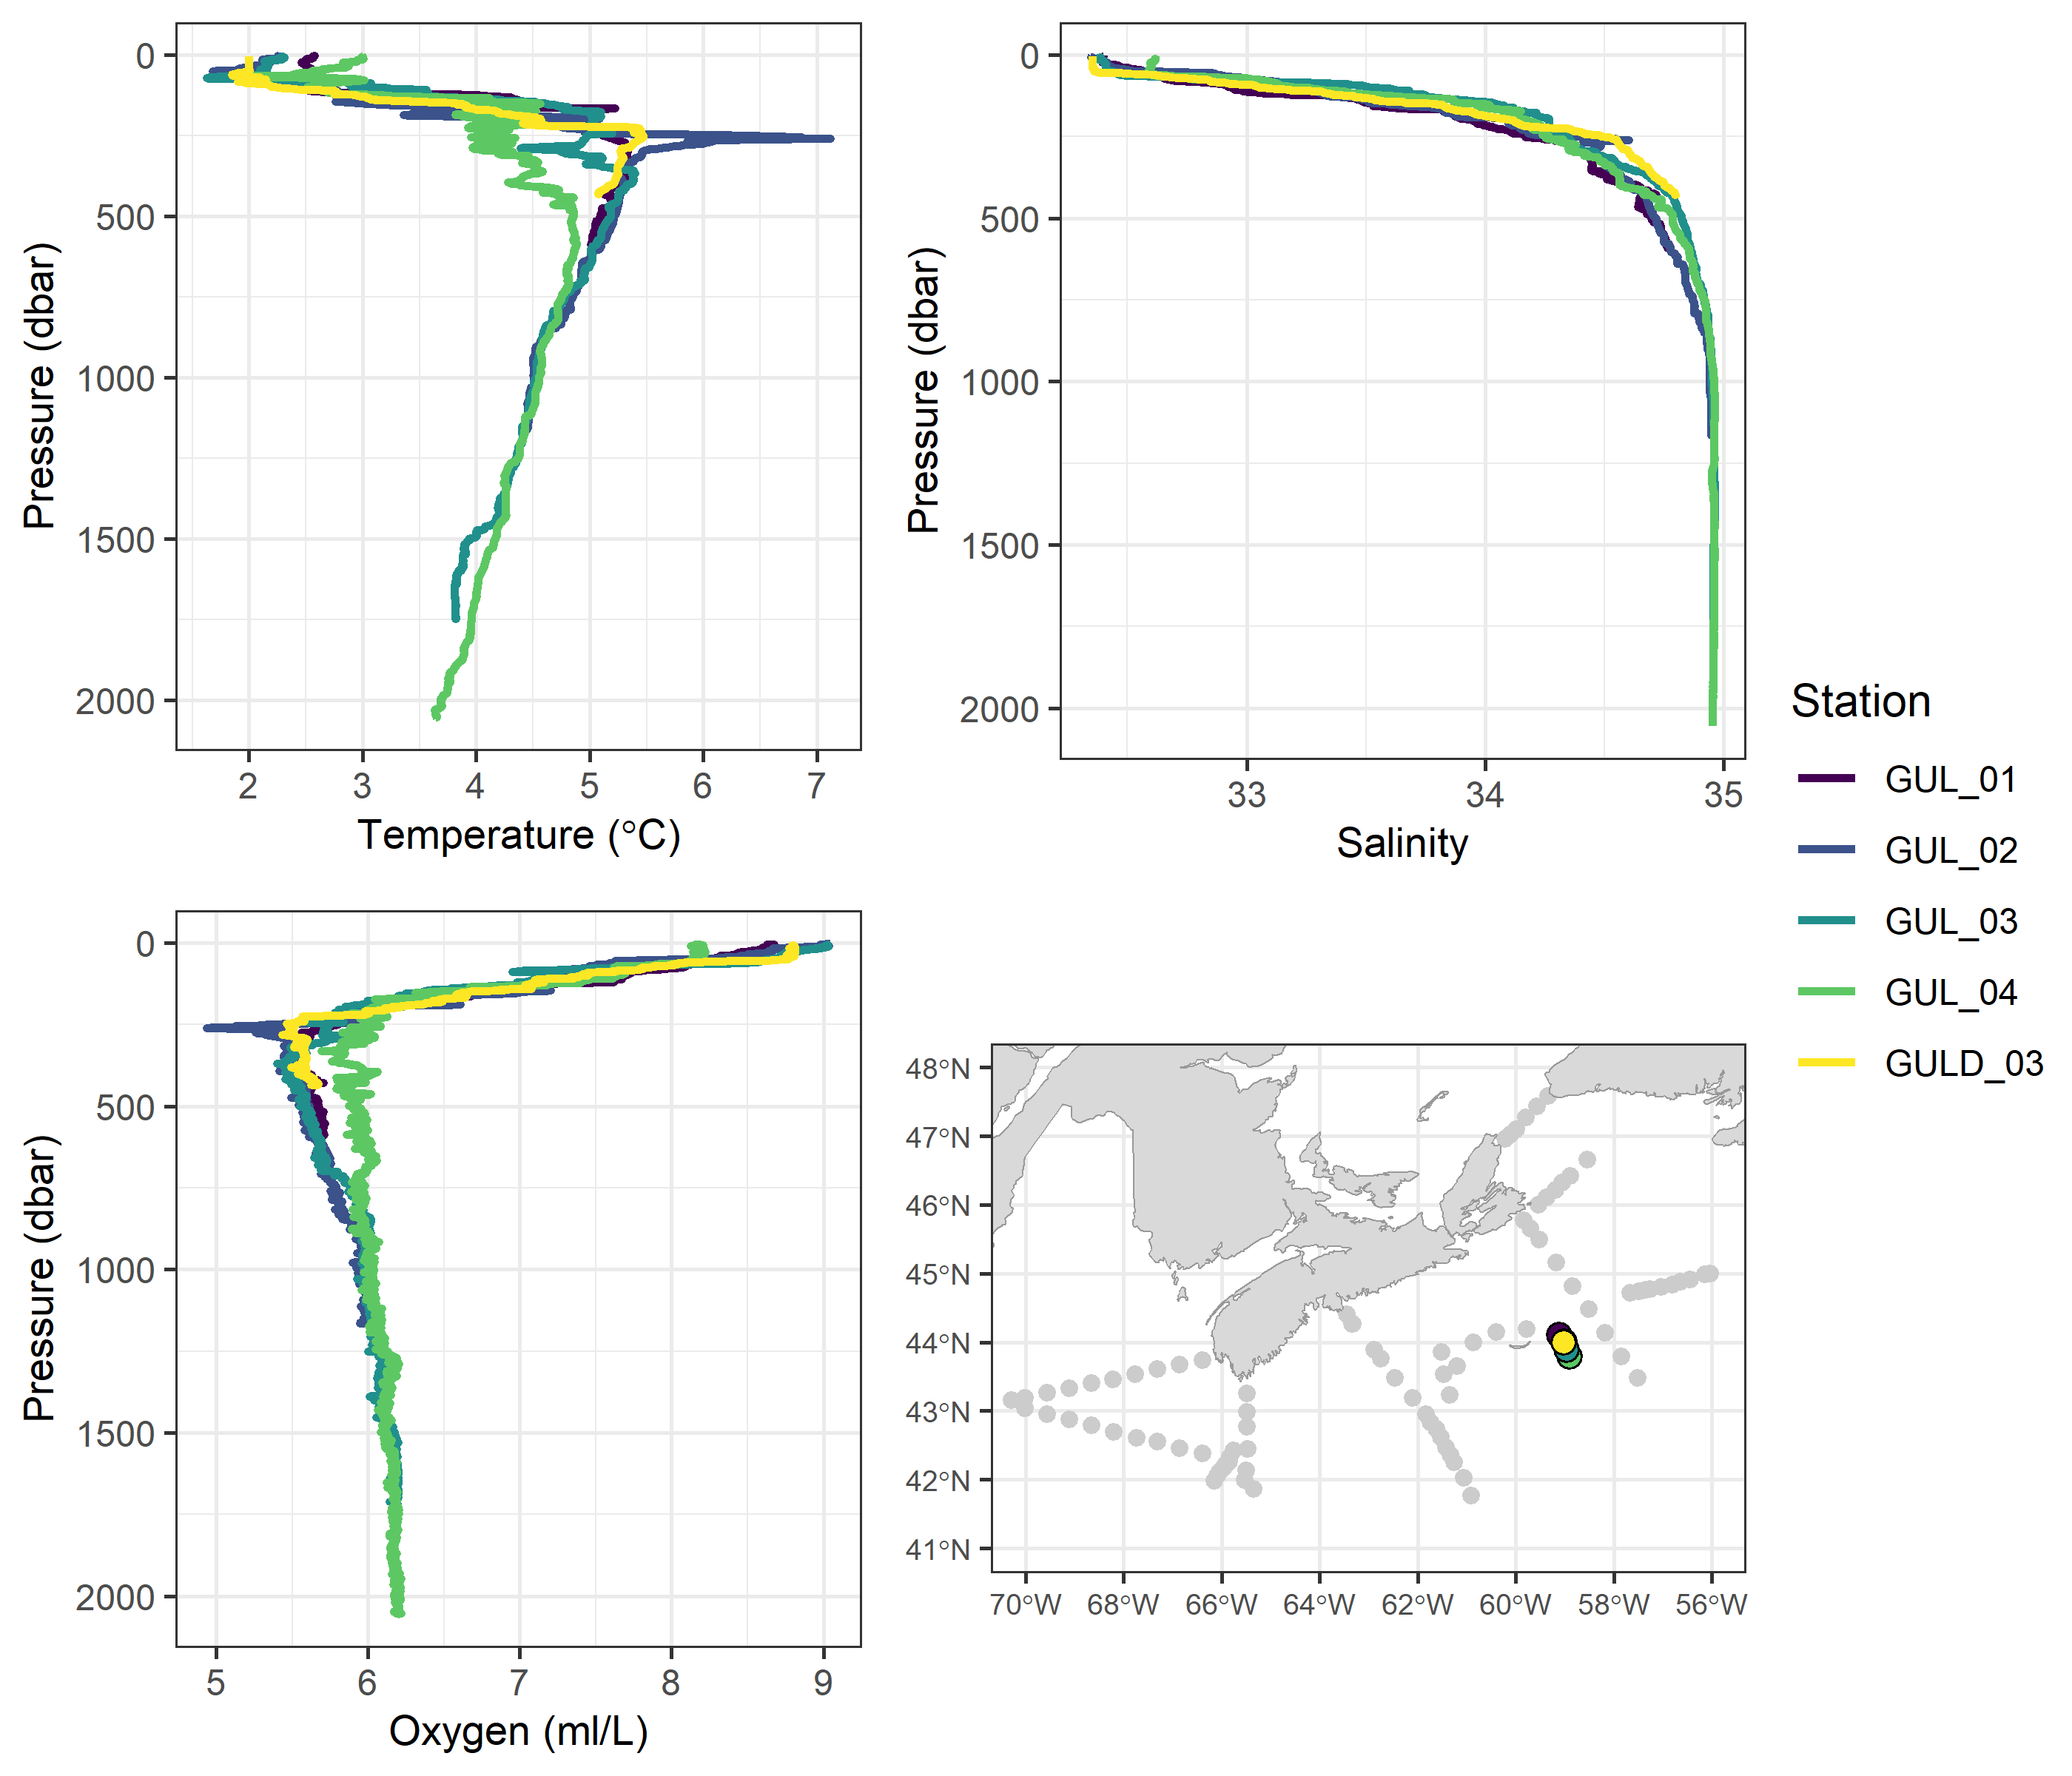
\includegraphics[width=1\linewidth]{figs/EN728_Gully_VerticalProfiles}}{Figure} 

}

\caption{Vertical profiles of temperature (top left), salinity (top right), and dissolved oxygen (bottom left) from stations sampled in the Gully (GUL; bottom right) during the 2025 spring AZMP mission (EN728).}\label{fig:figureA8}
\end{figure}
\clearpage
\begin{figure}[htb]

{\centering \pdftooltip{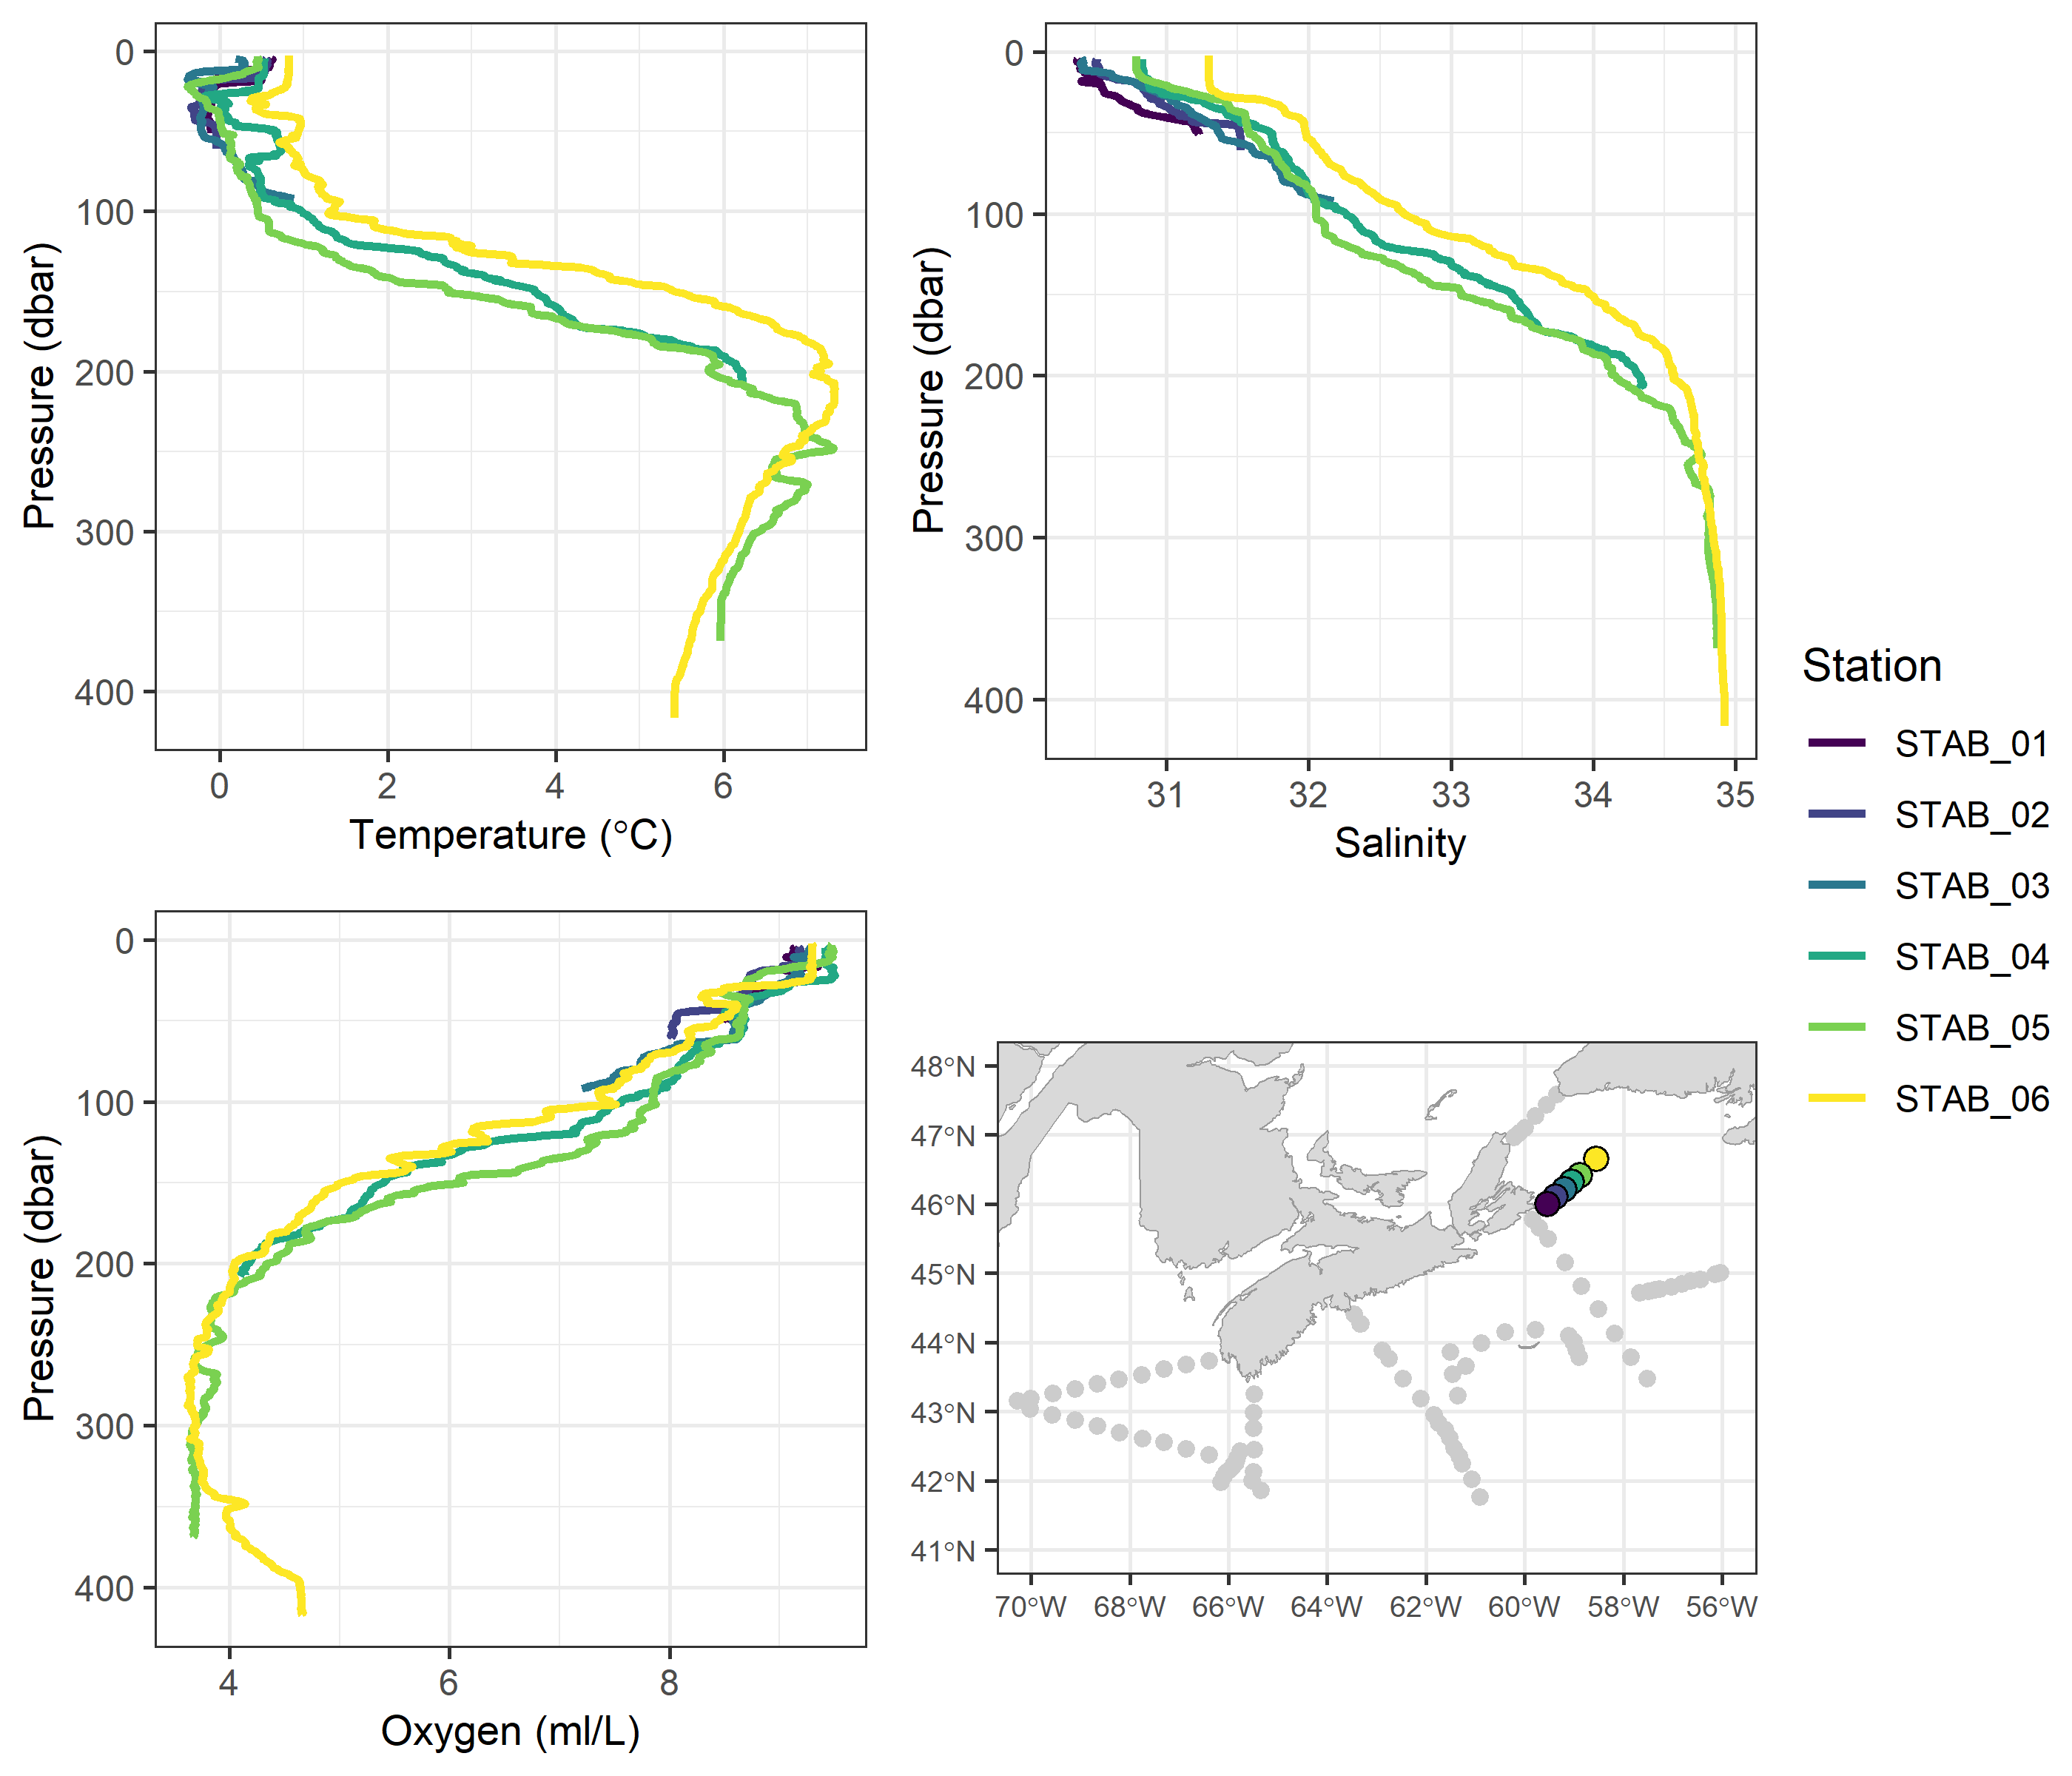
\includegraphics[width=1\linewidth]{figs/EN728_St. Anns Bank_VerticalProfiles}}{Figure} 

}

\caption{Vertical profiles of temperature (top left), salinity (top right), and dissolved oxygen (bottom left) from stations sampled on St. Anns Bank (STAB; bottom right) during the 2025 spring AZMP mission (EN728).}\label{fig:figureA9}
\end{figure}
\clearpage
\begin{figure}[htb]

{\centering \pdftooltip{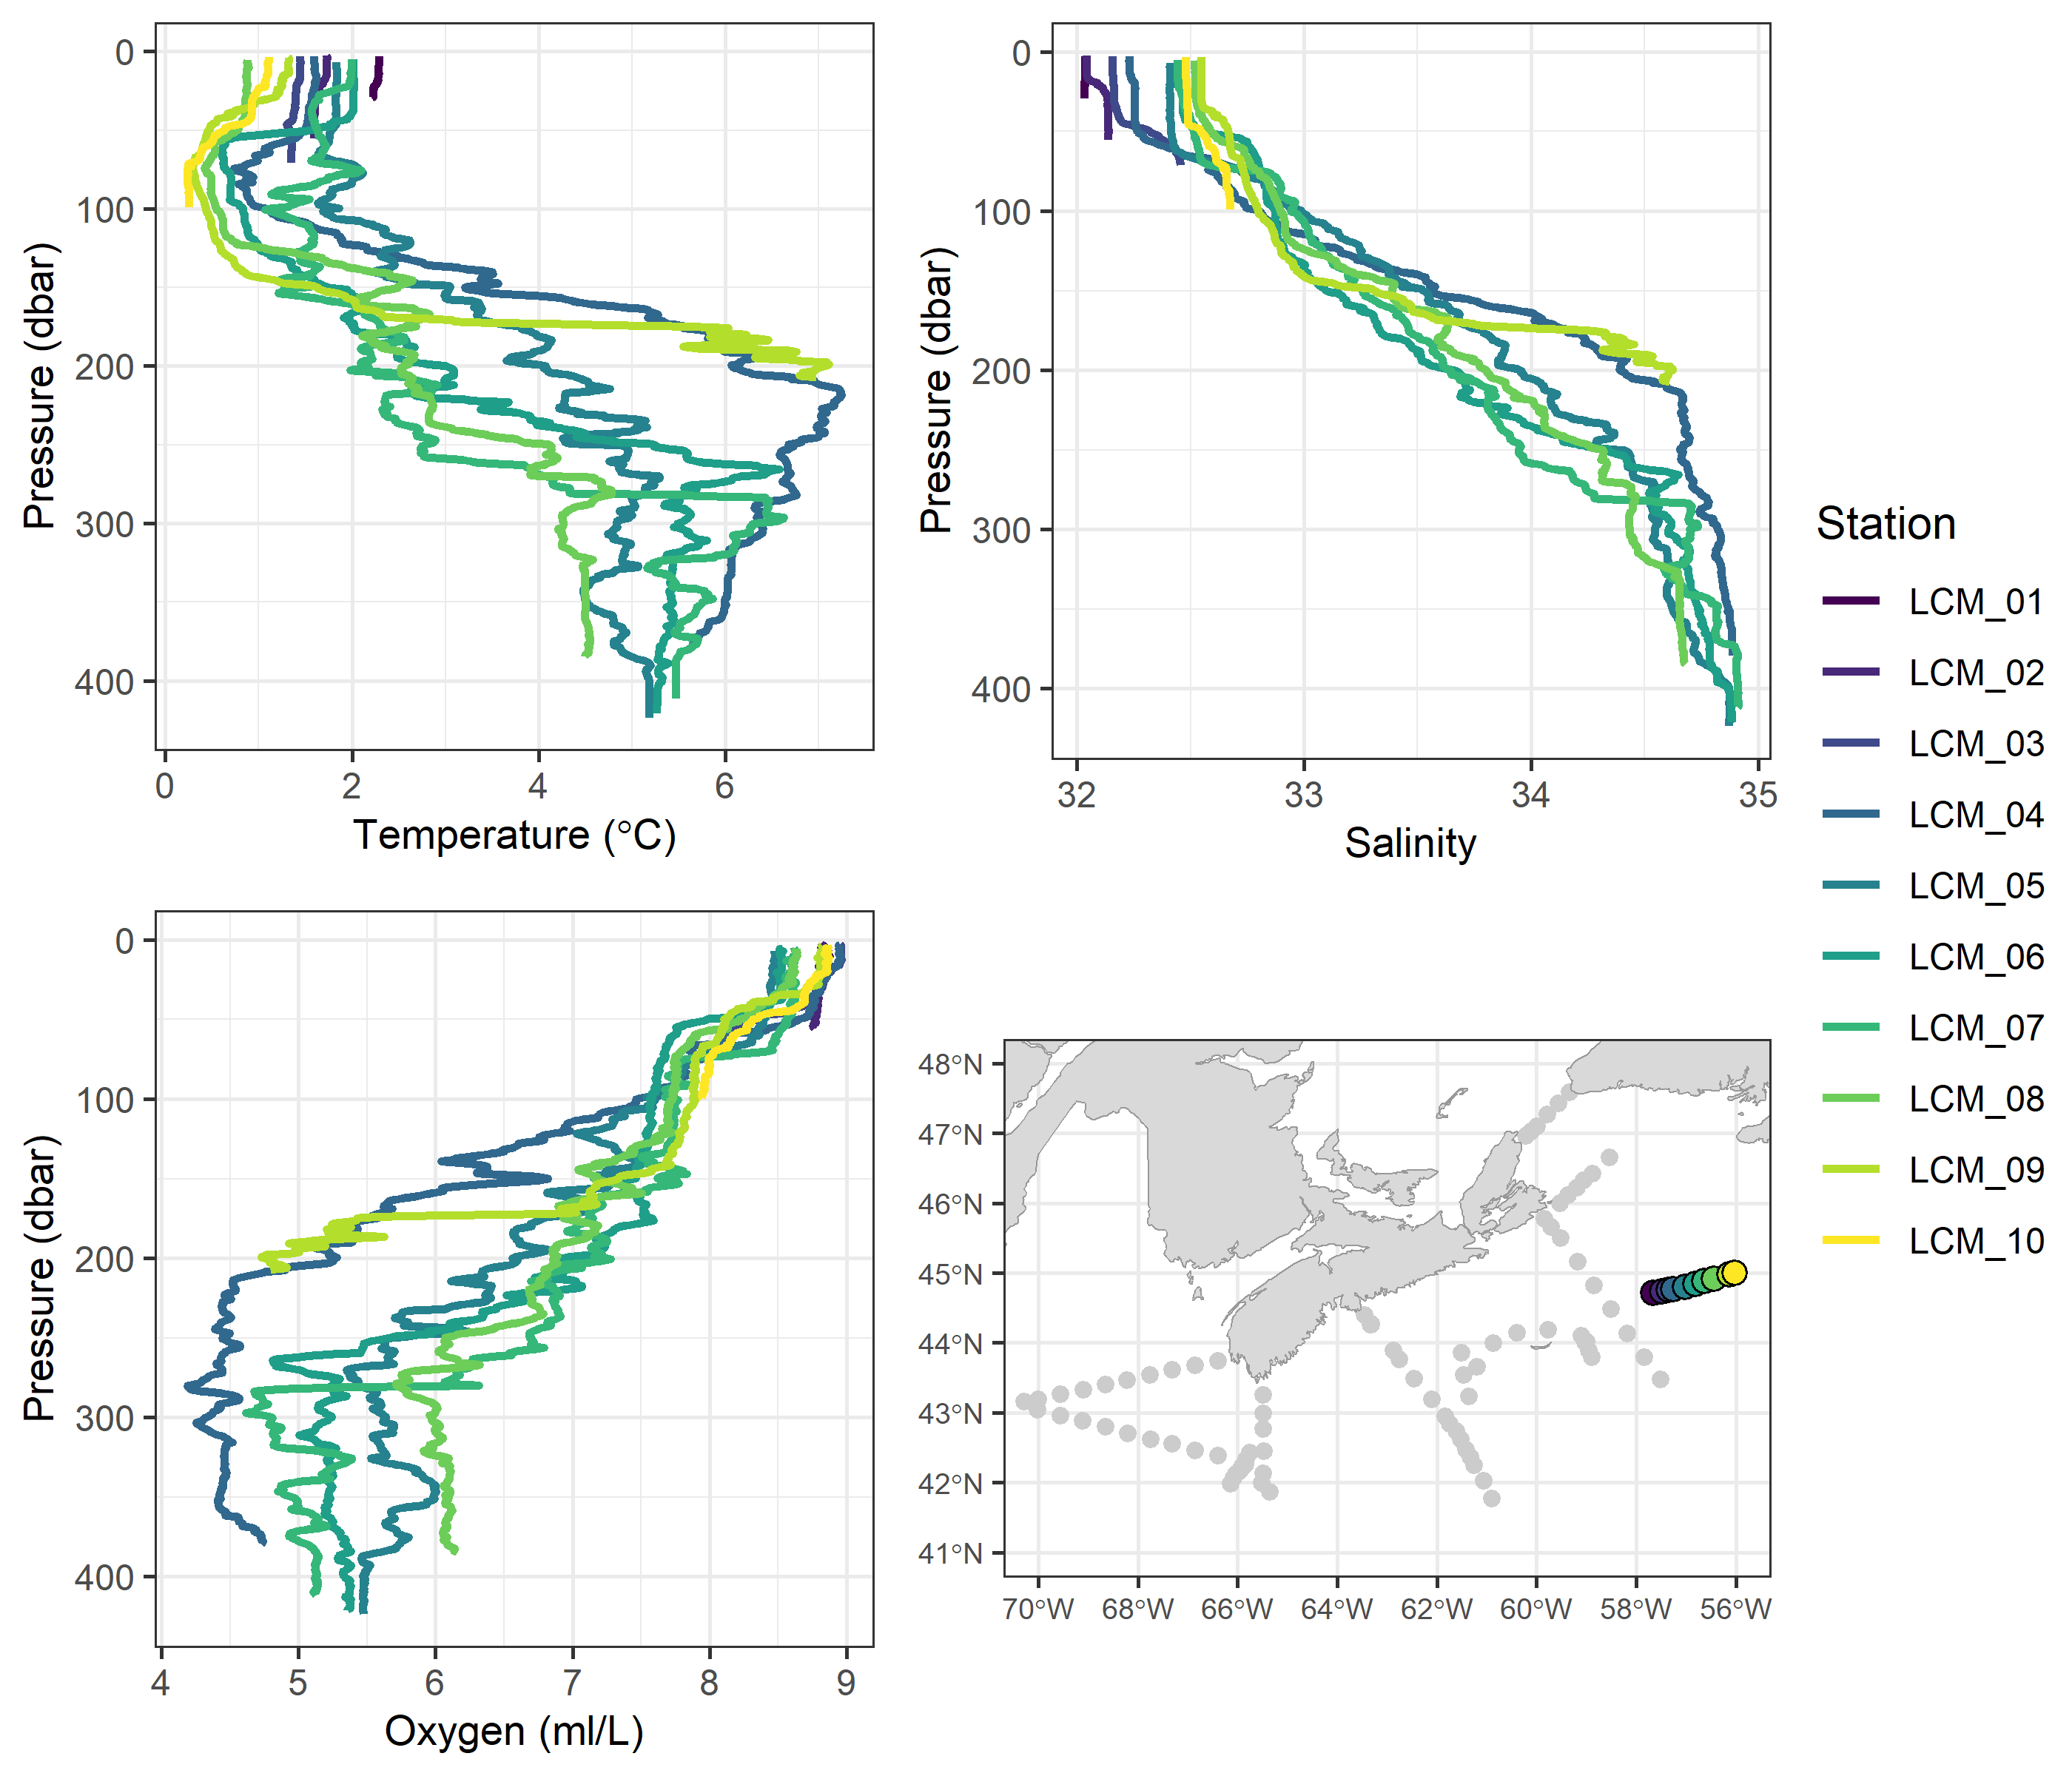
\includegraphics[width=1\linewidth]{figs/EN728_Laurentian Channel Mouth_VerticalProfiles}}{Figure} 

}

\caption{Vertical profiles of temperature (top left), salinity (top right), and dissolved oxygen (bottom left) from stations sampled in the Laurentian Channel Mouth (LCM; bottom right) during the 2025 spring AZMP mission (EN728).}\label{fig:figureA10}
\end{figure}
\clearpage
\begin{figure}[htb]

{\centering \pdftooltip{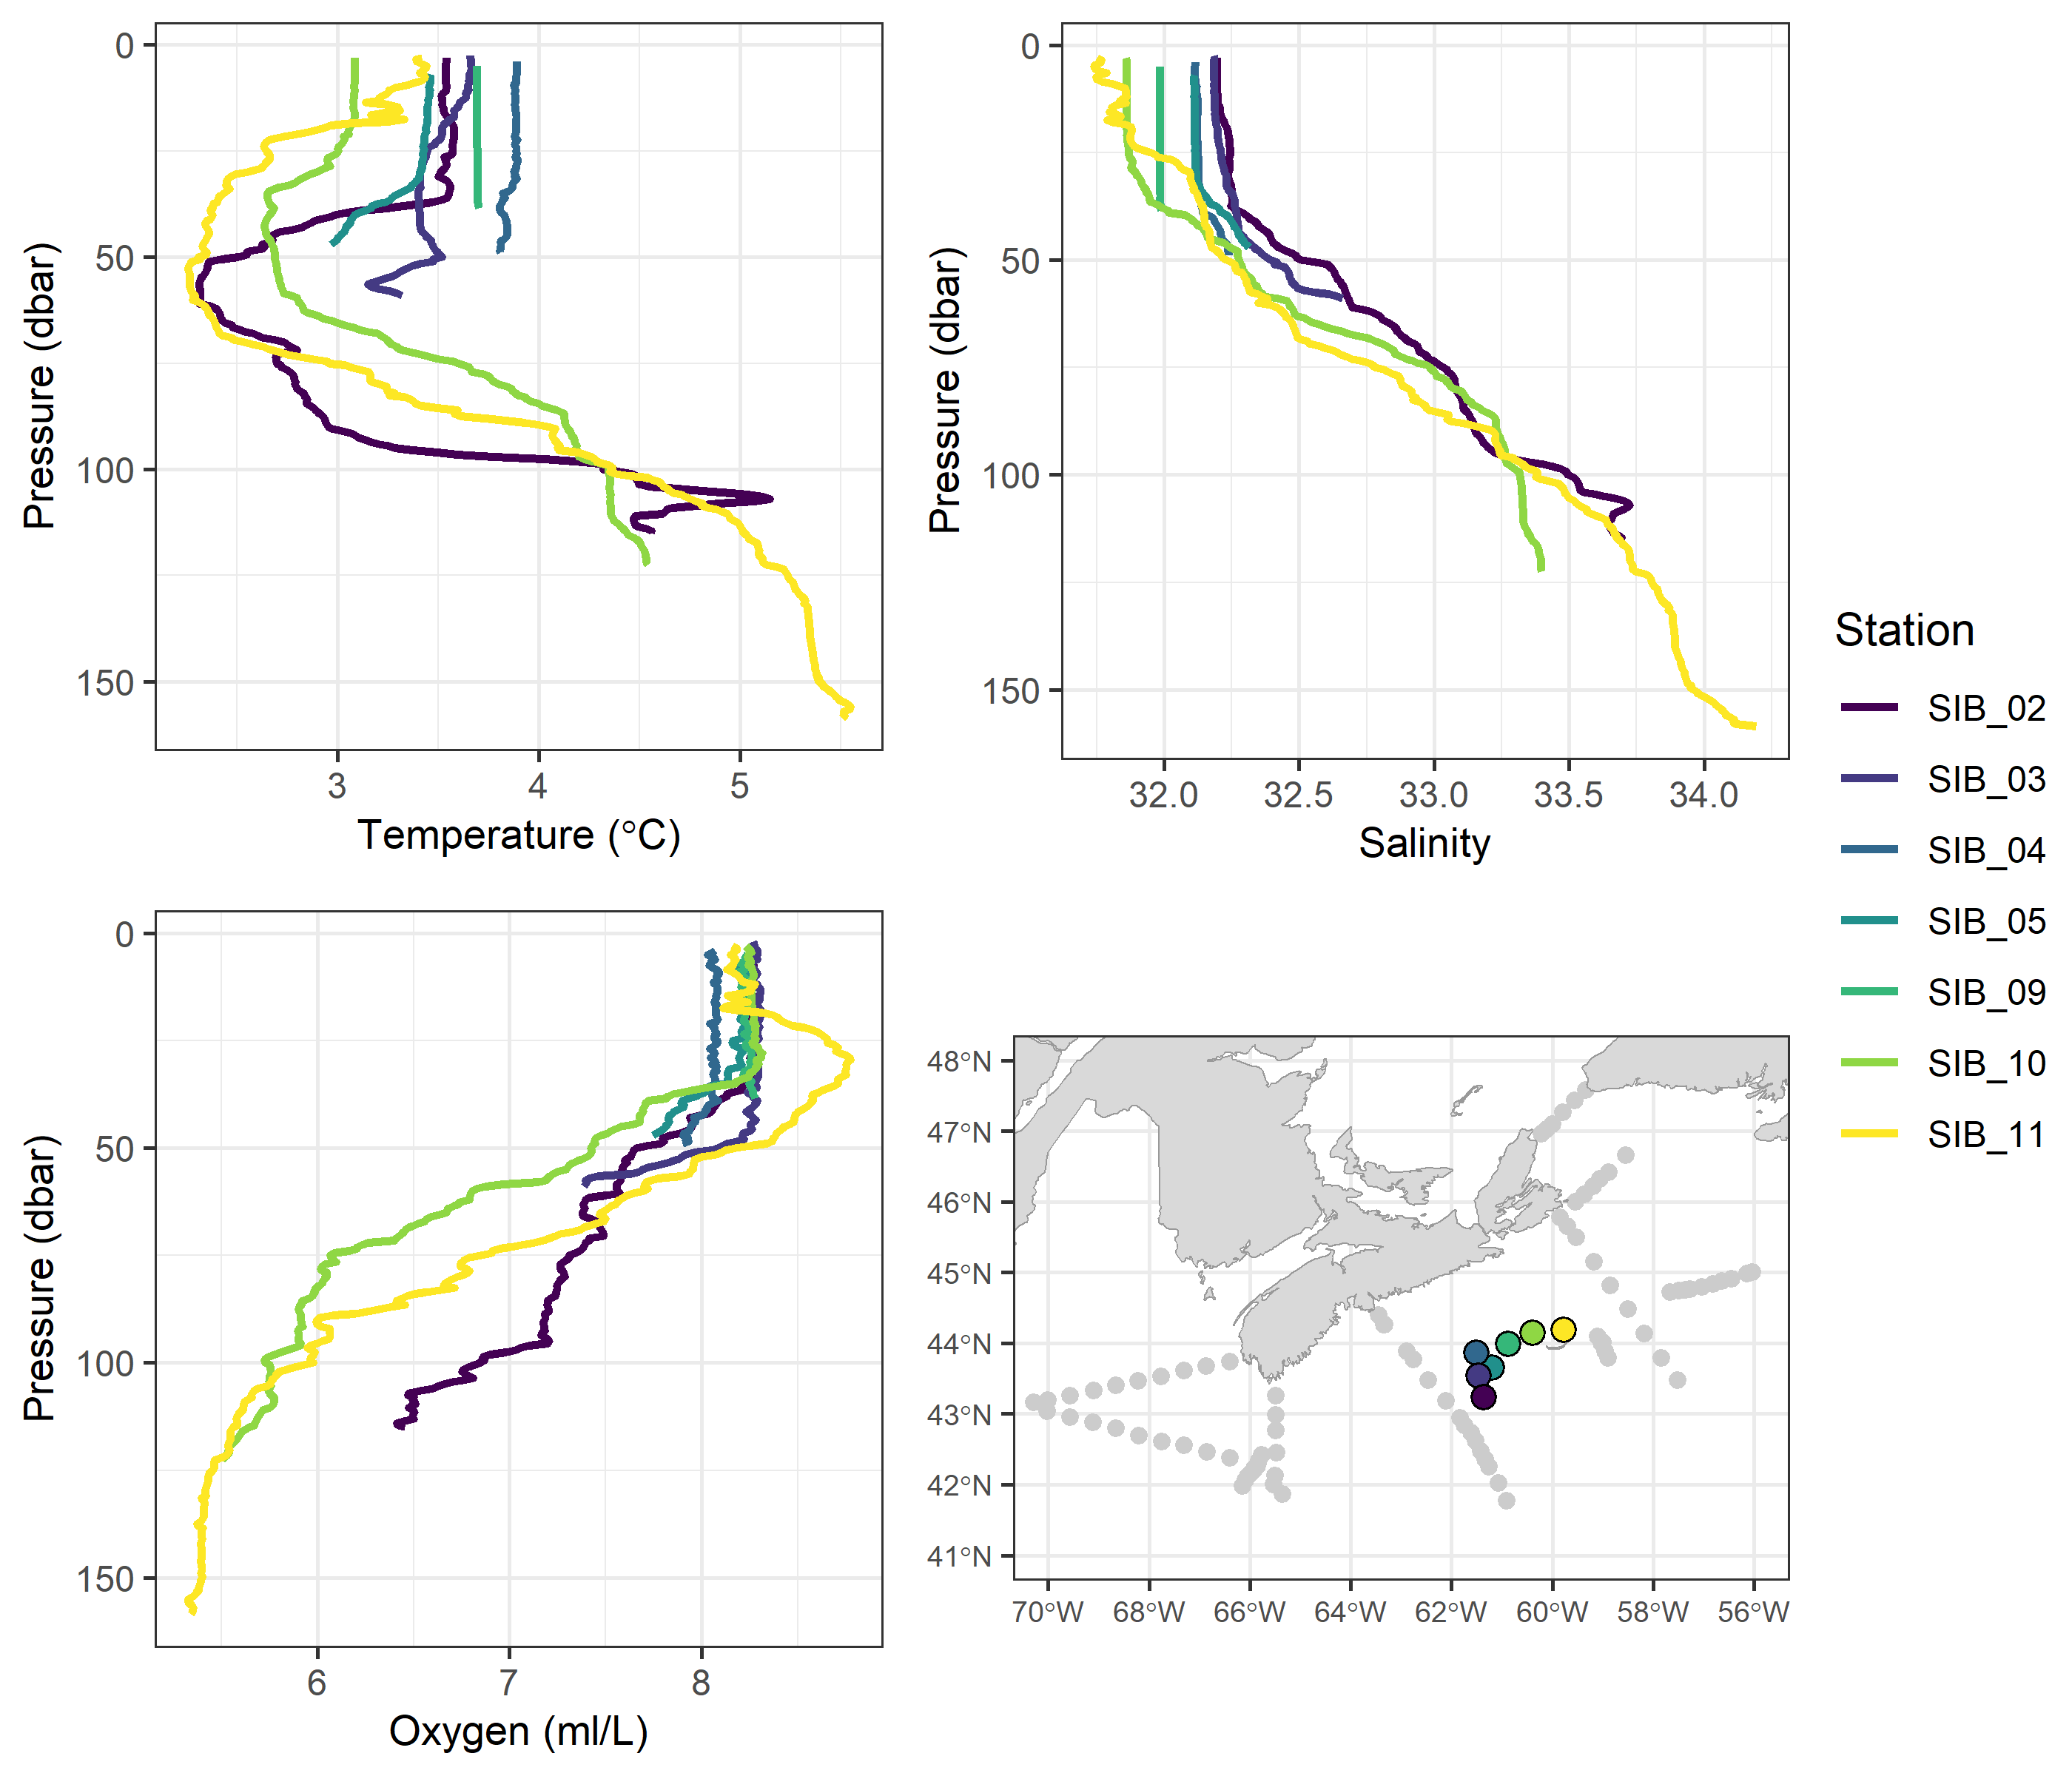
\includegraphics[width=1\linewidth]{figs/EN728_Sable Island Bank_VerticalProfiles}}{Figure} 

}

\caption{Vertical profiles of temperature (top left), salinity (top right), and dissolved oxygen (bottom left) from stations sampled on Sable Island Bank (SIB; bottom right) during the 2025 spring AZMP mission (EN728).}\label{fig:figureA11}
\end{figure}
\clearpage

\end{appendices}
\end{document}
